\documentclass{article}

%%%%%%%%%%%%%%%%%%%%%%%%%%%%%%%%%%%%%%%%%%%%%%%%%%%%%%%%%%%%%%%%%%%%%%%%%%%%%%%%
%% package setup
%%%%%%%%%%%%%%%%%%%%%%%%%%%%%%%%%%%%%%%%%%%%%%%%%%%%%%%%%%%%%%%%%%%%%%%%%%%%%%%%

%\usepackage{enumerate}
\usepackage[shortlabels]{enumitem}
\usepackage{amsfonts, amsmath, amsthm, amssymb, float, mathtools, bbm, etoolbox, xcolor, enumitem}
\usepackage[hyperfootnotes=false, linktocpage=true]{hyperref}
%\usepackage{soul, matlab-prettifier, multirow, varwidth, array, bm, amssymb}
%\usepackage[all]{xy}
\usepackage[margin=1.3in]{geometry}
%\usepackage{graphicx}
\usepackage{extarrows, multirow}
\usepackage{tikz}
\usepackage{tikz-cd}
%\usepackage{bbold}
\usepackage[OT2,T1]{fontenc}
\usepackage{calrsfs}
\usepackage{dsfont}
\usepackage[title]{appendix}
\usepackage{wrapfig}
\usepackage{subcaption}

%%%%%%%%%%%%%%%%%%%%%%%%%%%%%%%%%%%%%%%%%%%%%%%%%%%%%%%%%%%%%%%%%%%%%%%%%%%%%%%%
%% operators and symbols
%%%%%%%%%%%%%%%%%%%%%%%%%%%%%%%%%%%%%%%%%%%%%%%%%%%%%%%%%%%%%%%%%%%%%%%%%%%%%%%%

\newcommand{\define}[4]{\expandafter#1\csname#3#4\endcsname{#2{#4}}}


% operators
\forcsvlist{\define{\DeclareMathOperator}{\mathrm}{}}{Ad, Aut, B, BSD, Char, Cl, Det, End, Frob, Gal, GL, hol, Hom, I, II, III, IV, Id, Ind, Irr, Jac, Ker, Mod, N, new, old, ord,  Perm, PGL, Pic, Proj, PSL, R, Rad, Reg, Rep, res, Res, rk, sign, SL, Smo, SO, Span, Spec, Stab, supp, sw, Sym, Ta, tors, Tr, Trace, un, Vect, contr, Sel, rad, Norm}

%trivial and ell
\newcommand{\trivial}{\mathbbm{1}}
%\renewcommand{\ell}{l}

%mathbb letters 
\forcsvlist{\define{\newcommand}{\mathbb}{b}}{1,A,B,C,D,E,F,G,H,I,J,K,L,M,N,O,P,Q,R,S,T,U,V,W,X,Y,Z, c}

%mathcal letters
\forcsvlist{\define{\newcommand}{\mathcal}{c}}{A,B,C,D,E,F,G,H,I,J,K,L,M,N,O,P,Q,R,S,T,U,V,W,X,Y,Z,a,v, c}

%mathfrak letters
\forcsvlist{\define{\newcommand}{\mathfrak}{f}}{A,B,C,D,E,F,G,H,I,J,K,L,M,N,O,P,Q,R,S,T,U,V,W,X,Y,Z,a,m,n,p,q, g, t, c, f, s}

%overline letters
\forcsvlist{\define{\newcommand}{\overline}{ov}}{H,I,J,K,L,M,N,O,P,Q,R,S,T,U,V,W,X,Y,Z,a,b,c,d,e,f,g,h,i,j,k,l,m,n,o,p,q,r,s,t,u,v,w,x,y,z}

% mathbb
\newcommand{\CC}{\mathbb{C}}
\newcommand{\FF}{\mathbb{F}}
\newcommand{\NN}{\mathbb{N}}
\newcommand{\PP}{\mathbb{P}}
\newcommand{\QQ}{\mathbb{Q}}
\newcommand{\RR}{\mathbb{R}}
\newcommand{\ZZ}{\mathbb{Z}}
\newcommand{\GG}{\mathbb{G}}
\newcommand{\adele}{\mathbb{A}}
\newcommand{\pp}{\mathfrak{p}}
\newcommand{\qq}{\mathfrak{q}}
\newcommand{\rr}{\mathfrak{r}}

% mathfra
%\newcommand{\fg}{\mathfrak{g}}
%\newcommand{\fm}{\mathfrak{m}}

\newcommand{\norm}[1]{\left\lVert#1\right\rVert}
\newcommand{\hatv}[1]{\overset{\vee}{\mathstrut#1}}
\newcommand{\legendre}[2]{\ensuremath{\left( \frac{#1}{#2} \right) }}
\newcommand{\repnorm}[1]{\fN_{\bQ(#1) / \bQ}(#1)}
\newcommand{\fieldnorm}[1]{N_{\bQ(#1) / \bQ}(\bQ(#1)^{\times})}
\newcommand{\defeq}{\mathrel{\mathop:}=} 
\newcommand{\C}{\hat{C}}
\newcommand{\QQss}{(\QQ^{\times})^2}
\newcommand{\Dp}{D_{\fP\mid\fp}}
\newcommand{\Cp}{C_{\fP\mid\fp}}
\newcommand{\Tp}{T_{\fP\mid\fp}}
\newcommand{\Dpb}{D_{\fP\mid\bar\fp}}
\newcommand{\Cpb}{C_{\fP\mid\bar\fp}}
\newcommand{\Tpb}{T_{\fP\mid\bar\fp}}


% Structures
\def\set#1{\left\{#1\right\}}
%\def\sets#1#2{\left\{\left.#1\ \right\vert#2\right\}}
\def\rbr#1{\left(#1\right)}
\def\ang#1{\left\langle#1\right\rangle}
\def\n#1{\left\lvert#1\right\rvert}
\def\nn#1{\left\lVert#1\right\rVert}
\def\eq#1{\begin{equation}#1\end{equation}}
\def\ov#1#2{{\substack{#1\\#2}}} % #1 over #2

% Symbols
\def\mto{\mapsto}
\def\emb{\hookrightarrow}
\def\es{\emptyset}
\def\bs{\backslash}
\def\cupp{\smallsmile}
\def\surj{\twoheadrightarrow}

% floor and ceiling
\DeclarePairedDelimiter\ceil{\lceil}{\rceil}
\DeclarePairedDelimiter\floor{\lfloor}{\rfloor}

\DeclareMathOperator{\Ima}{Im}
%\linespread{1.5}

\theoremstyle{plain}
\newtheorem{thm}{Theorem}[section]
\newtheorem{question}[thm]{Question}
\newtheorem{prop}[thm]{Proposition}
\newtheorem{condition}[thm]{Condition}
\newtheorem{lemma}[thm]{Lemma}
\newtheorem{cor}[thm]{Corollary}
\newtheorem{algo}[thm]{Algorithm}
\theoremstyle{definition}
\newtheorem{defn}[thm]{Definition}
\newtheorem{notn}[thm]{Notation}
\newtheorem{rem}[thm]{Remark}
\newtheorem{example}[thm]{Example}
\newtheorem{exercise}[thm]{Exercise}
\newtheorem{examples}[thm]{Examples}
\newtheorem{fact}[thm]{Fact}
\newtheorem{problem}[thm]{Problem}

\newtheorem{conj}[thm]{Conjecture}
\newtheorem*{conj*}{Conjecture}
\newtheorem{notation}[thm]{Notation}
\newtheorem*{thm*}{Theorem}

%Sha:
\usepackage[OT2,T1]{fontenc}
\DeclareSymbolFont{cyrletters}{OT2}{wncyr}{m}{n}
\DeclareMathSymbol{\Sha}{\mathalpha}{cyrletters}{"58}
%end of Sha

%\DeclareSymbolFont{cyrletters}{OT2}{wncyr}{m}{n}
%\DeclareMathSymbol{\Sha}{\mathalpha}{cyrletters}{"58}

%\DeclareMathAlphabet{\pazocal}{OMS}{zplm}{m}{n}

\title{Arithmetic Applications of Artin Twist and BSD}
\author{Edwina Aylward, Albert Lopez Bruch}
%\date{}

\begin{document}
	\maketitle	\thispagestyle{empty}
	%\newpage
	{\abstract{Let $E / \bQ$ be an elliptic curve, $F / \bQ$ a Galois extension. We investigate a new test introduced in \cite{DEW1} that can force $E$ to have positive rank over $F$. This test appears very different to existing parity tests. We show that one cannot use this test to force positive rank when $F / \bQ$ is a cyclic or odd degree extension.}}
	\tableofcontents
	\pagenumbering{arabic}	
	\setcounter{page}{1}
	%\newpage

\section{Introduction}
The Birch--Swinnerton-Dyer conjecture is one the most important and celebrated statements in classical algebraic number theory, and has been driving large amounts of current research in the area. The statement conjecturally provides a bridge between the arithmetic of elliptic curves, or abelian varieties more generally, and the properties of their associated L-functions, a (conjecturally) meromorphic function in the complex plane, and therefore an analytic object in nature. This connection between arithmetic and analytic objects is ubiquitous throughout pure mathematics, and it has remarkable and surprising consequences, many of which are deep and non-trivial. The BSD conjecture for elliptic curves establishes the following connection.

\begin{conj}[BSD Conjecture]
    Let $E$ be an elliptic curve over a number field $F$, and let $L(E/F,s)$ be the associated L-function. Then
    \begin{equation}\label{eqn_BSD1}\tag{BSD1}
        \quad\ord_{s=1}L(E/F,s)=\rk E/F,
    \end{equation}
    and the leading term of the Taylor series at $s=1$ of $L(E/F,s)$ is given by
    \begin{equation}\label{eqn_BSD2}\tag{BSD2}
        \lim_{s\to1}\frac{L(E/F,s)}{(s-1)^r}\cdot\frac{\sqrt{|\Delta_F|}}{\Omega_+(E)^{r_1+r_2}|\Omega_-(E)|^{r_2}}=\frac{\Reg_{E/F}|\Sha_{E/F}|C_{E/F}}{|E(F)_{\tors}|^2},
    \end{equation}
    where $r$ is the order of the zero of $L(E/F,s)$ at $s=1$, $(r_1,r_2)$ is the signature of $F$, $\Omega_{\pm}$ are the periods of $E$, $\Reg_{E/F}$ is the regulator, $\Sha_{E/F}$ is the Tate-Shafarevich group and $C_{E/F}$ is a product of local terms depending on the primes in $F$ of bad reduction over $E$ (see Section \ref{sec_BSD}).
\end{conj}

In this document, we investigate the arithmetic consequences of the factorization of L-functions of elliptic curves over number fields, commonly known as Artin formalism. Dokchitser, Evans and Wiersema in \cite{DEW1} have already studied some of these and, in particular, they constructed a test that predicts positive rank for families of elliptic curves, which is only dependent on certain local arithmetic data associated to the primes of bad reduction of the elliptic curve. The existence of such tests, which we call `Norm Relations tests', is encoded in the following statement. 

\begin{conj}\cite[Theorem 33]{DEW1}\label{conj_normstest}
    Let $E/\QQ$ be an elliptic curve, $F/\QQ$ a finite Galois extension with Galois group $G$, $\rho$ an Artin representation over $\bQ$ that factors through $G$ and 
    \begin{equation}\label{eqn_localterms}\tag{\textdagger}
        \left(\bigoplus_{\mathfrak{g}\in\Gal(\QQ(\rho)/\QQ)}\rho^{\mathfrak{g}}\right)^{\oplus m}=\bigoplus_i\Ind_{F_i/\QQ}\mathds{1}\ominus\bigoplus_j\Ind_{F'_j/\QQ}\mathds{1}
    \end{equation}
    for some $m\geq 1$ and subfields $F_i,F'_j\subseteq F$. If either $\frac{\prod_i C_{E/F_i}}{\prod_j C_{E/F'_j}}$ is not a norm from some quadratic subfield $\QQ(\sqrt{D})\subseteq\QQ(\rho)$, or if it is not a rational square when $m$ is even, then $E$ has a point of infinite order over $F$.
\end{conj}

In the above conjecture, $\QQ(\rho)$ is the field obtained by attaching $\{\Tr(\rho(\fg)):\fg\in\Gal(K/\QQ)\}$, which is a Galois abelian extension of $\QQ$, and $\rho^{\fg}$ is the representation with character given by $\Tr\circ\rho^{\fg}=(\Tr\circ\rho)^{\fg}$ for $\fg\in\Gal(\QQ(\rho)/\QQ)$, denoted as the twist of $\rho$ by $\fg$.

%% This conjecture holds given stuff

Let us briefly describe an example where Conjecture \ref{conj_normstest} indeed predicts positive rank. We revisit this example in detail in Section \ref{sec_examples}.

\begin{example}[Example \ref{ex-C2C6}]
    Let $F/\QQ$ be a finite Galois extension such that $\Gal(F/\QQ)=C_2\times C_6$, which has the following subfield diagram.
    \begin{figure}[H]
        \centering
        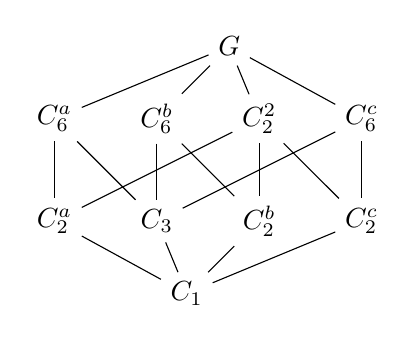
\begin{tikzpicture}[node distance=1.3cm]
            \node(G)[midway]{$G$};
            \node(C6b)[below left of =G]{$C_6^{b}$}; \node(C6a)[left of=C6b]{$C_6^{a}$};  
            \node(C22)[right of=C6b]{$C_2^{2}$};    \node(C6c)[right of=C22]{$C_6^{c}$};
            \node(C2a)[below of=C6a]{$C_2^{a}$};    \node(C3)[below of=C6b]{$C_3$};
            \node(C2b)[below of=C22]{$C_2^{b}$};    \node(C2c)[below of=C6c]{$C_2^{c}$};
            \node(C1)[below left of=C2b]{$C_1$};
            \draw(G)--(C6a);    \draw(G)--(C6b);    \draw(G)--(C6c);    \draw(G)--(C22);
            \draw(C6a)--(C2a);  \draw(C6a)--(C3);
            \draw(C6b)--(C2b);  \draw(C6b)--(C3);
            \draw(C6c)--(C2c);  \draw(C6c)--(C3);
            \draw(C22)--(C2a);  \draw(C22)--(C2b);  \draw(C22)--(C2c);
            \draw(C2a)--(C1);   \draw(C2b)--(C1);   \draw(C2c)--(C1);   \draw(C3)--(C1); 
        \end{tikzpicture}
    \end{figure}
    Let $E/\QQ$ be an elliptic curve such that it has multiplicative reduction at a prime $p$ with decomposition group $G$ and inertia group $C_6^b$ and such that every other prime of bad reduction is unramified in $F/\QQ$. If $\rho$ is an order $6$ character of $G$ with kernel $C_2^a$, then $\QQ(\rho)=\QQ(\zeta_6)=\QQ(\sqrt{-3})$. Following Conjecture \ref{conj_normstest}, we aim to compute 
    \begin{equation*}\label{eqn-rel2}
        \left(\frac{C_{E / F^{C_2^a}} C_{E / \bQ} }{C_{E / F^{C_6^a}} C_{E / F^{C_2^2}}}\right) \cdot \left( \frac{C_{E / F^{C_3}} C_{E / \bQ}^2}{C_{E / F^{C_6^a}}C_{E / F^{C_6^b}}  C_{E / F^{C_6^c}} } \right).
    \end{equation*}
    We remark that the underlying fields do satisfy the condition \eqref{eqn_localterms} from Conjecture \ref{conj_normstest}. This evaluates to $2\cdot\square$, and since $2$ is not a norm of an element from $\QQ(\sqrt{-3})$, Conjecture \ref{conj_normstest} forces $\rk E/F>0$. 
\end{example}

This test of predicting positive rank for families of elliptic curves should be reminiscent of using root number computations to predict positive rank based on local data. One takes the product of local roots numbers to obtain a global root number $w(E/K)\in{\pm1}$, and this arises in the (conjectural) functional equation of $L(E/K,s)$ (see Conjecture \ref{conj_hasseweil}). Hence, it describes the parity of the vanishing of the L-function at $s=1$. Assuming BSD, one expects the following to hold.

\begin{conj}[Parity Conjecture]\label{conj_parity}
    Let $E$ be an elliptic curve over a number field $K$. Then
    $(-1)^{\rk E / K} = w(E / K).$
\end{conj}

Using the Parity Conjecture to test for rank growth is known as a `parity test'. The Parity Conjecture has been extensively studied in the literature, see for example \cite{Tim} It is known to hold in certain conditions under the assumption of finiteness of $\Sha_{E/F}$. One can observe that the rank growth in the above example can also be explained by the Parity Conjecture, and we expect this phenomenon to happen in general. 

\begin{conj}\label{conj_normroot}
    Consider an elliptic curve $E / \bQ$, $F / \bQ$ a finite Galois extension, and relation 
    $$\left(\bigoplus_{\mathfrak{g}\in\Gal(\QQ(\rho)/\QQ)}\rho^{\mathfrak{g}}\right)^{\oplus m}=\bigoplus_i\Ind_{F_i/\QQ}\mathds{1}\ominus\bigoplus_j\Ind_{F'_j/\QQ}\mathds{1}$$
    as in \eqref{eqn_localterms}. If the product $\frac{\prod_i C_{E/F_i}}{\prod_j C_{E/F'_j}}$ is not a norm from some quadratic subfield $\QQ(\sqrt{D})\subseteq\QQ(\rho)$, or if it is not a rational square when $m$ is even, then there exists a subfield $K\subseteq F$ such that $w(E/K)w(E/\QQ)=-1$. 
\end{conj}

In Section \ref{sec-norm-rels-test} we describe a refined version of this conjecture, where it is phrased in terms of Artin twists of root numbers.

Parity tests cannot predict rank growth of elliptic curves in odd degree extensions. This is a direct consequence of the fact that odd degree groups have no non-trivial self dual representations (see Lemma \ref{lem_oddroot}). Accordingly, Norm Relations tests cannot make such a prediction either.

\begin{thm}[Theorem \ref{odd-exts}]\label{thm_odd-cons}
    Let $E / \bQ$ be an elliptic curve and let $F / \bQ$ be a Galois extension of odd order with Galois group $G$. Assume that $E$ has semistable reduction at $2$ and $3$ and take any representation $\rho$ of $G$. Suppose $m\geq 1$ and $F_i,F_j'\subseteq F$ satisfy 
    \begin{equation*}%\label{odd-exp} 
        \left(\bigoplus_{\mathfrak{g}\in\Gal(\QQ(\rho)/\QQ)}\rho^{\mathfrak{g}}\right)^{\oplus m }=\bigoplus_i\Ind_{F_i/\QQ}\mathds{1}\ominus\bigoplus_j\Ind_{F'_j/\QQ}\mathds{1}.
    \end{equation*}
    Then, for any $\QQ(\sqrt{D})\subseteq\QQ(\rho)$, we have that
    \[ \frac{\prod_i C_{E/F_i}}{\prod_j C_{E/F_j'}}  \in 
       \begin{cases}
           N_{\bQ(\sqrt{D}) / \bQ}(\bQ(\sqrt{D})^{\times}) & m \ \text{odd}, \\
           (\bQ^{\times})^2 & m \ \text{even}.
       \end{cases} 
    \] 
       %In other words, one cannot use Theorem \ref{thm_positive_rank} to conclude that $E / F$ must have positive rank. 
\end{thm}

%and this is indeed the case. In Sections \ref{sec_cyclic} and \ref{sec_odd} we describe two general settings in which Norm Relation test can never predict rank growth. One such setting is odd degree extensions.

The other setting in which Norm Relation tests cannot predict rank growth is when $F/\QQ$ is a Galois cyclic extension. When $G=\Gal(F/\QQ)$ is even and cyclic, parity tests can predict rank growth through the sign representation, which is a self-dual representation. However, for Norm Relation tests, the following holds.

\begin{thm}[Theorem \ref{thm_consistent_cyclic}]\label{thm_cyclic-cons}
    Let $d\geq2$ be a positive integer and let $F/K$ be a Galois extension of number fields such that $\Gal(F/K)=C_d$. Take any representation $\rho$ of $C_d$ and any semistable elliptic curve $E/\QQ$ at $2$ and $3$. 
    
    Let $F_i,F_j'$ be the intermediate fields of $F/K$ (which exist and are unique up to permutation) such that 
    \begin{equation*}%\label{odd-exp} 
        \bigoplus_{\mathfrak{g}\in\Gal(\QQ(\rho)/\QQ)}\rho^{\mathfrak{g}}=\bigoplus_i\Ind_{F_i/K}\mathds{1}\ominus\bigoplus_j\Ind_{F'_j/K}\mathds{1}
    \end{equation*}
    Then, for any $\QQ(\sqrt{D})\subseteq\QQ(\rho)$, we have that
    $$\frac{\prod_i C_{E/F_i}}{\prod_j C_{E/F_j'}}\in N_{\QQ(\sqrt{D})/\QQ}(\QQ(\sqrt{D})^{\times}).$$
\end{thm}

The strategy to prove these results is to break down the product 
$$\frac{\prod_i C_{E/F_i}}{\prod_j C_{E/F_j'}}=\prod_{\pp}\left(\frac{\prod_i \Cp(E/F_i)}{\prod_j \Cp(E/F_j')}\right)$$
into the local contributions of each prime $\pp$ in the base field (see Notation \ref{not_contr}). Each one of these local factors depends on the decomposition group $D_\pp\leq G$ and inertia group $I_\pp\triangleleft D_\pp$. Consequently, the following corollary also holds.

\begin{cor}[Corollary \ref{cor-odd-cyclic-decomp}]%\label{cor-odd-cyclic-decomp}
    Let $E / \bQ$ be an elliptic curve, $F / \bQ$ a Galois extension with Galois group $G$. Assume that $E$ has good or multiplicative reduction at $2$ and $3$. 
    
    Let $\rho$ be a representation of $G$, and let $m\geq 1$ and $F_i,F_j'\subseteq F$ be as in \eqref{eqn_localterms}. Let $p$ be a rational prime and suppose that $D_p\leq G$ is either cyclic or a group of odd order. Then, for any $\QQ(\sqrt{D})\subseteq\QQ(\rho)$, one has
    \[
        \frac{\prod_i C_{\fP\mid p}(E/F_i)}{\prod_j C_{\fP\mid p}(E/F_j')}\in
        \begin{cases}
            N_{\QQ(\sqrt{D})/\QQ}(\QQ(\sqrt{D})^{\times}) & \text{ $m$ odd,}\\ \QQss & \text{ $m$ even.}
        \end{cases}
    \] 
\end{cor}

Therefore, when trying to use Norm Relations tests to force positive rank, interesting cases can only occur when $E/\QQ$ has bad reduction at primes that ramify in $F/\QQ$ and such that $D_p$ is non-cyclic and has even order.

\subsection*{Layout of the Report}
The purpose of this project is two-fold: firstly, it aims to serve as an introduction to the topics related to the Birch--Swinnerton-Dyer conjecture and, secondly, it studies the arithmetic consequences of Conjecture \ref{conj_normstest} for elliptic curves.

Sections \ref{sec_EC} to \ref{sec_BSD} serve the first purpose. In Section \ref{sec_EC}, we give a brief and rather informal discussion on the theory of elliptic curves, where we dedicate most of our attention in describing their local behaviour. 
%Of course, we assume familiarity with the topic, but we give appropriate references for those results that are generally less known or harder to find in the literature. 
In Section \ref{sec_Lside}, we introduce the notion of an Artin representation and $\ell$-adic representation, and we also give a detailed description on the construction of the L-functions $L(E/F,s)$ associated to an elliptic curve over a number field $F$ and of its twist by an Artin representation $\rho$. Finally, in Section \ref{sec_BSD} we discuss the BSD conjecture in more detail and we explain the arithmetic terms appearing in the statement of the conjecture. We also discuss an important conjectural analogue of BSD for Artin twists which naturally leads to the statement of Conjecture \ref{conj_4}, which motivates the latter half of the discussion.

The remaining sections serve the second purpose of studying the arithmetic of elliptic curves through Conjecture \ref{conj_4}. In Section \ref{sec_pos_rank} we describe how to derive Conjecture \ref{conj_normstest} from the statement of Conjecture \ref{conj_4}, and we provide detailed examples on how Norm Relations test predict positive rank. The statement and proofs of Theorems \ref{thm_odd-cons} and \ref{thm_cyclic-cons} are more naturally phrased in representation theoretic terms. Therefore, in Section \ref{sec_norm}, we introduce the necessary notation and results required for the later sections. 

The last three sections of the report are devoted to proving Theorems \ref{thm_odd-cons} and \ref{thm_cyclic-cons}. In Section \ref{sec_preliminary}, we prove some preliminary results that describe the local behaviour of some families of elliptic curves. Sections \ref{sec_cyclic} and \ref{sec_odd} contain the main proofs of the report on the cyclic and odd cases, respectively. At the end of the report, the reader can find the Appendix with some global class field theory that are used throughout the latter sections.

\subsection*{Acknowledgements}

We would like to thank our supervisor Vladimir Dokchitser for his generosity with his time, his many helpful suggestions, and for introducing us to this interesting topic.


\newpage
\section{Elliptic Curves}\label{sec_EC}

Having discussed the relevant aspects of representation theory that we will require, we now introduce elliptic curves, our main object to study. Our discussion will be rather informal and brief, and will avoid most proofs. We will spend some time discussing the reduction type of elliptic curves and how this can change over finite extensions. Nevertheless, we assume good familiarity with elliptic curves. There is great material available for elliptic curves, and \cite{S1} gives a complete discussion.

An elliptic curve $E$ over a field $K$ is a genus one smooth projective curve with a specified $K$-rational point. Any such curve can be written as the locus on $\PP^2$ of a \textbf{Weierstrass equation}
\begin{equation}\label{eqn_gen_elliptic}
    E: y^2+a_1xy+a_3y=x^3+a_2x^2+a_4x+a_6,\quad a_2,a_4,a_6\in K,
\end{equation}
together with the specified $K$-rational point $[0:1:0]$ at infinity.

When $\Char(K)\neq2$, which will always be the case, we can further simplify the equation to
\begin{equation}\label{eqn_elliptic}
    E: y^2=f(x)=x^3+a_2x^2+a_4x+a_6,\quad a_2,a_4,a_6\in K,
\end{equation}
so unless stated otherwise we will assume that $E$ has an equation of this form. We remark that if $\Char(K)=2$, then \eqref{eqn_elliptic} always defines a singular curve. Associated to this equation there are constants 
$$c_4=16(a_2^2-3a_4) \quad\text{and}\quad \Delta=16(a_2^2a_4^2-4a_2^3a_6-4a_4^3-27a_6^2+18a_2a_4a_6)$$
and differential 
\begin{equation}\label{eqn_differential}
    w=\frac{dx}{2y}=\frac{dy}{3x^2+2a_2x+a_4}.
\end{equation}
One can also define these constants for the general Wieirstrass equation \eqref{eqn_gen_elliptic}, but we omit the description. A complete description is given in \cite[\S III.1]{S1}

The curve defined by \eqref{eqn_elliptic} is singular if and only if the polynomial $f(x)$ has repeated roots over $\bar{K}$. If it has a double and a simple root, then we say it has a node; if it has a triple root, then it has a cusp. The following proposition characterizes this behaviour in terms of $c_4$ and $\Delta$.

\begin{prop}\label{prop_nodecusp}
    The curve given by a Weierstrass equation satisfies:
    \begin{enumerate}
        \item It is nonsingular if and only if $\Delta\neq0$.
        \item It has a node if and only if $\Delta=0$ and $c_4 \neq 0$.
        \item It has a cusp if and only if $\Delta= c_4 = 0$. 
    \end{enumerate}
\end{prop}
\begin{proof}
    \cite[\S III Proposition 1.4]{S1}.
\end{proof}

When $\Delta\neq0$, the equation defines an elliptic curve. A fundamental property is that the set of $K$-rational points of an elliptic curve forms an abelian group, denoted by $(E(K),\oplus)$ (\cite[\S III.2]{S1}). When $K$ is a number field, the Mordell-Weil theorem shows that this group is also finitely generated, and therefore 
$$E(K)=E(K)_{\tors}\times\ZZ^r,$$
where $E(K)_{\tors}$ is a finite abelian group and $r$ is denoted the rank of $E$.

\subsection{Elliptic Curves over Local Fields and Reduction Types}

Now assume that $K$ is a local field of characteristic $0$ with a discrete valuation $\nu$, ring of integers $R$ and residue field $\kappa$. We denote by $a\mapsto \tilde{a}$ for the natural quotient map $K\to\kappa$. We say that \eqref{eqn_elliptic} is a \textbf{minimal Weierstrass equation} if $a_2,a_4,a_6\in R$ and $\nu(\Delta)$ is minimal among all such equations. When this is the case, we have a well-defined associated curve $\tilde{E}$ over $\kappa$ defined by the equation $y^2=x^3+\tilde{a_2}x^2+\tilde{a_4}x+\tilde{a_6}$ and the associated \textbf{reduction map}
\begin{equation}\label{eqn_reduction}
    \widetilde{(\cdot)}:E(K)\longrightarrow \tilde{E}(\kappa),
\end{equation}

obtained by reducing the coordinates of a point $P\in E(K)$ modulo $\kappa$. One needs to have some care defining the reduction map. For a detailed construction, see \cite[\S1 VII.2]{S1}. We remark that $\tilde{E}$ may be a singular curve, and the \textbf{reduction type} of $E$ over $K$ describes the behaviour of $\tilde{E}$ as a curve over $\kappa$.

\begin{defn}
    Let $E/K$ and $\tilde{E}/\kappa$ be as above. Then we say that 
    \begin{enumerate}[label={(\alph*)}]
        \item $E/K$ has good (or stable) reduction if $\tilde{E}$ is non-singular.
        \item $E/K$ has multiplicative (or semistable) reduction if $\tilde{E}$ has a node.
        \item $E/K$ has additive (or unstable) reduction if $\tilde{E}$ has a cusp.
    \end{enumerate}
    In cases (b) and (c) we say that $E/K$ has bad reduction. Moreover, if $E/K$ has multiplicative reduction, we say that the reduction is split if the slopes of the tangent lines at the node are in $K$, and non-split otherwise.
\end{defn}

By Proposition \ref*{prop_nodecusp} we immediately see that $E/K$ has good reduction if $\nu(\Delta)=0$ and bad otherwise. In that case, $E/K$ has multiplicative reduction if $\nu(c_4)=0$ and additive otherwise.

An important question which will be of interest for us is to understand how the reduction type of an elliptic curve $E$ changes over a finite field extension $F/K$. The following proposition gathers this information.

\begin{prop}[Semistable reduction Theorem]
    Let $E$ be an elliptic curve over a local field $K$ of characteristic $0$. 
    \begin{enumerate}[label={(\roman*)}]
        \item Let $F/K$ be an unramified extension. Then the reduction type of $E$ over $K$ (good multiplicative or additive) is the same as the reduction type of $E$ over $F$.
        \item Let $F/K$ be a finite extension. If $E$ has good or multiplicative reduction over $K$, then it has the same reduction type over $F$. This also applies specfically to split multiplicative reduction.
        \item If $E$ has non-split multiplicative reduction over $K$ and $F/K$ is a finite extension with even residual degree, then $E$ has split multiplicative reduction over $F$. 
        \item There exists a finite extension $F/K$ such that $E$ has either good or spit multiplicative over $F$.
    \end{enumerate}
\end{prop}
\begin{proof}
    \cite[\S VII Proposition 5.4]{S1} 
\end{proof}

Given an unstable elliptic curve $E$ over $K$, we say that it has potentially good (resp. multiplicative) reduction if it has good (resp. multiplicative) reduction over a finite field extension of $K$.

\subsection{Tamagawa Numbers} \label{subs_tamagawa}

Recall from the previous section that if $E/K$ has bad reduction, then $\tilde{E}$ is not a smooth curve and therefore its $\kappa$-rational points may not form a group. However, the set $\tilde{E}_{ns}(\kappa)$ of non-singular points of $\tilde{E}(\kappa)$ does indeed form a group. The reduction map \eqref{eqn_reduction} is in general not surjective, but it does surject onto $\tilde{E}_{ns}(\kappa)$. It is natural therefore to define $E_0(K)=\{P\in E(K):\widetilde{P}\in\tilde{E}_{ns}(\kappa)\}$, which is also a subgroup of $E(K)$. Importantly, the resulting reduction map 
$$\widetilde{(\cdot)}:E_0(K)\longrightarrow \tilde{E}_{ns}(\kappa)$$
is a surjective homomorphism of abelian groups.
\begin{defn}
    The \textbf{Tamagawa number} of $E/K$ is defined as
    \begin{equation}
        c(E/K):=|E(K)/E_0(K)|.
    \end{equation}
\end{defn}
In later sections we will be concerned in computing Tamagawa numbers. Note that if $E/K$ has good reduction, then $E_0(K)=E(K)$ and therefore $c(E/K)=1$. However, when $E/K$ has bad reduction, this is a hard question to answer in general. Fortunately, this question can always be resolved using Tate's Algorithm (see \cite[\S IV.9]{S2}), and for semistable reduction, Tamagawa numbers have a simple explicit description.

\begin{prop}
    Let $E/K$ have multiplicative reduction, and let $n=\nu(\Delta)$ be the valuation of the minimal discriminant. Then
    \begin{align*}
        c(E/K)=
        \begin{cases}
            n \quad\text{if $E/K$ has split reduction,}\\
            1 \quad\text{if $n$ is odd and $E/K$ is non-split,}\\
            2 \quad\text{if $n$ is even and $E/K$ is non-split}.
        \end{cases}    
    \end{align*}
\end{prop}

The unstable case is harder, but there exists an explicit description for elliptic curves with equation $y^2=x^3+Ax+B$ and residual characteristic is at least $5$. 

\begin{lemma}\label{tamagawa-num}
    Let $F /K / \bQ_p$ be finite extensions and $p \geq 5$. Let 
    $$E:  y^2 = x^3 + Ax + B$$
    be an elliptic curve over $K$ with additive reduction. Let $n=v_K(\Delta)$ be the valuation of the minimal discriminant, and $e$ the ramification index of $K'/K$.

    If $E$ has potentially good reduction, then 
        \[
        \begin{array}{l l l l}
            \gcd(ne, 12) = 2 & \implies & c(E / K') = 1, & \quad (II, II^*) \\
            \gcd(ne, 12) = 3 & \implies & c(E / K') = 2, & \quad (III, III^*) \\
            \gcd(ne, 12) = 4 & \implies & c(E / K') = \begin{cases} 1, & \sqrt{B} \notin K'
                                \\ 3, & \sqrt{B} \in K' \end{cases}, & \quad (IV, IV^*) \\
            \gcd(ne, 12) = 6 & \implies & c(E / K') = \begin{cases} 2, & \sqrt{\Delta} \notin K'
                \\ 1 \ \text{or} \ 4, & \sqrt{\Delta} \in K' \end{cases}, & \quad (I_0^*) \\
            \gcd(ne, 12) = 12 & \implies & c(E / K') = 1. & \quad (I_0)
        \end{array}
        \]
    Moreover, the extensions $K'(\sqrt{B}) / K'$ and $K'(\sqrt{\Delta}) / K'$ are unramified.

    If $E$ has potentially multiplicative reduction of type $I_n^*$ over $K$, and $e$ is odd, then it has Kodaira type $I_{en}^*$ over $K'$. Moreover, 
    \[
        \begin{array}{l l l l}
        2 \nmid n & \implies & c(E / K') = \begin{cases} 2, & \sqrt{B} \not\in K', \\ 4, & \sqrt{B} \in K'. \end{cases} & \quad (I_{ne^*}) \\
        2 \mid n & \implies & c(E / K') = \begin{cases} 2 & \sqrt{\Delta} \not\in K', \\ 4 & \sqrt{\Delta} \in K' \end{cases} & \quad ({I_{ne}^*})   
        \end{array} 
    \]
\end{lemma}

\begin{proof}
    \cite[Lemma 3.22]{reg-const}
\end{proof}

\subsection{Elliptic Curves over Global Fields}

The topics we have discussed so far, such as the reduction type of an elliptic curve and the Tamagawa number, are intrinsically local objects. We now briefly discuss how we can associate these objects to global fields. For simplicity, assume that $E$ is an elliptic curve over a number field $K$, let $\pp$ be a finite place of $K$ and denote $K_\pp$ by the completion of $K$ at $\pp$ with residue field $\kappa_\pp$. Clearly, we have that $E(K)\subseteq E(K_\pp)$ and therefore we can apply the previous description to the curve $E/K_\pp$.

In particular, the reduction type of $E/K$ at $\pp$ is the reduction type of $E/K_\pp$ and the Tamagawa number of $E/K$ at $\pp$ is defined as 
$$c_\pp(E/K):=c(E/K_\pp),$$
and we also define 
$$c(E/K):=\prod_\pp c_\pp(E/K).$$
Finally, we say that a Weierstrass equation \eqref{eqn_gen_elliptic} is a \textbf{global minimal equation} if it is a minimal equation for all finite places $\pp$ of $K$. Even though such an equation does not always exists for any $K$, it does hold for $\QQ$.

\begin{prop}\label{prop_globmin}
    Let $E/\QQ$ be an elliptic curve. Then $E$ has a global minimal Weierstrass equation.
\end{prop}

Throughout the document, we will work with elliptic curves over $\QQ$, so unless stated otherwise we will assume the defining equation is global minimal.

\newpage
\section{Representations, L-functions and Artin Twists}\label{sec_Lside}
The Birch--Swinnerton-Dyer conjecture classically provides a connection between the arithmetic of elliptic curves and their $L$-functions. In this preliminary section, we explore the classical definition of $L$-functions attached to an elliptic curve and their twists, and we explore some of the relevant properties that we will use later on. To do so, we first need to explore the notion of an Artin representation and of an $\ell$-adic representation. The results in this section are self-contained, and the discussion is inspired by a course on elliptic curves by Vladimir Dokchitser.

Throughout this section we fix a field $K$, which will either be a number field or a non-Archimedean local field of characteristic $0$. For convenience, whenever we say local field from now on we refer to a non-Archimedean field of characteristic $0$. We always specify what $K$ is in each context. We also fix an algebraic closure $\bar{K}$ of $K$ and we denote by $G_K$ the absolute galois group $\Gal(\bar{K}/K)$ of $K$. We recall that $G_K$ is a profinite group
$$G_K=\varprojlim_{F}\Gal(F/K),$$
where $F$ ranges over the finite Galois extensions of $K$ and therefore has a natural topology where a basis of open sets is given by $\Gal(\bar{K}/F)$ where $F$ is a finite extension of $K$.

\subsection{Artin Representations and  \texorpdfstring{$\ell$}{TEXT}-adic Representations} \label{subsection_reps}

We begin by recalling the notion of an Artin representation.

\begin{defn}
    Let $K$ be a number field or a local field. An \textbf{Artin representation} $\rho$ over $K$ is a complex finite-dimensional vector space $V$ together with a homomorphism $\rho:G_K\to\GL(V)=\GL_n(\CC)$ such that there is some finite Galois extension $F/K$ with $\Gal(\bar{K}/F)\subseteq\ker\rho$. In other words, $\rho$ factors through $\Gal(F/K)$ for some finite extension $F$ of $K$.
\end{defn}

Hence, an Artin representation can be equivalently viewed as a finite dimensional representation of $\Gal(F/K)$ where $F$ is some finite Galois extension of $K$. Throughout the document, we will use both notions and refer to either of them as Artin representations. Which notion we refer to is always clear from context.

\begin{rem}
    The condition above that $\Gal(\bar{K}/F)\subseteq\ker\rho$ is equivalent to $\ker\rho$ being open in $G_K$. This condition is clearly equivalent to $\rho$ being continuous with respect the discrete topology on $\GL_n(\CC)$. Interestingly, the profinite topology of $G_K$ has an surprising consequence: this condition is also equivalent to continuity with respect to the usual complex topology on $\GL_n(\CC)$. 
    %Necessity is clear, and the proof of sufficiency relies on the fact that under the complex topology, `small' neighbourhoods of the identity in $\GL(V)=\GL_n(\CC)$ do not contain any non-trivial subgroups. Hence, if $\phi:G_K\to\GL(V)$ is continuous with respect to the complex topology and $U$ is such a neighbourhood in $\GL(V)$, then $\phi^{-1}(U)\subseteq\ker\phi$ and $\phi^{-1}(U)$ is open, showing that $\ker\phi$ is open too. 
    Hence, Artin representations are simply continuous group homomorphisms $\rho:G_k\to\GL_n(\CC)$.
\end{rem}

Next, we define the notion of an $\ell$-adic representation, which will be needed to define the $L$-function of an elliptic curve. This is the local analogue of an Artin representation.

\begin{defn}
    Let $K$ be a number field or a local field. A \textbf{continuous $\ell$-adic representation} $\rho$ over $K$ is a continuous homomorphism $\rho:G_K\to\GL_n(F)$ where $F$ is a finite extension of $\QQ_\ell$ and $\GL_n(F)$ is equipped with the $\ell$-adic topology.
\end{defn}

\begin{rem} \label{rem_cont_ladic}
    The topologies on $\GL_n(\CC)$ and $\GL_n(\QQ_\ell)$ are very different, and in particular and $\ell$-adic representation may not have an open kernel. Instead, continuity is equivalent to the following condition: for every $m\geq1$, there is some finite field extension $F_m$ of $K$ such that for all $g\in\Gal(\bar{K}/F_m)$, $\rho(g)\equiv \mathrm{Id}_n\pmod{\ell^m}$.
\end{rem}

Given an Artin representation $\rho$, one can view it as homomorphism $\rho:G_K\to\GL_n(\bar{\QQ})$ and since it factors through a finite quotient, we can realise it as $\rho:G_K\to\GL_n(F)$ for some number field $F$. Hence, if $\ell$ is any rational prime and $\mathfrak{l}$ is a prime in $F$ above $\ell$, then one can realise $\rho$ as an $\ell$-adic representation $$\rho:G_K\longrightarrow\GL_n(F_\mathfrak{l}),$$
which is continuous since $\rho$ factors through a finite quotient. Furthermore, Artin and $\ell$-adic representations over $K$ have more structure; namely, one can take \textbf{direct sums} and \textbf{tensor products} in the natural way.

%We describe the construction for Artin representations, since the $\ell$-adic case is completely analogous. Suppose we have two Artin representations $\rho_1,\rho_2$ over $K$, and by the discussion on the preceding paragraph we can realise them as maps $\rho_i:G_K\to\GL_{n_i}(L_i),\ i=1,2$ where $L_1$ and $L_2$ are number fields. If we let $L=L_1L_2$, then the natural maps $\rho_1\oplus\rho_2:G_K\to\GL_{n_1+n_2}(L)$ and $\rho_1\otimes\rho_2:G_K\to\GL_{n_1n_2}(L)$ are both Artin representations. One can also show that this construction is also well-defined up to equivalence.

Finally, we discuss the notion of an induced Artin representation. Suppose $L$ is a finite field extension of $K$ of degree $d$ and let $\rho:G_L\to\GL(V)$ be an Artin representation. Then $G_L$ is naturally a subgroup of $G_K$ of index $d$, and therefore we can construct $\Ind_{G_L}^{G_K}\rho$ in the usual way. This turns out to be an Artin representation of $K$: if $F$ be a number field so that $\rho$ factors through $\Gal(F/L)$, then $\Ind_{G_L}^{G_K}\rho$ will factor through $\Gal(F/K)$. Furthermore, the corresponding representation over $\Gal(F/K)$ will be equivalent to $\Ind_{\Gal(F/L)}^{\Gal(F/K)}\rho$ where $\rho$ is now viewed as a representation of $\Gal(F/L)$. Hence, the notion of induction is naturally compatible with this process of passing through finite quotients. 

\begin{notn}
We write $\Ind_{L/K}\rho$ for the induced Artin representation, and it will always be clear from context the implicit field $F$.
\end{notn}

%Then one can define the vector space 
%$$X=\{f:G_K\to V:f(\tau\sigma)=\rho(\tau)f(\sigma), \tau\in G_L, \sigma\in G_K\}$$
%and equip it with a $G_K$ action given by $(\sigma\cdot f)(\pi)=f(\pi\sigma)$.
\subsection{Local Polynomials and L-functions}
We now briefly discuss how to attach analytic objects to Artin and $\ell$-adic reperesentations. These objects are usually described for local fields of characteristic $0$ first. Then, one constructs global objects attached to number fields by completing them at their finite places, obtaining the local information and then combinining it appropiately. 

To begin, let $K$ be a local field with $0$ characteristic and let $p$ be the characteristic of the residue field $\kappa$. Let $\rho:G_K\to\GL(V)$ be an Artin or $\ell$-adic representation such that $\ell\neq p$ (this is an important technical assumption that we will not discuss further). It is a fundamental resut in algebraic number theory that the natural map 
$$\epsilon:\Gal(\bar{K}/K)\longrightarrow\Gal(\bar{\kappa}/\kappa)$$
is surjective, and $I_K:=\ker\epsilon$ is denoted as the inertia group of $K$. Therefore, we have a short exact sequence
$$0\longrightarrow I_K\longrightarrow \Gal(\bar{K}/K)\xlongrightarrow{\epsilon} \Gal(\bar{\kappa}/\kappa)\longrightarrow 0.$$

In addition, the map $\phi\in\Gal(\bar\kappa/\kappa)$ such that $\phi(x)=x^p$ is a topological generator of $\Gal(\bar\kappa/\kappa)$ and any preimage of $\phi$ under $\epsilon$ is called a Frobenius element $\Frob_K$, which is well-defined up to $I_K$. Furthermore, the space of intertia-invariants 
$$V^{I_K}:=\{v\in V:\rho(g)v=v\text{ for all }g\in I_K\}$$
is naturally a $G_K/I_K$ representation, which we denote $\rho^{I_K}$. In this setting, $\rho^{I_K}(\Frob_K)$ is therefore well-defined. We are now ready to define the local polynomial attached to $\rho$.

\begin{defn}
    Let $K$ be a local field of characteristic $0$ and let $p$ the characteristic of its local field. If $\rho$ is an Artin or $\ell$-adic representation such that $\ell\neq p$, then the local polynomial attached to $\rho$ is
    $$P(\rho,T):=\det\left(I-T\cdot\rho^{I_K}\left(\Frob_K^{-1}\right)\right).$$  
\end{defn}

If $K$ is instead a number field, the idea is to consider all finite places of $K$ and consider all the local polynomials attached to all local completions of $K$ to build the corresponding L-function. More concretely, let $\rho:G_K\to\GL(V)$ be an Artin or $\ell$-adic representation, let $\pp$ be a finite place of $K$ and let $K_\pp$ be the corresponding completion. Since $G_{K_\pp}=\Gal(\bar{K_\pp}/K_\pp)$ is naturally a subgroup of $G_K$, we can restrict $\rho$ to $\Res_\pp\rho:G_{K_\pp}\to\GL(V)$ and then calculate the corresponding local polynomial as long as $\pp$ and $\ell$ are coprime. If $\rho$ is an Artin representation, this allows us to construct the associalted $L$-function.

\begin{defn}
    Let $K$ be a number field and $\rho$ an Artin representation over $K$. If $\pp$ is a finite place of $K$, we denote the local polynomial at $\pp$ as 
    $$P_\pp(\rho,T):=P(\Res_\pp\rho,T).$$
    The associated $L$-function to $\rho$ is 
    $$L(\rho,s):=\prod_{\pp\text{ prime}}\frac{1}{P_\pp(\rho,N(\pp)^{-s})}.$$
\end{defn}

However, if $\rho$ is an $\ell$-adic representation, constructing a global object is harder, since the above method does not yield information at the finite places $\pp$ that divide $\ell$. This motivates the following important definition.

\begin{defn}
    Let $\{\rho_\ell\}_{\ell}$ be a family of $\ell$-adic representations for each prime $\ell$. We then say that $\{\rho_\ell\}_\ell$ is a \textbf{weakly compatible system of $\ell$-adic representations} if for every finite place $\pp$ of $K$ and rational primes $\ell,\ell'$ not divisible $\pp$, 
    $$P_\pp(\rho_\ell,T)=P_\pp(\rho_{\ell'},T).$$
\end{defn}

When $\{\rho_\ell\}_\ell$ is a weakly compatible system of $\ell$-adic representations, the local polynomial $P_\pp(\rho_\ell,T)$ can be computed using any $\ell$ not divisible by $\pp$. This also allows us to define the $L$-function in this context.

\begin{defn}
    Let $K$ be a number field and let $\{\rho_\ell\}_\ell$ be a weakly compatible system of $\ell$-adic representations. Then the $L$-function attached to the system is 
    $$L(\{\rho_\ell\}, s)=\prod_{\pp\text{ prime}}\frac{1}{P_\pp(\{\rho_\ell\},N(\pp)^{-s})}.$$
\end{defn}


\subsection{The Tate Module of an Elliptic Curve and their L-function}
For this subsection, let $K$ be a number field and let $E$ be an elliptic curve defined over $K$. To avoid notational confusion, whenever we write $E$ we refer to all of its $\bar{K}$ points, while $E(K)$ refers only to the $K$-rational points. The aim of this section is to describe a procedure to attach an $L$-function to a given elliptic curve over $K$. In order to achieve this, we will first construct a $2$-dimensional $\ell$-adic representation attached to $E$, and then construct the $L$-function as described in the section above.

Let $\ell$ be a rational prime number. For any $n\geq1$, we denote by $E[\ell^n]$ to be the $\ell^n$-torsion points; in other words, $E[\ell^n]$ is the kernel of the map $E[\ell^n]:E\to E$. We then have the diagram of compatible maps
\[
    \longrightarrow E[\ell^{n+1}]\xlongrightarrow{[\ell]} E[\ell^{n}]\xlongrightarrow{[\ell]}\cdots\xlongrightarrow{[\ell]} E[\ell^2]\xlongrightarrow{[\ell]} E[\ell]\xlongrightarrow{[\ell]} \mathrm{O}_E 
\] 
and therefore we can construct the inverse limit of this diagram
$$T_\ell(E):=\varprojlim_{n}E[\ell^n],$$
denoted as the $\ell$-adic Tate module of the elliptic curve $E$. By the uniformization theorem, we know that 
$$E[\ell^n]\cong\frac{\ZZ}{\ell^n\ZZ}\oplus\frac{\ZZ}{\ell^n\ZZ}$$
as groups, and therefore 
$$T_\ell(E)\cong\ZZ_\ell\oplus\ZZ_\ell$$
as $\ZZ_\ell$-modules. In addition, the Tate module carries important extra structure, namely the action of the absolute Galois group $G_K$. Since $E$ is defined over $K$, and the multiplication by $m$ maps are determined by polynomials with coefficients in $K$, there is a well-defined additive action $\psi_n:G_K\rightarrow\Aut_{\ZZ}(E[\ell^n])$. Furthermore, one can show that these actions are compatible with the inverse limit diagram of the Tate module. That is, for every $n\geq 1$ and $\sigma\in G_K$, the diagram


\begin{center}
    \begin{tikzcd}
        E[\ell^{n+1}] \arrow[d, "\psi_{n+1}(\sigma)"] \arrow[r, "\ell"] & E[\ell^n] \arrow[d, "\psi_n(\sigma)"]\\
        E[\ell^{n+1}] \arrow[r, "\ell"] & E[\ell^n]
    \end{tikzcd}
\end{center}

commutes. Therefoere, the actions $\psi_n$ induce an action of $G_K$ on $T_\ell(E)$ and since $T_\ell(E)\cong\ZZ_\ell\oplus\ZZ_\ell$, this corresponds to a $2$-dimensional $\ell$-adic representations
$$\psi_{E,\ell}:G_K\longrightarrow \GL_2(\ZZ_\ell)\subseteq\GL_2(\QQ_\ell).$$
We will also denote from now on $\rho_{E,\ell}$ to be the dual representation of $\psi_{E,\ell}$. For technical reasons we will not discuss, the $L$-function is tipycally constructed using the later ones.

\begin{rem}
    The representation above does indeed satisfy the conditions in Remark \ref{rem_cont_ladic}. In particular, given any $n\geq 1$, the field $F_n:=K(E[\ell^n])$ is a finite extension of $K$ since it is obtained by attaching finitely many algebraic numbers. By construction, $\Gal(\bar{K}/F_n)$ acts trivially on $E[\ell^n]$ and thus $\rho_{E,\ell}(g)\equiv \mathrm{Id}\pmod{\ell^n}$ for all $g\in\Gal(\bar{K}/F_n)$.
\end{rem}

Of course, the above construction can be followed by any rational prime $\ell$, and this gives a family $\{\rho_{E,\ell}\}_\ell$. To build an $L$-function as described in the section above, we would need this family to be weakly compatible. Thankfully, this and much more is true, and the next theorem collects the relevant results.

\begin{thm}
    Let $E$ be an elliptic curve over a number field $K$ and $\rho_{E,\ell}$ be the dual representation on $T_\ell(E)$. For every finite place $\pp$ of $K$, let $\kappa_\pp$ be the residue field of $K_\pp$, $q_\pp=|\kappa_\pp|$ and $a_\pp=1+q_\pp-|\tilde{E}(\kappa_\pp)|$. Then for any $\pp$ not diving $\ell$,
    \[
        \begin{array}{l l l}
            P_\pp(\rho_{E,\ell},T)&= 1-a_\pp T+q_p T^2, & \text{if } E/K_\pp \text{ has good reduction,}\\
            & = 1-T, & \text{if } E/K_\pp \text{ has split multiplicative reduction,}\\
            & = 1+T, & \text{if } E/K_\pp \text{ has non-split multiplicative reduction,}\\
            & = 1, & \text{if } E/K_\pp \text{ has additive reduction.}
        \end{array}
    \]
    

    In particular, for any $\ell,\ell'$ not divisible by $\pp$, 
    $$P_\pp(\rho_{E,\ell},T)=P_\pp(\rho_{E,\ell'},T),$$
    and so $\{\rho_{E,\ell}\}$ is a weakly compatible system of $\ell$-adic representations.
\end{thm}

This allows us to define the $L$-function of an elliptic curve as above.

\begin{defn}
    Let $E$ be an elliptic curve over $K$. Then the $L$-function attached to $E$ is 
    $$L(E/K,s)=L(\{\rho_{E,\ell}\},s)=\prod_{\pp\text{ prime}}\frac{1}{P_\pp(\rho_{E,\ell},N(p)^{-s})}$$
\end{defn}

\subsection{Artin Twists of L-functions of Elliptic Curves}

We have already seen that given an elliptic curve over a number field $K$, one can construct the $L$-function $L(E/K,s)$. However, given an Artin representation $\rho$ over $K$, it is possible to attach more analytic objects, with remarkable arithmetic properties. We outline the main results below, without proofs. \textbf{Insert here relevant reference}. 

Fix some number field $K$, an elliptic curve $E$ over $K$ and an Artin representation $\rho$. Then, similarly to the previous section, it is possible to show that $\{\rho_{E,\ell}\otimes\rho\}_\ell$ is also a weakly compatible system of $\ell$-adic representations. The corresponding $L$-function
$$L(E,\rho,s)=L(\{\rho_{E,\ell}\otimes\rho\},s)$$
is denoted as the \textbf{Artin-twist} of $L(E,s)$ by $\rho$. These objects have remarkable (both proven and conjectural) properties that we describe now.

\begin{thm}[Artin Formalism]
    Let $E$ be an elliptic curve over a number field $K$.
    \begin{enumerate}
        \item For Artin representations $\rho_1,\rho_2$ over $K$,
        $$L(\rho_1\oplus\rho_2,s)=L(\rho_1,s)L(\rho_2,s)\quad and\quad L(E/K,\rho_1\oplus\rho_2,s)=L(E/K,\rho_1,s)L(E/K,\rho_2,s)$$
        \item If $L/K$ is a finite extension and $\rho$ is an Artin representation over $L$, then $\Ind_{L/K}\rho$ is an Artin representation over $K$ and 
        $$L(\rho,s)=L(\Ind_{L/K}\rho,s)\quad and\quad L(E/L,\rho,s)=L(E/L,\Ind_{L/K}\rho,s).$$
        \item If $L/K$ is a finite extension as above and 
        $$\Ind_{L/K}\mathds{1}\cong\bigoplus_i\rho_i,$$
        then
        $$L(E/L,s)=\prod_i L(E/K,\rho_i,s).$$
    \end{enumerate}
\end{thm}

%Furthermore, as mentioned after Remark \ref{rem_cont_ladic}, by fixing some basis of $V$, any Artin representation $\rho$ can be viewed as a representation $\rho:G_K\to\GL_n(F)$ for some number field $F$. The smallest such field is the \textbf{field of values} of $\rho$ and denoted by $\QQ(\rho)$. Any $\sigma\in\Gal(\QQ(\rho)/\QQ)$ induces a homomorphism $\sigma:\GL_n(\QQ(\rho))\to\GL_n(\QQ(\rho))$ and also a map
%\begin{align*}
%    \rho^\sigma:G_K &\longrightarrow\GL_n(F)\\
%    g&\longmapsto \sigma(\rho(g)),
%\end{align*}
%which is another Artin representation, denoted as the twist of $\rho$ by $\sigma$.

%\begin{conj}[Galois Equivariance of L-Twists]
    %I need to check the precise statement of this result. This may need to come after the discussion on BSD.
%\end{conj}


\newpage
\section{Birch--Swinnerton-Dyer and Other Conjectures}\label{sec_BSD}
The Birch--Swinnerton-Dyer conjecture classically provides a connection between the arithmetic of elliptic curves and their $L$-functions. We have already investigated the construction and main results of the `$L$-functions side', and now we turn out attention to statement of the conjecture and towards understanding the arithmetic terms present in the conjecture. Some arithmetic terms present in the conjecture are easier to describe if the elliptic curve has a global minimal Weierstrass equation. Since we will be mainly interested in elliptic curves over $\QQ$, and in view of Proposition \ref{prop_globmin}, we will assume throughout that $E$ is an elliptic curve over $\QQ$ with \textbf{global minimal Weierstrass equation}
$$E:y^2+a_1xy+a_3y=x^3+a_2x^2+a_4x+a_6$$ 
for some $a_1,a_2,a_3,a_4,a_6\in\ZZ$, and let 
$\omega= dx / (2y+a_1x+a_3)$
be the associated \textbf{global minimal differential}.

\subsection{BSD and the Arithmetic Terms}

The Birch-Swinnerton-Dyer conjecture states the following.

\begin{conj}[BSD]
    Let $E$ be an elliptic curve defined over a number field $K$. Then 
    \begin{enumerate}[label={\bfseries  BSD\arabic*.}]
        \item The rank of the Mordell-Weil group of $E$ over $K$ equals the order of vanishing of the $L$-function; that is,
        $$\ord_{s=1}L(E/K,s)=\rk E/K.$$
        \item The leading term of the Taylor series at $s=1$ of the $L$-function is given by 
        \begin{equation}\label{BSD_2}
            \lim_{s\to1}\frac{L(E/K,s)}{(s-1)^r}\cdot\frac{\sqrt{|\Delta_K|}}{\Omega_+(E)^{r_1+r_2}|\Omega_-(E)|^{r_2}}=\frac{\Reg_{E/K}|\Sha_{E/K}|C_{E/K}}{|E(K)_{\tors}|^2}.
        \end{equation}
    \end{enumerate}
\end{conj}

We briefly explore the arithmetic invariants that appear as part of the statement of BSD2. Some of these invariants depend only on the number field $K$. These are the discriminant $\Delta_K$ of $K$ and the numbers $r_1$ and $r_2$, corresponding to the number of real and complex embeddings of $K$. A basic formula states that if $n=[K:\QQ]$, then $r_1+2r_2=n$. 

The other factors are arithmetic values related to the elliptic curve $E$. Importantly, here we assume that $E$ has rational coefficients.

\begin{enumerate}
    \item \textbf{Periods: } For elliptic curves $E$ defined over $\QQ$, there is a conjugation map $E\to E$, $P\mapsto\bar{P}$. We then define $E(\CC)^+=\{P\in E:\bar{P}=P\}=E(\RR)$ and $E(\CC)^-=\{P\in E:\bar{P}=-P\}$. Then the $\pm$-periods of $E$ are 
    $$\Omega_+(E)=\int_{E(\CC)^+}\omega \quad\text{and}\quad\Omega_-(E)=\int_{E(\CC)^-}\omega,$$
    and orientation chosen so that $\Omega_+(E)\in\RR_{>0}$ and $\Omega_-(E)\in i\RR_{>0}$ .
    \item \textbf{Torsion:} $|E(K)_{\tors}|$ is the size of the torsion subgroup of $E(K)$.
    \item \textbf{Regulator:} To properly define the regulator one neeeds to carefully construct the canonical height $\hat{h}:E(\bar{K})\rightarrow\RR^+$, which rougly evaluates the `arithmetic complexity' of a given point $P\in E(\bar{K})$. We refer the reader to \cite[Chapter VIII: \S4, \S5, \S6 and \S9]{S1} for a complete discussion of this topic. This map satisfies many important properties (as listed in \cite[Chapter VIII, Theorem 9.3]{S1}), among which is the fact that $\hat{h}$ is a quadratic form; in particular, the pairing
    \begin{align*}
        \langle\cdot,\cdot\rangle&:E(\bar{K})\times E(\bar{K})\longmapsto\RR\\
        \langle P,Q\rangle&=\hat{h}(P\oplus Q)-\hat{h}(P)-\hat{h}(Q)
    \end{align*}
    is bilinear. Then the regulator is the volume of $E(K)/E(K)_{\tors}$ computed using the quadratic form $\hat{h}$. In other words, let $P_1,\ldots,P_r$ be generators of the group $E(K)/E(K)_{\tors}$. Then $$\Reg_{E/K}=\det(\langle P_i,P_j\rangle)_{1\leq i,j\leq r}$$
    if $r\geq1$ and $\Reg_{E/K}=1$ if $r=0$.
    \item \textbf{Tate-Shafarevich group:} This is the most misterious group and it is commonly defined using Galois cohomology as
    $$\Sha_{E/K}=\ker\left[H^1(K,E)\rightarrow\prod_{\pp}H^1(K_\pp,E)\right],$$
    where $H^1(F,E):=H^1(G_F,E(\bar{F}))$ and the implicit map is induced by the inclusions $G_{K_\pp}\emb G_K$. One can interpret $H^1(F,E)$ as `homogeneous spaces' of $E$ over $K$ up to equivalence. A homogeneous space over $K$ is trivial if and only if it has a $K$-rational point, so a non-trivial element of $\Sha_{E/F}$ is a homogeneous space that has points locally in every $K_\pp$ but has no $K$-rational point.

    \item \textbf{Local data:} The term $C_{E/K}$ is defined in terms of local data as 
    $$C_{E/K}=\prod_{\pp}c_\pp(E/K)\left|\frac{\omega}{\omega_\pp^{\min}}\right|_\pp=\prod_{\pp}c_\pp(E/K)\left|\frac{\Delta_{E,\pp}^{\min}}{\Delta_E}\right|_\pp^{\frac{1}{12}}.$$
    where $c_\pp(E/K)$ are the Tamagawa numbers of $E/K$ at a prime $\pp$ of $K$, as discussed in \S\ref*{subs_tamagawa}. To discuss the second term, fix some finite place $\pp$ of $K$ and let $p\ZZ=\pp\cap\QQ$. By assumption, $\Delta_E$ is a minimal discriminant at $p$, but this may not be a minimal discriminat at $\pp$ if $K_\pp/\QQ_p$ is ramified, and we denote $\Delta_{E,\pp}^{\min}$ as the minimal discriminat of $E/K$ at $\pp$. 
    
    We remark that if $p$ is unramified at $K$, or if $E$ has semistable reduction at $p$, then $\Delta_{E,\pp}^{\min}=\Delta_E$ and the second term vanishes. 
\end{enumerate}

We will spend some time computing the local terms for families of elliptic curves, so we introduce some more notation that will be used throughout. 

\begin{notation}\label{not_contr}
    Let $E$ be an elliptic curve defined over $\QQ$ and let $F/K$ be a finite extension of number fields. For each finite place $\pp$ of $K$, we write 
    $$T_{\mathfrak{P}\mid\pp}(F/K)=\prod_{\mathfrak{P}\mid\pp}c_\mathfrak{P}(E/F)\quad\text{and}\quad D_{\mathfrak{P}\mid\pp}(F/K)=\prod_{\mathfrak{P}\mid\pp}\left|\frac{\Delta_{E,\mathfrak{P}}^{\min}}{\Delta_E}\right|_\mathfrak{P}^{\frac{1}{12}},$$
    and we also write 
    $$C_{\mathfrak{P}\mid \pp}(F/K)=T_{\mathfrak{P}\mid \pp}(F/K)D_{\mathfrak{P}\mid \pp}(F/K)$$
    for the contribution of $\pp$ inside $F$, and
    where the product is taken over the primes $\mathfrak{P}$ of $F$ above $\pp$. 
\end{notation}

An immediate consequence of this notation is the fact that 
$$C_{E/F}=\prod_{\pp}C_{\mathfrak{P}\mid \pp}(F/K);$$
that is, we can calculate $C_{E/F}$ by calculating the contribution locally at each prime of $K$. Another important observation is that if $E$ has good reduction over $\pp$, then $C_{\mathfrak{P}\mid\pp}(F/K)=1$ for any finite extension $F$ of $K$. 
%{\color{red} also important to mention at some point that if the reduction is semistable, then the terms in a norm relation coming from the discriminant also vanish. Probably this would have to be introduced later.}

We remark that the way we have organised the terms in \eqref{BSD_2} is not arbitrary, and in fact we give specific notation to both sides of the equation. 

\begin{notation}
    Let $E/\QQ$ be a number field and $K$ a number field. We define 
    $$\mathcal{L}(E/F)=\lim_{s\to1}\frac{L(E/K,s)}{(s-1)^r}\cdot\frac{\sqrt{|\Delta_K|}}{\Omega_+(E)^{r_1+r_2}|\Omega_-(E)|^{r_2}}$$
    and
    $$\BSD(E/F)=\frac{\Reg_{E/K}|\Sha_{E/K}|C_{E/K}}{|E(K)_{\tors}|^2}.$$
\end{notation}




%\subsection{Properties of Arithmetic Terms}

The arithmetic terms we just described satisfy some important properties that allow us compute them in practice. We list them all in the following lemma.

\begin{lemma}
    Let $E/K$ be an elliptic curve over a number field, $F/K$ a finite field extension of degree $d$. Let $\pp$ be a finite place of $K$, with $\mathfrak{P}\mid\pp$ a place above it in $F$, and $\omega_\pp$ and $\omega_\mathfrak{P}$ minimal differentials for $E/K_\pp$ and $E/F_\mathfrak{P}$ respectively.
    \begin{enumerate}
        \item If $F/K$ is Galois, then $\Sel_n(E/K)$ is a subgroup of $\Sel_n(E/F)$ for all $n$ coprime to $d$.
        \item For $P,Q\in E(K)$, their Néron-Tate height pairings over $K$ and $F$ are related by $\langle P,Q\rangle_F=\langle P,Q\rangle_K$.
        \item If $\rk E/F=\rk E/K$, then $\Reg_{E/F}=\frac{d^{rk E/K}}{n^2}\Reg_{E/K}$, where $n$ is the index of $E(K)$ in $E(F)$.
        \item If $E/K_\pp$ has good reduction, then $c_\pp=1$. If $E/K_\pp$ has multiplicative reduction of Kodaira type $I_n$ then $n=\ord_\pp\Delta_{E,\pp}^{\min}$ and $c_\pp=n$ if the reduction is split, and $c_\pp=1$ (resp, $2$) if the reduction is non-split and $n$ is odd (resp, even).
        \item If $E/K_\pp$ has good or multiplicative reduction, then $|\omega_\pp/\omega_\mathfrak{P}|_\mathfrak{P}=1$.
        \item If $E/K_\mathfrak{P}$ has potentially good reduction and the residue characteristic is not $2$ or $3$, then 
        $$\left|\frac{\omega_\pp}{\omega_\mathfrak{P}}\right|_\mathfrak{P}=q^{\floor{\frac{e_{F/K}\ord_\pp\Delta_{E,\pp}^{\min}}{12}}},$$
        where $q$ is the size of the residue field at $\mathfrak{P}$.
        \item If $\pp$ has odd residue characteristic, $E/K_\pp$ has potentially multiplicative reduction and $F_\mathfrak{P}/K_\pp$ has even ramification degree, then $E/F_\mathfrak{P}$ has multiplicative reduction.
        \item Multiplicative reduction becomes split after a quadratic unramified extension.
    \end{enumerate}
\end{lemma}

\subsection{A BSD Analogue for Artin Twists}\label{sec_BSDArtin}

A natural question to ask at this point is whether there is a conjectural analogue to the above for the Artin twists of $L$-functions. The analogue of $\BSD1$ is known in this case, which is directly compatible with Artin formalism.

\begin{conj}[BSD1 for Twists]
    Let $E/\QQ$ be an elliptic curve, $\rho$ an Artin representation and $F$ any Galois extension over $\QQ$ such that $\rho$ factors through $G=\Gal(F/\QQ)$. Then
    $$\ord_{s=1}L(E,\rho,s)=\langle\rho,E(F)_\CC\rangle,$$
    where $E(F)_{\bC} = E(F) \otimes_{\bZ} \bC$ is viewed as a $G$-representation, and $\langle \cdot, \cdot \rangle$ is the usual inner product of characters of $G$.
\end{conj}

Unfortunately, a conjectural analogue for $\BSD2$ is not known. The problem is the lack of an analogue for the term $\BSD(E/F)$ as above. However, there is indeed an important analogue of the term $\mathcal{L}(E/F)$ in this setting.

\begin{notation}\cite[Definition 12]{DEW1}
    Let $E/\QQ$ be an elliptic curve and $\rho$ an Artin representation over $\QQ$. We define
    $$\mathcal{L}(E,\rho)=\lim_{s\to1}\frac{L(E,\rho,s)}{(s-1)^r}\cdot\frac{\sqrt{\mathfrak{f}_\rho}}{\Omega_+(E)^{d^+(\rho)}|\Omega_-(E)|^{d^-(\rho)}\omega_\rho},$$
    where $r = \ord_{s=1} L(E, \rho, s)$ is the order of the zero at $s = 1$, $\mathfrak{f}_\rho$ is the conductor of $\rho$, and $d^{\pm}(\rho)$ are the dimensions of the $\pm1$-eigenspaces of complex conjugation in its action on $\rho$.
\end{notation}

For an elliptic curve $E / \bQ$ and Galois extension $F / \bQ$, Artin formalism allows one to factor $L(E / F, s)$ as a product of $L$-functions twisted by Artin representations. One would like to similarly factorize the leading term $\BSD(E / F)$ according to Artin representations. Specifically, one would like the following to hold:

%Even though the precise conjectural expression of the $\BSD(E,\rho)$ is not known, they conjecturally satisfy many important properties. The next conjecture lists some of these properties.

\begin{conj}{\cite[Conjecture 4]{DEW1}}\label{conj_4}
    Let $E/\QQ$ be an elliptic curve. 
    For every Artin representation $\rho$ over $\bQ$ there exists an invariant $\BSD(E, \rho) \in \bC^{\times}$ with the following properties. 
    %and assume that $L(E, \rho, s)$ has an analytic continuation to $\bC$ for all Artin representations $\rho$ over $\bQ$.
    Let $\rho$ and $\tau$ be Artin representations over $\bQ$ that factor through $G = \Gal(F/\QQ)$ for some finite Galois extension $F / \bQ$. Then 
    \begin{enumerate}[label={\bfseries C\arabic*.}]
        \setlength\itemsep{0em}
        \item $\mathrm{BSD}(E/F)=\mathrm{BSD}(E,\Ind_{F/\QQ}\trivial)$ for a number field $F$ (and $\Sha_{E/F}$ is finite).
        \item $\mathrm{BSD}(E,\rho\oplus\tau)=\mathrm{BSD}(E,\rho)\mathrm{BSD}(E,\tau)$.
       %\item $\mathrm{BSD}(E,\rho)=\mathrm{BSD}(E,\rho^*)\cdot(-1)^{r}\omega_{E,\rho}\omega_\rho^{-2}$, where $r=\langle\rho,E(K)_\CC\rangle$.
        %\item If $\rho$ is self-dual, then $\mathrm{BSD}(E,\rho)\in\RR$ and $\sign\ \mathrm{BSD}(E,\rho)=\sign\ \omega_\rho$.
    \end{enumerate}       
        If $\langle\rho,E(F)_\CC\rangle=0$, then moreover:
    \begin{enumerate}[label={\bfseries C\arabic*.}]
        \setcounter{enumi}{2}
       \item $\BSD(E,\rho)\in\QQ(\rho)^{\times}$ and $\BSD(E,\rho^{\fg})=\BSD(E,\rho)^{\fg}$ for all $\fg\in\Gal(\QQ(\rho)/\QQ)$. 
        %\item If $\rho$ is a non-trivial primitive Dirichlet character of order $d$, and either the conductors of $E$ and $\rho$ are coprime or $E$ is semistable and has no non-trivial isogenies over $\QQ$, then $\BSD(E,\rho)\in\ZZ[\zeta_d]$. 
    \end{enumerate}
\end{conj}

The great advantage of the above conjecture is that it is free of $L$-functions since only the `arithmetic' $\BSD(E/F)$ terms appear. The authors of \cite{DEW1} justify posing this conjecture by studying $\mathcal{L}(E, \rho)$, and proving the following.

\begin{thm}\cite[Corollary 25]{DEW1}
   Let $E / \bQ$ be an elliptic curve, $\rho$, $\tau$ Artin representations over $\bQ$. Suppose that for any Artin representations $\psi$ over $\bQ$, the $L$-function $L(E, \psi, s)$ has analytic continuation to $\bC$ and satisfies Deligne's period conjecture (\cite{Deligne}). Further assume that $\BSD$ holds for elliptic curves over number fields. Then Conjecture \ref{conj_4} holds if one takes $\BSD(E, \rho) = \mathcal{L}(E, \rho)$. 
   %\begin{itemize}[(i)]
   % \setlength\itemsep{0em}
   % \item $\mathcal{L}(E, \Ind_{K / \bQ} \trivial) = \BSD(E / K)$ for a number field $K$, assuming BSD holds for elliptic curves over number fields,
   % \item $\mathcal{L}(E, \rho \oplus \tau) = \mathcal{L}(E, \rho)\mathcal{L}(E, \tau)$,
   % \item If $L(E, \rho, 1) \not= 0$, then $\mathcal{L}(E, \rho) \in \bQ(\rho)^{\times}$ and $\mathcal{L}(E, \rho^{\fg}) = \mathcal{L}(E, \rho)^{\fg}$ for all $\fg \in \Gal(\bQ(\rho) / \bQ)$, assuming that $L(E, \rho, s)$ satisfies Deligne's period conjecture (\cite{Deligne}).
   %\end{itemize}  
\end{thm}





\newpage
\section{Predicting Positive Rank}\label{sec_pos_rank}
At this point, we aim to study the arithmetic applications of Conjecture \ref*{conj_4}. Some of these applications are already studied in \cite[\S 3]{DEW1}, and it allows to predict non-trivial interplay of the primary parts of the Tate-Shafarevich group of families of elliptic curves, non-trivial Selmer groups and even positive rank. All of these results appear not to be tractable with other common current methods.

The most interesting case is the prediction of positive rank for families of elliptic curves on certain number fields. We illustrate the proof of the main result that predict positive rank conditional on Conjecture \ref*{conj_4}. Let $F$ be a Galois extension over $\QQ$ and let $G=\Gal(F/\QQ)$. Let $E/\QQ$ be an elliptic curve and let $\rho$ be an irreducible representation over $G$, which we view as an Artin representation. Then the representation 
$$\bigoplus_{\mathfrak{g}\in\Gal(\QQ(\rho)/\QQ)}\rho^{\mathfrak{g}}$$
has $\QQ$-valued character and therefore there is some $m\geq 1$ and subfields $F_i, F_j'$ such that 
$$\left(\bigoplus_{\mathfrak{g}\in\Gal(\QQ(\rho)/\QQ)}\rho^{\mathfrak{g}}\right)^m\oplus\bigoplus_j\Ind_{F'_j/\QQ}\mathds{1}=\bigoplus_i\Ind_{F_i/\QQ}\mathds{1}.$$

Assume that $\rk E/F=0$ so that in particular $\langle \rho, E(F)_\CC\rangle_G=0$. Therefore (C1), (C2) and (C5) from Conjecture \ref*{conj_4} imply that 
\begin{equation}\label{eqn_rank}
    \frac{\prod_i\BSD(E/F_i)}{\prod_j\BSD(E/F'_j)}=\frac{\prod_i\BSD(E,\Ind_{F_i/\QQ}\mathds{1})}{\prod_j\BSD(E, \Ind_{F'_j/\QQ}\mathds{1})}=\left(\prod_{\mathfrak{g}\in\Gal(\QQ(\rho)/\QQ)}\BSD(E,\rho)^{\mathfrak{g}}\right)^m
\end{equation}

and the right-hand side is clearly the $m$-th power of a norm of an element in $\QQ(\rho)$. 

The product of BSD terms on the LHS of \eqref{eqn_rank} involve regulators, the torsion subgroups, the Tate-Shafarevich groups and the terms $C_{E/F}$ which are the product of local factors. Under the assumption that $\rk E/F=0$, the regulators vanish from the product. In general, it is very difficult to deal with the size of the Tate-Shafarevich group for families of elliptic curves, and therefore very difficult to know if the LHS is an $m$-th power the norm of an element in $\QQ(\rho)$. However, not all hope is lost, since Cassel's proved the following.

\begin{thm}
    Let $E$ be an elliptic curve over a number field $K$. If $\Sha_{E/K}$ is finite, then $|\Sha_{E/K}|$ is a square.
\end{thm}

Rational squares are not necessarily the norms of general number fields, but they are always norms of quadratic number fields. Furthermore, if $\QQ(\sqrt{D})$ is a quadratic subfield fo $\QQ(\rho)$, then the RHS of \eqref{eqn_rank} is also the norm of an element of $\QQ(\sqrt{D})$ and a rational square if $m$ is even. Under the assumption of finiteness of $\Sha$, we know that $|\Sha_{E/F}|$ and $|E(F)_{\tors}|^2$ are rational squares and therefore norms of $\QQ(\sqrt{D})$. The only remaining terms on the LHS of \eqref{eqn_rank} are the product of local factors $C_{E/F_i}$ and $C_{E/F'_j}$. We have therefore proven the following.

\begin{thm}\cite[Theorem 33]{DEW1} \label{thm_positive_rank}
    Suppose Conjecture \ref*{conj_4} holds. Let $E/\QQ$ be an elliptic curve, $F/\QQ$ a finite Galois extension with Galois group $G$, $\rho \in \R(G)$ and  
    $$\left(\bigoplus_{\mathfrak{g}\in\Gal(\QQ(\rho)/\QQ)}\rho^{\mathfrak{g}}\right)^m=\bigoplus_i\Ind_{F_i/\QQ}\mathds{1}\ominus\bigoplus_j\Ind_{F'_j/\QQ}\mathds{1}$$
    for some $m\geq 1$ and subfields $F_i,F'_j\subseteq F$. If either $\frac{\prod_i C_{E/F_i}}{\prod_j C_{E/F'_j}}$ is not a norm from some quadratic subfield $\QQ(\sqrt{D})\subseteq\QQ(\rho)$, or if it is not a rational square when $m$ is even, then $E$ has a point of infinite order over $F$.
\end{thm}

This is a remarkable result, since it can predict positive rank of general families of elliptic curves based solely on local data. Let us call applying this theorem a "norm relations test". In later sections, we will aim to show that the product of local factors is indeed a norm in quadratic subextension of the field of values, and the following notation, which expands on Notation \ref*{not_contr} will be useful.

\begin{notation} \label{not_total_contr}
    Let $F$, $\rho$, $m$ and the fields $F_i,F'_j$ be as in Theorem \ref*{thm_positive_rank}. Let $K$ be a subfield of $F$ and $\pp$ a prime of $K$. Then we define
    $$\contr_\rho(\pp)=\frac{\prod'_i C_{\pp\mid p}(F_i)}{\prod'_j C_{\pp\mid p}(F'_j)},$$
    where the restricted product is taken over all $F_i$ and $F'_j$ containing $K$.
    We remark that 
    $$\frac{\prod'_i C_{E/F_i}}{\prod'_j C_{E/F'_j}}=\prod_p\contr_\rho(p)$$
    where the product runs over all rational primes. Our strategy is to calculate all $\contr_\rho(p)$ locally first, to then multiply them together. We recall once again that if $p$ is a prime of good reduction of the elliptic curve, then $\contr_\rho(p)=1$, so we will only care about the primes of bad reduction.
\end{notation}

\begin{rem}\label{rephrase-thm}
We rephrase Theorem \ref{thm_positive_rank} in the language introduced in $\S$\ref{sec-norm-rels}. 
Replacing $\rho$ by the sum of its conjugates by elements of $ \Gal(\bQ(\rho) / \bQ(\sqrt{D}))$, we may assume that $\bQ(\rho) = \bQ(\sqrt{D})$. Note that this does not affect the order of $\rho$ in $\C(G)$, nor the set of $\rho$-relations (since $\repnorm{\rho}$ is unchanged). 

Let $\Theta$ be a $\rho$-relation with $\bC[G / \Theta] = \repnorm{\rho}^{\oplus m}$. Let $C \colon \B(G) \to \bQ^{\times}$ be the function sending $H \mapsto C_{E / F^H}$. The theorem then states that, if $\Theta$ is not a norm relation for $C$ when $m$ is odd, or if $C(\Theta) \not\in \bQ^{\times 2}$ for $m$ even, then $ \rk E / F > 0$. 
\end{rem}

\subsection{Root Numbers and The Parity Conjecture}\label{sec_parity}

Root numbers (conjecturally) govern the parity of the rank of an elliptic curve. In this subsection, we briefly discuss root numbers and the parity conjecture. %In $\S\ref{sec_pos_rank}$, we will compare using root number computations to another means of forcing positive rank for an elliptic curve, as described in Theorem \ref{thm_positive_rank}. 
We omit the notation, but descriptions of the completed $L$-functions for $L(E / F, s)$ and $L(E / F, \rho, s)$ can be found in \cite[$\S$2.5]{DEW1}.\\


Let $F$ be a number field and $E / F$ an elliptic curve. The parity conjecture states that the rank of $E / F$ is determined by the global root number $w(E / F) \in \{ \pm 1 \}$, that is

\begin{conj}[Parity conjecture]\label{parity}
    $(-1)^{\rk E / F} = w(E / F).$
\end{conj}

In particular if $w(E / F) = -1$, one has that $\rk E / F$ is odd, and so $\rk E / F > 0$. Therefore the computation of root numbers provides a test for forcing positive rank. We note that parity conjecture follows from assuming BSD and the Hasse--Weil conjecture: 

\begin{conj}[Hasse--Weil conjecture]\label{conj_hasseweil}
    $L(E / F, s)$ has a completed $L$-function 
    $\hat{L}(E / F, s)$ that can be analytically continued to $\bC$ and satisfies the following functional equation:
    \[ \hat{L}(E / F, s) = w(E / F) \hat{L}(E / F, 2- s) .\]
\end{conj}

This is known when $F = \bQ$ due to modularity of elliptic curves. Assuming the Hasse--Weil conjecture, one has that if $w(E / F) = 1$, then $\hat{L}(E / F, s)$ is symmetric under $s \leftrightarrow 2 - s$, and so the order of vanishing at $s = 1$ of $\hat{L}(E / F, s)$ is even. Then $\ord_{s = 1} L(E / F, s) = \ord_{s = 1}\hat{L}(E / F, s)$ and assuming BSD one has that $\rk E / F$ is even. 
The parity conjecture for elliptic curves is known to be true over number fields $F$, assuming finiteness of $|\Sha_{E / F}|$, as proven in \cite{TimVlad}.

The global root number is a product of local root numbers. 
\[ w(E / F) = \prod_v w(E / F_v), \]
taking the product over all places (including infinite ones) of $F$. 
The following proposition details how to compute these root numbers. 

\begin{prop}\cite[Theorem 3.1]{DD-BSD}\label{compute-root}
    Let $F$ be a number field, $F_v$ the completion of $F$ with respect to a place $v$. When $v$ is finite, 
    let $\kappa$ be the residue field of $F_v$. Then the local root number $w(E / F_v)$ is given by 
    \begin{enumerate}[(i)]
        \setlength\itemsep{0em}
        \item $w(E / F_v) = -1$ if $v$ is infinite, or if  $E / F_v$ has split multiplicative reduction,
        \item $w(E / F_v) = 1$ if $E / F_v$ has good reduction, or if $E / F_v$ has non-split multiplicative reduction, 
        \item $w(E / F_v) = \legendre{-1}{\kappa}$ if $E / F_v$ has potentially multiplicative reduction and $\kappa$ has characteristic $\geq 3$, where $\legendre{*}{\kappa}$ is the quadratic residue symbol on ${\kappa}^{\times}$,
        \item $w(E / F_v) = (-1)^{\floor{\frac{v(\Delta_E)|\kappa|}{12}}}$, if $E / F_v$ has potentially good reduction and $\kappa$ has characteristic $\geq 5$, where $\Delta_E$ is the minimal discriminant of $E$.  
    \end{enumerate} 
\end{prop}

\begin{example}[Modular curve $X_1(11)$]
    The elliptic curve $E \colon y^2 + y = x^3  - x^2$ over $\bQ$ has good reduction at $p \not= 11$, and split multiplicative reduction at $p = 11$. Hence by Proposition \ref{compute-root}, $w(E / \bQ) = (-1)(-1) = 1$ and so the parity conjecture implies that $\rk E / \bQ$ is even (actually, it is zero). 
\end{example}

There is also a global root number for the twist of $E$ by an Artin representation $\rho$, denoted $w(E / F, \rho) \in \{ \pm 1 \}$. This appears in a functional equation relating the completed twisted $L$ functions $\hat{L}(E / F, \rho, s)$ and $\hat{L}(E / F, \rho^*, 2 - s)$, where $\rho^*$ is the dual representation of $\rho$. Then one has a parity conjecture for twists by self-dual representations:

\begin{conj}[Parity conjecture for twists]
   Let $\rho$ be a self-dual Artin representation that factors through $\Gal(F / \bQ)$. Then $$ w(E / F, \rho) = (-1)^{\langle \rho, E(F)_{\bC} \rangle}.$$
\end{conj}

Again this is the product of local root numbers; $w(E / F, \rho) = \prod_v w(E / F_v, \rho)$, where $w(E / F_v, \rho) \in \{ \pm 1\}$. The twisted root numbers satisfy the following properties:

\begin{prop}\cite[Lemma A.1, Proposition A.2]{reg-const}\label{compute-root-twist}
    Let $E / F$ be an elliptic curve, $L / F$ a finite Galois extension with Galois group $G$. Let $\rho$, $\tau$ be Artin representations over $F$ that factor through $G$ and let $\trivial$ denote the trivial Artin representation over $F$. Then
    \begin{enumerate}[(i)]
        \setlength\itemsep{0em}
        \item $w(E / F, \rho \oplus \tau) = w(E / F, \rho) w(E / F, \tau)$,
        \item $w(E / F, \trivial) = w(E/ F)$, 
        \item If $H \leq G$ then $w(E / L^H) = w(E/ F, \Ind_{H}^G \trivial)$, 
        \item $w(E / F, \rho \oplus \rho^*) = 1$.
    \end{enumerate}
\end{prop}

Therefore, similarly to the $L$-function of $E / F$, one can factor the root number $w(E / F)$ into twisted root numbers.


\subsection{Examples}

We now present some examples where we use Theorem \ref{thm_positive_rank} to force positive rank. Throughout we will consider an elliptic curve $E$ defined over $\bQ$, and a finite Galois extension $F / \bQ$ with Galois group $G = \Gal(F / \bQ)$. We let $\Delta_E$ denote the global minimal differential of $E / \bQ$. 
%As described in Remark \ref{rephrase-thm}, the strategy is to find a representation $\rho$ of $G$ and a $\rho$-relation $\Theta \in \B(G)$ such that $C(\Theta)$ is either not a norm from a quadratic subfield of $\bQ(\rho)$, or not a rational square, as appropriate. 
We start with a small observation:

\begin{rem}[Taking quotients]
   Let $E$, $F$, $G$ be as above. Consider $H \leq G$, and $N \triangleleft G$ such that $N \leq H$. Let $L = F^N$. Then $C_{E / F^H}$ is equal to $C_{E / L^{H/N}}$ as the fields $F^H$ and $L^{H/ N}$ are isomorphic. 
    
%    Consider a representation $\rho$ of $G$ with $N \leq \ker \rho$, so that $\bQ(\rho) = \bQ(\rho^N)$. Then, if $\Theta = \sum_i n_i H_i \in \B(G)$ with $N \leq H_i$ for all $i$, it follows that $N \cdot \Theta / N = \Theta / N$ being a norm relation for $C \colon \B(G / N) \to \bQ^{\times}$ implies that $\Theta$ is a norm relation for $C \colon \B(G) \to \bQ^{\times}$. 
\end{rem}

%We will be computing the terms $C_{E / F^H}$ for $F_i \subset F$ locally. Thus given a prime $p$ and subfield $F_i = F^H$ for 


When computing Tamagawa numbers, we will need to be able to count primes and compute ramification degrees in intermediate extensions of $F / \bQ$, which is described by the following. 

\begin{exercise}[Counting primes and ramification degrees]\label{ex-counting}
Consider a prime $p \in \bQ$ and decomposition and inertia groups $D_p$, $I_p \leq G$. Let $H \leq G$. 
\begin{enumerate}
    \setlength\itemsep{0em}
    \item The number of primes above $p$ in $F^H$ is given by the number of orbits of $D_p$ on $H \backslash G$, where $D_p$ acts by $d(Hg) = H g d^{-1}$ for $d \in D_p$. Equivalently it is $|H \backslash G / D_p|$.
    \item Let a prime $\fP$ above $p$ in $F^H$ correspond to an orbit $Y$ of $D_p$ acting on $H \backslash G$. Then the inertia degree of $\fP$ over $\bQ$ is the size of the $I_p$ sub-orbits on $Y$. 
\end{enumerate}
\end{exercise}


\begin{example}[Brauer relation forces growth]\label{ex-C2C6}
    Let $G = C_2 \times C_6$, with subgroup diagram
    \begin{figure}[H]
        \centering
    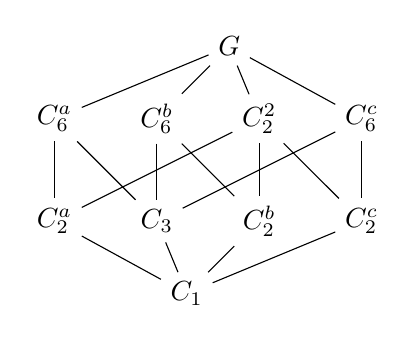
\begin{tikzpicture}[node distance=1.3cm]
        \node(G)[midway]{$G$};
        \node(C6b)[below left of =G]{$C_6^{b}$}; \node(C6a)[left of=C6b]{$C_6^{a}$};  
        \node(C22)[right of=C6b]{$C_2^{2}$};    \node(C6c)[right of=C22]{$C_6^{c}$};
        \node(C2a)[below of=C6a]{$C_2^{a}$};    \node(C3)[below of=C6b]{$C_3$};
        \node(C2b)[below of=C22]{$C_2^{b}$};    \node(C2c)[below of=C6c]{$C_2^{c}$};
        \node(C1)[below left of=C2b]{$C_1$};
        \draw(G)--(C6a);    \draw(G)--(C6b);    \draw(G)--(C6c);    \draw(G)--(C22);
        \draw(C6a)--(C2a);  \draw(C6a)--(C3);
        \draw(C6b)--(C2b);  \draw(C6b)--(C3);
        \draw(C6c)--(C2c);  \draw(C6c)--(C3);
        \draw(C22)--(C2a);  \draw(C22)--(C2b);  \draw(C22)--(C2c);
        \draw(C2a)--(C1);   \draw(C2b)--(C1);   \draw(C2c)--(C1);   \draw(C3)--(C1); 
    \end{tikzpicture}
    \end{figure}
    %There is a Brauer relation coming from the $C_2 \times C_2$-quotient, given by $$\Psi = C_3 - C_6^a - C_6^b - C_6^c + 2G.$$ 
    
    Consider an order $6$ character $\rho_a$ of $G$ with $C_2^{a}$ in its kernel. This has $\bQ(\rho_a) = \bQ(\zeta_6) = \bQ(\sqrt{-3})$. Let $\tau$ generate $\Gal(\bQ(\rho_a) / \bQ)$. One has
    \begin{equation}\label{ex1-rel}\tag{\textdagger}
    \Ind_{C_2^{a}}^G \trivial  \ominus \Ind_{C_6^{a}}^G \trivial \ominus \Ind_{C_2^{2}}^G \trivial \oplus \Ind_G^G \trivial \simeq \rho_a \oplus \rho_a^{\tau} .
    \end{equation}
    Let $E / \bQ$ be a semistable elliptic curve. To apply Theorem \ref{thm_positive_rank}, we need to compute
    \begin{equation}\label{ex1}\tag{*} 
        \frac{C_{E / F^{C_2^a}} C_{E / \bQ} }{C_{E / F^{C_6^a}} C_{E / F^{C_2^2}}} = 
        \frac{C_{E / L} C_{E / \bQ}}{C_{E / L^{C_3}} C_{E / L^{C_2}}}
    \end{equation} 
    where $L = F^{C_2^a}$ has $\Gal(L / \bQ) = C_6$, and check whether it is a norm from $\bQ(\sqrt{-3})$. This is a product of local Tamagawa numbers, as the minimal differential terms are $1$ when $E / \bQ$ is semistable (Lemma \ref{lem_Dterms}(i)). 
    
    One needs to compute these locally for each $p \in \bQ$. If $E / \bQ_p$ has good reduction, then the Tamagawa numbers at all places above $p$ in the subfields of $L$ are $1$. Suppose that $E / \bQ_p$ has split multiplicative reduction at $p$. Let $n = v_p(\Delta_E)$. For $H \leq G$, the Tamagawa number at a prime $\fP$ above $p$ in $L^H$ is given by $c_{\fp}(E / L^H) = e_{\fP \mid p} n$, where $e_{\fP \mid p}$ is the ramification degree. Thus the computation of Tamagawa numbers depends on the choice of decomposition group $D_p \leq C_6$ (to count the number of primes above $p$ in a given subfield) and the choice of inertia group $I_p \leq C_6$ (to compute the ramification indices). 
    
    The following table describes the product of Tamagawa numbers at places above $p$ in our expression, for varying $D_p$ and $I_p$. We let $T_{\fP \mid p}(E / L^H) = \prod_{\fP \mid p}c_{\fP}(E / L^H)$ for $H \leq \Gal(L / \bQ)$ as defined in Notation \ref{not_contr}. Let $C_p = c_p(E / \bQ)T_{\fP \mid p}(E / L) \big/ T_{\fP \mid p}(E / L^{C_3})T_{\fP \mid p}(E / L^{C_2})$. 
    \[
    \begin{array}{c c c c c c c}
        D_p & I_p & c_p(E / \bQ) & T_{\fP \mid p}(E / L^{C_3}) & T_{\fP \mid p}(E / L^{C_2}) & T_{\fP \mid p}(E / L) & C_p\\ 
        \hline
        C_1 & C_1 & n & n^2 & n^3 & n^6 & \square\\
        C_2 & C_1 & n & n & n^3 & n^3 & \square\\
        C_3 & C_1 & n & n^2 & n & n^2 & \square \\
        C_6 & C_1 & n & n & n & n & \square \\
        C_2 & C_2 & n & 2n & n^3 & (2n)^3 & \square \\
        C_6 & C_2 & n & 2n & n & 2n & \square \\
        C_3 & C_3 & n & n^2 & 3n & (3n)^2 & 3\cdot\square \\
        C_6 & C_3 & n & n & 3n & 3n & \square\\
        C_6 & C_6 & n & 2n & 3n & 6n & \square
    \end{array}
    \]

    In all cases we see that $C_p$, the contribution of Tamagawa numbers above $p$, is a norm form $\bQ(\sqrt{-3})$. It is not too hard to check that this is also the case when $E / \bQ_p$ has non-split multiplicative reduction. Therefore the expression in \eqref{ex1} is always a norm from $\bQ(\rho_a)$. This is an example of a more general phenomenon; for cyclic groups we always get a norm. This follows from  Theorem \ref{thm_consistent_cyclic}, which is proven in \S\ref{sec_cyclic}.
    %and $F / \bQ$ an abelian extension with $G = \Gal(F / \bQ)$. We claim that $C(\Theta) \in \fieldnorm{\rho_a}$, for all such $E$. Since each subgroup in $\Theta$ contains $C_2^{a}$, we have that $C(\Theta)$ equals $C(\Theta / C_2^{a})$ where $\Theta / C_2^{a} \in \B(G / C_2^{a}) = \B(C_6)$.  Now $\Theta / C_2^{a}$ is a $\chi_6$-relation, where $\chi_6 = \rho_a^{C_2^a}$ is a faithful order $6$ character of $C_6$, with $\bQ(\chi_6) = \bQ(\rho_a)$. But for cyclic groups we always get norm relations; by Theorem \ref{thm_consistent_cyclic}, $C(\Theta / C_2^{a}) \in \fieldnorm{\rho_a}$.

    But! Observe that{\footnote{this is called a Brauer relation, see Definition \ref{def-brauer}}} 
    \[ \Ind_{C_3}^G \trivial \ominus \Ind_{C_6^a}^G \trivial \ominus \Ind_{C_6^b}^G \trivial \ominus \Ind_{C_6^c}^G \trivial \oplus (\Ind_G^G \trivial)^{\oplus 2} = 0 \]
    as a virtual permutation representation. Append this to the left hand side of \eqref{ex1-rel}. Then Theorem \ref{thm_positive_rank} asks us to compute 
    \begin{equation}\label{ex1-rel2}\tag{**}
    \left(\frac{C_{E / F^{C_2^a}} C_{E / \bQ} }{C_{E / F^{C_6^a}} C_{E / F^{C_2^2}}}\right) \cdot \left( \frac{C_{E / F^{C_3}} C_{E / \bQ}^2}{C_{E / F^{C_6^a}}C_{E / F^{C_6^b}}  C_{E / F^{C_6^c}} } \right). 
    \end{equation}
    
    We can find instances where the second factor is not a norm from $\bQ(\sqrt{-3})$. Indeed suppose $E / \bQ$ has split multiplicative reduction at a prime $p$ with $D_p = G$, $I_p = C_6^b$. Let $v_p(\Delta_E) = n$. Then there is only one prime above $p$ in each subfield. Suppose $E$ has good reduction at all other primes (or multiplicative reduction at primes that are totally split in $F / \bQ$ would also be fine).
     Then our expression \eqref{ex1-rel2} is equal to
     \[ \frac{(6n)(n)}{(2n) (3n)} \cdot \frac{(2n)(n)^2}{(2n)(n)(2n)} \cdot \square = \frac{1}{2} \cdot \square, \] 
     which is not a norm from $\bQ(\sqrt{-3})$. Hence one must have $\rk E / F > 0$. 
\end{example}

\begin{example}[Dihedral]
    Let $q_1, q_2$ be odd primes. Consider $G = D_{2 q_1 q_2}$ the dihedral group of order $2 q_1 q_2$. 
    Let $\rho$, $\tau_1$, $\tau_2$ be two-dimensional irreducible representations of $G$ corresponding to rotating a $(q_1 q_2)$-gon by $2 \pi / q_1 q_2$, $2 \pi / q_1$, $2 \pi/ q_2$ respectively. These are all self-dual. The Galois conjugates of these representations, as well as the trivial $\trivial$ and sign $\epsilon$, yield all the irreducible representations of $G$. Let 
    \[  \sigma_{\rho} = \bigoplus_{ \fg \in \Gal(\bQ(\rho) / \bQ)} \rho^{\fg}, \qquad
        \sigma_1 = \bigoplus_{ \fg \in \Gal(\bQ(\tau_1) / \bQ)} \tau_1^{\fg}, \qquad
        \sigma_2 = \bigoplus_{ \fg \in \Gal(\bQ(\tau_2) / \bQ)} \tau_2^{\fg}. \]  
    Then $ \{ \trivial , \epsilon, \sigma_{\rho}, \sigma_1, \sigma_2 \}$ are a basis for the irreducible representations of $G$ over $\bQ$. 
    One has
\[
        \Ind_{C_2}^G \trivial \simeq \trivial \oplus \sigma_1 \oplus \sigma_2 \oplus \sigma_{\rho}, \quad
        \Ind_{D_{2 q_1}}^G \trivial \simeq \trivial \oplus \sigma_2, \quad
        \Ind_{D_{2 q_2}}^G \trivial \simeq \trivial \oplus \sigma_1,
\]
% There is an irreducible representation $\rho$ of $G$, obtained by inducing a linear order $q_1 q_2$ faithful representation from $C_{q_1 q_2}$. Thus $\rho$ is of degree $2$ and $\bQ(\rho) = \bQ(\zeta_{q_1 q_2})^{C_2}$. Then $\rho$ has $\frac{(q_1 - 1)(q_2 - 1)}{2}$ Galois conjugates, and so $\repnorm{\rho}$ is of dimension $2 \cdot \frac{(q_1 - 1)(q_2 - 1)}{2}$. 
and so 
\begin{equation*}
\Ind_{C_2}^G \trivial \ominus \Ind_{D_{2 q_1}}^G \trivial \ominus \Ind_{D_{2 q_2}}^G \trivial \oplus \Ind_{G}^G \trivial \simeq \bigoplus_{ \fg \in \Gal(\bQ(\rho) / \bQ)} \rho^{\fg}.
\end{equation*}

    Assume $E / \bQ$ is semistable. Suppose that $E / \bQ_p$ has split multiplicative reduction, with $n = v_p(\Delta_E)$. We compute Tamagawa numbers above $p$ as in the previous example, using the same notation. 
    Corollary \ref{cor-odd-decomp} implies that we always get a norm from the contribution above $p$ whenever the decomposition group is a group of odd-order. In fact we only get a non-square contribution when the decomposition group is $D_{2 q_1}$ or $D_{2 q_2}$ (and $I_p$ is non-trivial). 
     
    For example, let $p$ have decomposition group $D_{2 q_1}$ and inertia group $C_{q_1}$.
    This time, counting primes and computing ramification degrees is a little more awkward, we use Exercise \ref{ex-counting}.
        \begin{itemize}[--]
            \setlength\itemsep{0em}
            \item The action of $D_{2 q_1}$ on $C_2 \backslash G$ yields $1$ orbit of size $C_{q_1}$ (the orbit of the identity) and $\frac{q_2 - 1}{2}$ orbits of size $2q_1$ (coming from $C_2$ acting faithfully on $C_{q_2}$). The size of the inertia sub-orbits is $q_1$. Hence $T_{\fP \mid p}(E / F^{C_2}) = (q_1 n)^{1 + \frac{q_2 - 1}{2}}$.
            
            \item The action of $D_{2 q_1}$ on $D_{2 q_1} \backslash G$ yields the same number of orbits as above, but now the action of $C_{q_1} \leq D_{2 q_1}$ is trivial, so that $T_{\fP \mid p}(E / F^{D_{2 q_1}}) = n^{1 + \frac{q_2 - 1}{2}}$.
            
            \item The action of $D_{2 q_1}$ on $D_{2 q_2} \backslash G$ yields one orbit of size $q_1$, with the inertia sub-orbit also of size $q_1$, hence $T_{\fP \mid p}(E / F^{D_{2 q_2}}) = q_1 n$.
        \end{itemize}
    In total,
    \[ \frac{T_{\fP \mid p}(E / F^C_2) \cdot c_{\fp}(E / \bQ)}{T_{\fP \mid p}(E / F^{D_{2 q_1}})\cdot T_{\fP \mid p}(E / F^{D_{2 q_2}})} = \frac{(q_1 n )^{1 + \frac{q_2 - 1}{2}} (n)}{(n)^{1 + \frac{q_2 - 1}{2}} (q_1 n)} = q_1^{\frac{q_2 - 1}{2}} .\] 
    %By symmetry, taking the decomposition group to be $D_{2 q_2}$ and inertia group $C_{q_2}$, one would obtain $ q_2^{\frac{q_1 - 1}{2}}$.

    So let $E / \bQ$ have split multiplicative reduction at $p$ with decomposition group $D_{2 q_1}$ and inertia group $I_p = C_{q_1}$, and good reduction at all other primes. Further suppose that $q_1, q_2 \equiv 3 \pmod 4$ and that $\legendre{q_1}{q_2} = -1$. Then $\bQ(\sqrt{q_1 q_2}) \subset \bQ(\rho)$ but 
$$\frac{C_{E / F^C_2} C_{E / \bQ}}{C_{E / F^{D_{2 q_1}}} C_{E / F^{D_{2 q_2}}}} = q_1 \cdot \square$$
is not a norm from $\bQ(\sqrt{q_1 q_2})$. Indeed, $q_1$ is not the norm of an element of $\bQ(\sqrt{q_1 q_2})$, since $z^2 q_1 = x^2 - q_1q_2 y^2$ for $x,y,z \in \bZ$ implies $q_1 = \square \pmod {q_2}$, a contradiction. Thus $\rk E / F > 0$.

    This rank growth is predicted by root number computations also, however. Assume that $F / \bQ$ is totally real. Then $w(E / F^H) = (-1)^{[F^H \colon \bQ] + | H \backslash G / D_p|}$ by Proposition \ref{compute-root}. Thus
    \begin{itemize}[--]
        \setlength\itemsep{0em}
        \item $w(E / \bQ) = (-1)^2 = 1$,
        \item $w(E / F^{C_2}) = (-1)^{q_1 q_2} (-1)^{1 + \frac{q_2 - 1}{2}} = (-1)^{\frac{q_2 - 1}{2}}$,
        \item $w(E / F^{D_{2 q_1}}) = (-1)^{q_2}(-1)^{1 + \frac{q_2 - 1}{2}} = (-1)^{\frac{q_2 - 1}{2}},$
        \item $w(E / F^{D_{2 q_2}}) = (-1)^{q_1}(-1) = 1$. 
    \end{itemize}
    Therefore we must have $\rk E / F^{C_2}$, $\rk E / F^{D_{2q_1}} > 0$, so $\rk E / F > 0$. 
    Using the properties in Proposition \ref{compute-root-twist}, the computations of the root numbers for the subfields implies that 
    \[ w\left(E / \bQ, \sigma_1\right) = 1, \quad w\left(E / \bQ, \sigma_2\right) = -1, \quad w\left(E / \bQ, \sigma_{\rho}\right) = 1, \]
  and in particular $w(E / \bQ, \tau_1^{\fg}) = -1$ for some $\fg \in \Gal(\bQ(\tau_1) / \bQ)$.
\end{example}

\begin{example}[Additive reduction example]
Let $G = C_{65} \ltimes C_4$, where $C_4$ acts faithfully on $C_{65}$, as well as the subgroups $C_{13}$ and $C_5$. By inducing a faithful character of order $65$ from $C_{65}$, one obtains a faithful irreducible representation $\rho$ of $G$ of dimension $4$ and with $\bQ(\rho) = \bQ(\zeta_{65})^{C_4}$. In particular one has $\bQ(\sqrt{65}) \subset \bQ(\rho)$. Then
\[ \Ind_{C_4}^G \trivial \ominus \Ind_{C_{13} \ltimes C_4}^G \trivial \ominus \Ind_{C_5 \ltimes C_4}^G \trivial \oplus \Ind_{G}^G \trivial \simeq \bigoplus_{\fg \in \Gal(\bQ(\rho) / \bQ)} \rho^{\fg} .\]
Therefore by Theorem \ref{thm_positive_rank}, either 
\begin{equation}\label{ex3}\tag{\textdagger \textdagger}
\frac{C_{E / F^{C_4}} C_{E / \bQ} }{C_{E / F^{C_{13} \ltimes C_4}} C_{E / F^{C_5 \ltimes C_4}}}
\end{equation}
is a norm from $\bQ(\sqrt{65})$, or $\rk E / F > 0$.  

Suppose $p = 5$ and $E / \bQ_p$ has additive, potentially good reduction. Further suppose that $F / \bQ$ is an extension such that $D_{5} = I_{5} = C_5 \ltimes C_4$ (this is wildly ramified). Let $n = v_p(\Delta_E) < 12$. Then
\begin{itemize}[--]
    \setlength\itemsep{0em}
    \item In $F^{C_4}$ there is one prime above $p$ with ramification degree $5$ and $3$ primes above $p$ with ramification degree $20$,
    \item In $F^{C_{13} \ltimes C_4}$ there is one prime above $p$ with ramification degree degree $5$,
    \item In $F^{C_5 \ltimes C_4}$ there is one prime above $p$ with ramification degree $1$ and $3$ primes above $p$ with ramification degree $4$.
\end{itemize}
Therefore, by Lemma \ref{lem_Dterms}(iii), the product of the minimal differential term is 
\[ \frac{D_{\fP \mid p}(E / F^{C_4}) D_{\fP \mid p}(E / \bQ) }{D_{\fP \mid p}(E / F^{C_{13} \ltimes C_4}) D_{\fP \mid p}(E / F^{C_{5} \ltimes C_4})} = 
\frac{ 5^{\floor{5 n /12}} \cdot \left(5^{\floor{20 n /12}}\right)^3 }{5^{\floor{5 n /12}} \left(5^{\floor{4 n /12}}\right)^3} .\]
If $n = 2$, then this is equal to $5 \mod {(\bQ^{\times})^2}$. By Lemma \ref{tamagawa-num} the Tamagawa number product is
\[ \frac{T_{\fP \mid p}(E / F^{C_4}) T_{\fP \mid p}(E / \bQ) }{T_{\fP \mid p}(E / F^{C_{13} \ltimes C_4}) T_{\fP \mid p}(E / F^{C_{5} \ltimes C_4})} = \frac{1^2 \cdot 3^3 }{1^2 \cdot 3^3} = 1 \text{ or } \frac{1^5}{1^5} = 1.\]

We claim that $5$ is not a norm from $\bQ(\sqrt{65})$. Indeed, $5z^2 = x^2 - 65 y^2$ for $x, y, z \in \bZ$ implies that $5 = \square \pmod 13$, a contradiction since $\legendre{5}{13} = \legendre{13}{5} = \legendre{3}{5} = -1$. Therefore the local contribution of \eqref{ex3} above $5$ is not a norm from $\bQ(\sqrt{65})$. 

What are the local root numbers above $p$? By Proposition \ref{compute-root}, one has
\begin{itemize}[--]
    \setlength\itemsep{0em}
    \item $w(E / \bQ_5) = (-1)^{\floor{ 10 / 12}} = 1$, 
    \item $\prod_{\fp \mid p} w(E /F^{C_4}_{\fp}) = (-1)^{\floor{50 / 12}} \left((-1)^{\floor{200 / 12}}\right)^3 = 1$,
    \item $\prod_{\fp \mid p} w(E /F^{C_{13} \times C_4}_{\fp}) = (-1)^{\floor{50 / 12}} = 1$,
    \item $\prod_{\fp \mid p}w(E /F^{C_{5} \times C_4}_{\fp}) = (-1)^{\floor{ 10/12}}\left((-1)^{\floor{40 / 12}}\right)^3 = -1$ .
\end{itemize}
Hence we see a change in the contributions of local root numbers above $p$ in the intermediate subfields. 




\end{example}


\newpage
\section{Norm Relations}\label{sec_norm}
As observed in the introduction, we will be considering Artin representations over $\bQ$ that factor through finite Galois groups $G = \Gal(F / \bQ)$. Our methods in this report apply the theory of finite group representations to the study of elliptic curves over finite Galois extensions. This section introduces some representation-theoretic concepts that we will apply in later sections. 

The first two subsections discuss rational representations of $G$, and writing these as a sum of virtual permutation representations.
In the third subsection, we consider functions defined on subgroups of $G$, corresponding to subfields of $F / \bQ$. Our main example of interest is the function sending $H \mapsto C_{E / F^H}$ for $H \leq G$ \footnote{this is the fudge factor that appears in the BSD quotient for $E / F^H$}. We also describe \textit{$D$-local functions}, which are functions that depend on a decomposition group, borrowing definitions that appear in \cite[Section 2.iii]{reg-const}.

We have attempted to make this first section mainly representation-theoretic, in case the results within can be applied in other contexts.

\subsection{Rational characters and permutation representations}\label{rep}

\begin{defn} 
    Let $G$ be a finite group, $K$ a field of characteristic zero.
\begin{enumerate}
    \setlength\itemsep{0em}
    \item A \textbf{representation} of $G$ over $K$ is a group homomorphism $\rho \colon G \to \GL(V)$ where $V$ is a $K$-vector space.
    \item  Associated to a representation $\rho$ is a \textbf{character} $\chi \colon G \to K^{\times}$, defined by letting $\chi(g) = \Tr \rho(g)$ for $g \in G$. 
\end{enumerate}
\end{defn}

If we don't specify the field a representation is defined over, assume it is defined over $\bC$. For complex representations, $\rho$ is determined by its character; if $\rho$, $\rho'$ are representations with identical characters, then $\rho$ and $\rho'$ are isomorphic as representations (cf. \cite[Chapter 2, \S 2.3]{Serre}). 

%\begin{defn}\label{rep-ring}
%Let $\chi_1, \ldots,  \chi_h$ be the distinct characters of the complex irreducible representations of $G$, where $h = \#$ conjugacy classes of $G$. 
%Then the \textbf{representation ring} of $G$ is 
%\[ \R(G) = \bZ \chi_1 \oplus \cdots \oplus \bZ \chi_h .\]
%We can also view this as the Grothendieck group of the category of finitely generated $\bC[G]$-modules.
%\end{defn}
%Since we take differences of characters in $\R(G)$, we call elements of $\R(G)$ \textbf{virtual representations}. 

Let $K$ be a number field. Denote by $\R_K(G)$ the group generated by characters of the representations of $G$ over $K$. A representation of $G$ is then defined over $K$ if and only if its character is in $\R_K(G)$ {\color{red} ref Serre}.
$\R_K(G)$ is a subring of $\R_{\bC}(G)$, where $\R_{\bC}(G)$ is finitely generated by $\Irr(G)$; the irreducible characters of $G$ over $\bC$.
When $K = \bQ$ this is called the \textbf{rational representation ring}.
The characters of the distinct irreducible representations of $G$ over $K$ form an orthogonal basis of $\R_K(G)$ with respect to the usual inner product of characters of $G$ (\cite[Proposition 32]{Serre}).
Let $m$ be the exponent of $G$. If $K$ contains the $m$-th roots of unity, then $\R_K(G) = \R_{\bC}(G)$ (\cite[Theorem 24]{Serre}). This implies every representation of $G$ can be realized over such $K$. 
\vspace{1em}

%The rank of $R_K(G)$ is discussed in {\color{red} Serre 12.4}.
Let $\Perm(G)$ be the ring of virtual permutation representations of $G$ (i.e. the ring generated by the characters of $\bC[G / H] = \Ind_{H}^G \trivial$ for $H \leq G$). Let $\Char_{\bQ}(G)$ be the ring of rationally valued characters of $G$. Then we have inclusions 
\[ \Perm(G) \to \R_{\bQ}(G) \to \Char_{\bQ}(G). \]
Each of these groups have equal $\bZ$-rank, equal to the number of conjugacy classes of cyclic subgroups of $G$ (\cite[Chapter 13, \S13.1]{Serre}). Moreover the cokernels of these maps are finite.

\begin{defn}\label{rho-norm}
    Let $\rho$ be a representation of $G$. We define the norm of $\rho$, denoted $\repnorm{\rho}$, by 
    \[
    \repnorm{\rho} \defeq \sum_{\fg \in \Gal(\bQ(\rho)/\bQ)}  \rho^\fg \quad,
    \]
    where $\bQ(\rho)$ is the abelian extension of $\bQ$ generated by $\{ \Tr \rho(g) \colon g \in G \}$, and $\rho^\fg$ is the representation of $G$ such that $\Tr \rho^{\fg}(g) = \fg(\Tr \rho(g))$ for $g \in G$. 
\end{defn}

It's clear that $\Char_{\bQ}(G)$ is generated by the characters of $\repnorm{\rho}$ as $\rho$ ranges over the complex irreducible representations of $G$. Indeed, if a representation has a rationally valued character, then any complex irreducible constituent must occur along with all its Galois conjugates with equal multiplicity.

\begin{rem}
This is not additive, i.e. one does not have \[\repnorm{\rho + \tau} = \repnorm{\rho} + \repnorm{\tau}. \] 
This does hold when $\bQ(\rho) = \bQ(\tau)$. 
\end{rem}

\begin{example}
    Let $G = C_p$ and $\psi_p$ a character of order $p$. Then $\bQ(\psi_p) = \bQ(\zeta_p)$ and $\repnorm{\psi_p}$ is the sum over the $p - 1$ non-trivial characters of $G$. But $\repnorm{\psi_p + \trivial} = \trivial^{\oplus (p - 1)} + \repnorm{\psi_p} \not= \repnorm{\trivial} + \repnorm{\psi_p}$.
\end{example}

%Conversely,  Therefore our map $R(G) \to \Char_{\bQ}(G)$ is surjective.

%Such a character may not be in $R_{\bQ}(G)$, however. That is, it has rational character, but the corresponding representation cannot be realized over $\bQ$. The quotient $\Char_{\bQ}(G) / R_{\bQ}(G)$ is the study of Schur indices.  If $\rho \in R(G)$ is an irreducible representation, the \textbf{Schur index} is the smallest integer $m(\rho)$ such that 
%\[ \sum_{\sigma \in \Gal(\bQ(\rho)/\bQ)}m(\rho) \cdot \rho^\sigma \quad \in R_{\bQ}(G). \]

\begin{rem}\label{image-of-burnside}
The group $$\C(G) \defeq \frac{\Char_{\bQ}(G)}{\Perm(G)}$$ is a finite abelian group, of exponent dividing $|G|$ (this follows from Artin's induction theorem {\color{red} ref}). The study of this group is quite subtle. For us, it's enough to know that given a representation $\rho$ of $G$, there exists a minimum integer $m$, depending on $\rho$ and dividing $|G|$, such that 
\[ \repnorm{\rho}^{\ \oplus m } = \bigoplus_i \Ind_{H_i}^G \trivial \ominus \bigoplus_j \Ind_{H_j'}^{G} \trivial \]
for some subgroups $H_i$, $H_j' \leq G$, i.e. that the character of $\repnorm{\rho}^{\ \oplus m }$ is in $\Perm(G)$. This minimum integer $m$ is the order of the character of $\repnorm{\rho}$ in $\C(G)$. 
\end{rem}
%Thus, we have a map $\Irr(G) \to \Perm(G)$. We extend this additively to a map $R(G) \to \Perm(G)$.
\begin{example}
If $G = C_n$ then $\C(G)$ is trivial (see Example \ref{cyclic-relns}). $\C(G)$ is also trivial for the symmetric groups $G = S_n$. 
\end{example}

 \begin{example}
    $G = Q_8$, the quaternion group, has $\C(G) = \bZ / 2 \bZ$. Let $\rho$ be the faithful irreducible representation of $G$ of dimension $2$. Its character $\chi$ is rational and one has 
    \[ \rho^{\oplus 2} = \Ind_{C_1}^G \trivial \ominus \Ind_{C_2}^G \trivial, \]
    but one cannot write $\rho$ as a virtual permutation representation ($\chi$ has Schur index $2$ so $\chi \not\in \R_{\bQ}(G)$).  
 \end{example}

%\begin{notn}
%For $\rho \in R_{\bC}(G)$ an irreducible character let 
%\[  \repnorm{\rho} = \sum_{\sigma \in \Gal(\bQ(\rho)/\bQ)}m(\rho)\cdot \rho^\sigma \quad \in R_{\bQ}(G) , \]
%where $m(\rho) \in \bZ$ is the Schur index of $\rho$.
%\end{notn}
%Then $\repnorm{\rho}$ is the character of an irreducible rational representation. Every irreducible rational representation can be obtained this way. We can extend this map additively to a surjective map $R_{\bC}(G) \to R_{\bQ}(G)$. 

%Let $\overline{R_K(G)}$ be the subring of elements of $R(G)$ which have values in $K$. Then $R_K(G) \subset \overline{R_K(G)}$ and this inclusion is of finite index. 
%Given a character $\chi$ of $G$, let $\bQ(\chi)$ be the smallest subfield of $\bC$ containing $\{ \chi(g) \mid g \in G \}$.
%Let $R_{\bC}(G)$ denote the ring of characters of complex representations of $G$. The number of complex irreducible representations of $G$ is equal to the number of conjugacy classes of $G$. Let $R_{\bQ}(G)$ be the ring of characters of rational valued representations of $G$.
%The number of irreducible $\bQ G$-representations up to isomorphism is equal to the number of conjugacy classes of cyclic subgroups of $G$. %(\cite[$\mathsection 13.1$, Cor. 1]{Serre})
%Induction, Restriction\dots
%\begin{thm}[Mackey Decomposition] 
%\end{thm} 
\subsection{The Burnside ring and relations for permutation representations}

Let $G$ be a finite group. Recall that there is a bijection  
\[ \{ \text{transitive finite }G\text{-sets } X  \text{ up to isomorphism}\}\leftrightarrow  \{ \text{subgroups } H \leq G \text{ up to conjugacy} \} \] 
given by sending a transitive finite $G$-set $X$ to $H = \Stab_{G}(x)$ for some $x \in X$.  The action of $G$ on $X$ is equivalent to the action of $G$ on $G / H$. 

\begin{defn}\label{burnside}
Let $[X]$ denote the isomorphism class of a $G$-set $X$. 
The \textbf{Burnside ring} $\B(G)$ is the free abelian group on isomorphism classes of finite $G$-sets, modulo the relations  $[S] + [T] = [S \sqcup T]$ for $S$, $T$ finite $G$-sets. This is a ring; multiplication is given by $[S] \cdot [T] = [S \times T]$.
\end{defn}

We only need that $\B(G)$ is a group, and do not use its multiplicative structure. $\B(G)$ is generated by $\{ [X] \colon X \text{ finite transitive } G\text{-set}\}$. Using the identification of finite transitive $G$-sets with subgroups of $G$, we write elements of $\B(G)$ as $\sum_i n_i H_i$ for $n_i \in \bZ$, $H_i \leq G$. 

\begin{defn}
    Given a $G$-set $X$, one obtains a representation of $G$ by considering its permutation representation $\bC[X]$. We extend this to $\B(G)$; given $\Theta  = \sum_i n_i H_i \in \B(G)$, define 
    \[ \bC[G / \Theta ] = \sum_i n_i \Ind_{H_i}^G \trivial. \]
    Let $\chi_{\bC[G / \Theta]}$ be the character of $\bC[G / \Theta]$. Then  $\Theta \mapsto \chi_{\bC[G / \Theta]}$ defines a homomorphism $\B(G) \to \Perm(G)$.
\end{defn}

\begin{defn}
If $\bC[G / \Theta] = 0$ as a virtual permutation representation (i.e. $\chi_{\bC[G / \Theta]} = 0$), then $\Theta$ is called a  \textbf{Brauer relation}.
\end{defn}

Non-trivial Brauer relations are instances of non-isomorphic $G$-sets giving rise to isomorphic permutation representations. 

\begin{example}
    The irreducible representations of $G = S_3$ are the trivial representation $\trivial$, the sign representation $\epsilon$ and the $2$-dimensional representation $\rho$.
    We have
    \begin{table}[H]
        \centering
    \begin{tabular}{l l l l l l l}
        $\bC[G / C_1]$ & $=$ & $\trivial \oplus \epsilon \oplus \rho^{\oplus 2},$ & $\qquad$ &
        $\bC[G / C_2]$ & $=$ & $\trivial \oplus \rho,$\\ 
        $\bC[G / C_3]$ & $=$ & $\trivial \oplus \epsilon,$ & $\qquad$ &
        $\bC[G / G]$ & $=$ & $\trivial.$  
    \end{tabular}
\end{table}
    Then $\Psi = C_1  - 2 C_2 - C_3 + 2S_3$ is the unique Brauer relation for $G$.
\end{example}

\begin{example}\label{cyclic-no-brauer}
Cyclic groups have no Brauer relations. Indeed, if $G = C_n$, the $\bZ$-rank of $\Perm(G)$ is the number of cyclic subgroups of $C_n$, i.e the number of subgroups of $C_n$, which is the $\bZ$-rank of $\B(G)$. Hence the rank of the kernel of the map $\B(G) \to \Perm(G)$ is zero.
\end{example}

In the last section, we described how to obtain a virtual permutation representation from an arbitrary representation of $G$. We are interested in when this is an image of an element from the Burnside ring.

\begin{defn}
Let $\rho$ be a representation of $G$.    
We call $\Theta = \sum_i n_i H_i \in \B(G)$ a \textbf{$\rho$-relation} if $\bC[G / \Theta] \simeq \repnorm{\rho}^{\ \oplus m}$, for some $m \geq 1$.
\end{defn}

If $D \leq G$, then one can pass from virtual permutation representations of $G$ to virtual permutation representations of $D$ via restriction, and in the other direction via induction. We define analogous maps for the Burnside ring.    

\begin{defn}
    For $D \leq G$, define maps $\Res_D \colon \B(G) \to \B(D)$ and $\Ind_D \colon \B(D) \to \B(G)$ by
    \[  \Res_D H = \sum_{x \in H \backslash G / D} D \cap H^{x^{-1}}, \qquad \quad \Ind_D H = H. \]
    These correspond to the representation theory side, where $\Res_D \Ind_{H}^G \trivial = \sum_{x \in H \backslash G / D} \Ind_{D \cap H^{x^{-1}}}^D \trivial$ (Mackey's decomposition, cf. \cite[Chapter 7, \S 7.3]{Serre}, $H^{x^{-1}} = x^{-1}H x$), and $\Ind_{D}^G\Ind_{H}^D \trivial = \Ind_{H}^G \trivial$.
\end{defn}
%\begin{rem}
%If such a relation exists, then $m$ is a multiple of the order of $\repnorm{\rho}$ in $C(G)$. Note that if $\Theta$ is a $\rho$-relation and $\Psi \in B(G)$ is a Brauer relation, then $\Theta + \Psi$ is also a $\rho$-relation. It follows that for a fixed $m \geq 1$, if $\repnorm{\rho}^{\oplus m} \in \Perm(G)$ then there are $\#$(Brauer relations of $G$) $+ 1$ elements $\Theta \in \B(G)$ with $\bC[G / \Theta] = \repnorm{\rho}^{\oplus m}$.
%\end{rem}

The following are some elementary properties of these relations:

\begin{prop} Let $\rho$ be a representation of $G$, $\Theta = \sum_i n_i H_i \in \B(G)$ a $\rho$-relation. Then,
    \begin{enumerate}
        \item $n \Theta$ is a $\rho$-relation for all $n \geq 1$.
        \item $\bC[G / \Theta] \simeq \repnorm{\rho}^{\oplus m}$ where $m$ is a multiple of the order of the character of $\repnorm{\rho}$ in $\C(G)$.
        \item If $\Psi \in B(G)$ is a Brauer relation, then $\Theta + \Psi$ is also a $\rho$-relation. 
        \item For a fixed $m \geq 1$, if $\repnorm{\rho}^{\oplus m}$ is a virtual permutation representation then there are $\#$(Brauer relations of $G$) $+ 1$ elements $\Theta \in \B(G)$ with $\bC[G / \Theta] = \repnorm{\rho}^{\oplus m}$.
        
        \item (Projection) If $N \trianglelefteq G$ then $(N \cdot \Theta) / N = \sum_i n_i N H_i / N$ is a $\rho^N$-relation, viewing this relation as an isomorphism of representations of $G / N$.
        \item (Restriction) For $D \leq G$, $\Res_D \Theta$ is a $\Res_D \rho$-relation.
    \end{enumerate}
\end{prop}

\begin{proof}
    All but (5) are clear. For (5), observe that for $H \leq G$, $\bC[G / H]^N \simeq \bC[G / NH]$ as $G$-representations (see proof of \cite[Theorem 2.8]{reg-const}). We also need to show that $\repnorm{\rho}^N \simeq \repnorm{\rho^N}^{\oplus k}$ for some $k \geq 1$. This is the case; 
    $$\repnorm{\rho}^N = \left(\bigoplus_{\fg \in \Gal(\bQ(\rho) / \bQ)} \rho^{\fg} \right)^N \simeq 
    \bigoplus_{\fg \in \Gal(\bQ(\rho) / \bQ)} (\rho^{\fg})^N \simeq \bigoplus_{\fg \in \Gal(\bQ(\rho) / \bQ)} (\rho^N)^{\fg} = \repnorm{\rho^N}^{\oplus k},$$
    where $k = [ \bQ(\rho) : \bQ(\rho^N)]$. 
\end{proof}


\begin{example}\label{cyclic-relns}[\cite[Exercise 13.1]{Serre}]
    Let $G = C_n$. For each $d \mid n$, let $\chi_d = \repnorm{\varphi_d}$, where $\varphi_d$ is an irreducible complex character of $G$ with field of values $\bQ(\zeta_d)$ and kernel of index $d$.
    Then $\{ \chi_d \colon d\mid n \}$ form an orthogonal basis for the irreducible rational-valued representations of $G$. Since $C_{n / d} \trianglelefteq G$, $\Ind_{C_{n/ d}}^G \trivial$ is the direct sum of irreducible complex representations of $G$ containing $C_{n / d}$ in their kernel. Thus, $\Ind_{C_{n/ d}}^G \trivial \simeq \sum_{d' \mid d} \chi_{d'}$. Applying M\"{o}bius inversion, we obtain a $\varphi_d$-relation for each $d \mid n$:
    \[ \chi_d = \sum_{d' \mid d} \mu(d / d') \cdot \Ind_{C_{n/ d}}^G \trivial. \]
    Note that this is the only way of writing $\chi_d$ as a sum of permutation representations, since cyclic groups have no Brauer relations (Example \ref{cyclic-no-brauer}). Similarly, there is a unique $\Theta \in B(G)$ such that $\bC[G / \Theta] \simeq \chi_d^{m}$ for all $m \geq 1$.
    \end{example}

\subsection{Functions on the Burnside ring and norm relations}\label{sec-norm-rels}

Let $f \colon \B(G) \to A$ be a multiplicative function with $f(\sum_i n_i H_i) = \prod_i f(H_i)^{n_i}$ where $A$ is an abelian group. As in \cite{reg-const}, we say that $f$ is \textbf{representation theoretic} if $f$ is trivial on Brauer relations. This implies that for a $G$-set $X$, $f$ only depends on the representation $\bC[X]$. 
%In other words, there exists a map $g \colon \R(G) \to A$ such that $f(H) = g(\bC[G / H])$ for all $H \leq G$. 

\begin{example}
  Let $\lambda \in \bR^{\times}$ and consider the function $H \mapsto \lambda^{[G : H]}$. This is trivial on Brauer relations;  if $\sum_i n_i H_i$ is a Brauer relation then $\lambda^{\sum_i n_i [G : H]} = \lambda^{\dim( \oplus_i \bC[G / H_i]^{\oplus n_i})} = 1$.
\end{example}

Let $\rho \in \R(G)$. Let $\Theta \in \B(G)$ be a $\rho$-relation, with $\bC[G / \Theta] \simeq \repnorm{\rho}^{\oplus m}$. If we have a function $f \colon \B(G) \to \bQ^{\times}$, we may then ask whether $f(\Theta) \in \fieldnorm{\rho}$. 

%Take a multiplicative function on the Burnside ring of the form $\psi \colon \B(G) \to \bQ^{\times}$. Given $\rho \in R_{\bC}(G)$ we can extend such functions from the Burnside ring to $\overline{\psi} \colon \B(G) \to \bQ^{\times} /\fieldnorm{\rho}$. {\color{red} motivate this a bit better?}

\begin{defn}
Let $\rho \in \R(G)$, $\Theta$ a $\rho$-relation, and $f \colon \B(G) \to \bQ^{\times}$. If $f(\Theta) \in \fieldnorm{\rho}$, then we call $\Theta$ a \textbf{norm relation} for $f$. 
If $f(\Theta) \in \fieldnorm{\rho}$ for every $\rho$-relation in $\B(G)$, then we say $f$ is \textbf{trivial on $\rho$-relations}.

    %If $\Theta \in \ker \overline{\psi}$, then $\psi(\Theta)$ is the norm of an element from $\bQ(\rho)^{\times}$. We call an instance of this a \textbf{norm relation}.
\end{defn}

%\begin{defn}
% We say two functions $\psi$, $\psi'$ are \textbf{$\rho$-equivalent}, written $\psi \sim_{\rho} \psi'$, if $\overline{\psi /\psi'}$ is trivial on all $\rho$-relations. Equivalently, $\psi(\Theta) / \psi'(\Theta)$ is a norm relation for all $\rho$-relations $\Theta$. 
%\end{defn}

%If a function $f$ satisfies $f \sim_{\rho} 1$, we say $f$ is trivial on $\rho$-relations. 

\begin{example}
    Let $G = C_p$ for $p$ a prime. Let $\rho$ be a character of degree $p$, so $\bQ(\rho) = \bQ(\zeta_p)$. There is a unique $\rho$-relation given by $\Theta = C_1 - C_p$. Let $\psi \colon \B(G) \to \bQ^{\times}$ be given by $\psi(H) = [G \colon H]$. Then $\psi(\Theta)$ is a norm relation, as $\psi(\Theta) = p \in \fieldnorm{\rho}$ is the norm of $1 - \zeta_p$.
\end{example}

In general, showing that a $\rho$-relation $\Theta$ is a norm relation for $f$ does not imply that this is the case for all possible $\rho$-relations. Under certain circumstances however, we can.

\begin{prop}\label{min-to-all}
    Let $\rho \in \R(G)$ and $f \colon \B(G) \to \bQ^{\times}$. Suppose that $f(\Psi) \in \fieldnorm{\rho}$ for every Brauer relation $\Psi \in \B(G)$. 
    Let $\Theta \in \B(G)$ be a $\rho$-relation, with $\bC[G / \Theta] = \repnorm{\rho}^{\oplus m}$, where $m$ is the order of $\repnorm{\rho}$ in $\C(G)$. 
    If $\Theta$ is a norm relation for $f$, then $f$ is trivial on $\rho$-relations. 
\end{prop}

\begin{proof}
    Consider an arbitrary $\rho$-relation $\Theta'$ such that $\bC[G / \Theta'] = \repnorm{\rho}^{\oplus l}$ for some $l \geq 1$. Then $m \mid l$ and $\Psi = \Theta' - \frac{l}{m}\Theta$ is a Brauer relation. Thus
    \[ f(\Theta') = f(\Psi)\cdot f(\Theta)^{\frac{l}{m}} \in \fieldnorm{\rho} \]
    and so $f$ is trivial on all $\rho$-relations.
\end{proof}

\begin{example}
    Let $G = C_n$. Then any function $f \colon \B(G) \to \bQ^{\times}$ is trivial on Brauer relations since $G$ does not have any. Let $\varphi_d$ be an irreducible complex character of $G$ of order $d \mid n$. Thus to conclude that $f$ is trivial on $\varphi_d$-relations, it is enough to show that the $\varphi_d$-relation constructed in Example \ref{cyclic-relns} is a norm relation for $f$.
\end{example}

%\begin{example}
%Let $\bQ(\rho)$ be a quadratic field. Then if $f \colon \B(G) \to \bQ^{\times}$ satisfies $f(\Theta) \in \bQ^{\times 2}$ for all $\rho$-relations $\Theta$, one has $f \sim_{\rho} 1$.
%\end{example}

\begin{example}
Let $E / \bQ$ be an elliptic curve, $G = \Gal(F / \bQ)$ for $F / \bQ$ a Galois extension. The function $C \colon H \mapsto C_{E / F^H}$ ({\color{red} ref}) for $H \leq G$ extends to a multiplicative function on the Burnside ring. In later sections we will investigate when this is trivial on $\rho$-relations, for $\rho \in \R(G)$. 
\end{example}

It appears quite difficult in general to describe the set of $\rho$-relations for some finite group $G$ and $\rho \in \R(G)$. Thus determining functions that are trivial on $\rho$-relations is even more difficult. We have a better understanding of the relations when $G$ is cyclic, and can prove the following result.

\begin{prop}\label{index-fn-trivial}
    Let $G = C_n$. Let $\rho \in \R(G)$ such that $[\bQ(\rho) \colon \bQ] = 2$. Consider the function $g \colon \B(G) \to \bQ^{\times}$ given by $H \mapsto [G : H]$. Then $g$ is trivial on $\rho$-relations.
\end{prop}

\begin{proof}
    Let $\ff$ be the minimum positive integer such that $\bQ(\rho) \subset \bQ(\zeta_{\ff})$. As $\bQ(\rho)$ is quadratic, $\ff$ is described in Remark \ref{conductor} (it is the absolute value of the discriminant $\Delta$ of $\bQ(\rho)$). Observe that $\ff \mid n$ since all characters of $G$ are realized over $\bQ(\zeta_n)$. Since $\C(G) = 1$ and $G$ has no Brauer relations, by Proposition \ref{min-to-all} it suffices to show that $\Theta \in \fieldnorm{\rho}$ for $\Theta \in \B(G)$ such that $\bC[G / \Theta] = \repnorm{\rho}$.


    Let $\repnorm{\rho} = \sum_{d \mid n} a_d \chi_d$ where $a_d \in \bZ$ and $\chi_d$ are the basis of irreducible rational representations of $C_n$ defined in Example \ref{cyclic-relns}. %(recall $\chi_{d} = \repnorm{\varphi_{d}}$ with $\bQ(\varphi_{d}) = \bQ(\zeta_{d})$ form a basis for the irreducible rational representations of $C_n$). 
    Let $\Psi_{d} = \sum_{d' | d}\mu(d / d')\cdot C_{n / d}$ so that $\bC[\Psi_{d}] = \chi_{d}$, as observed in the example. Then $\bC[G / \Theta] \simeq \bC[\sum_{d | n } a_{d} \Psi_{d}]$ which implies that $\Theta = \sum_{d | n } a_{d} \Psi_{d}$.

    Evaluating $g$ on $\Psi_{d}$ is trivial unless $d = q^a$ for some $q$ prime, $a \geq 1$. Indeed, if $d = p_1^{e_1} \cdots p_r^{e_r}$ , with $r \geq 2$ and $e_i \geq 1$, then
    \[ \prod_{d' \mid d} (d')^{\mu(d / d')} = \prod_{j_1, \ldots j_r \in \{0,1\}^r } \left(p_1^{e_1 - j_1} \cdots p_r^{e_r - j_r}\right)^{\# j_i = 1} = \prod_{i = 1}^r \left(\frac{p_i^{e_i}}{p_i^{e_i - 1}}\right)^{\sum_{ j = 0}^{r - 1} \binom{r-1}{j} (-1)^j} = 1. \]
    On the other hand,
    \[ \prod_{d' \mid q^a} (d')^{\mu(q^a / d')} = q .\]
    
    The irreducible representations of $C_n$ over $\bQ(\rho)$ are given by the orbits of the complex irreducible characters of $C_n$ acted upon by $H = \Gal (\bQ(\zeta_n) / \bQ(\rho))$. Consider $d \mid n$ with $\ff \nmid d$, so that $\bQ(\rho) \not\subset \bQ(\zeta_d)$. 
    Recall that $\chi_d = \repnorm{\varphi_d}$, where $\bQ(\varphi_d) = \bQ(\zeta_d)$. Let $B = \Gal(\bQ(\zeta_n) / \bQ(\zeta_d))$. Then $\bQ(\rho) \cap \bQ(\zeta_d) = \bQ$, so $BH = \Gal(\bQ(\zeta_n) / \bQ)$. The orbit of $\varphi_{d}$ under $H$ is fixed by $BH$, hence is rational. It follows that $\langle \rho, \varphi_{d} \rangle = \langle \rho^{\sigma} , \varphi_{d} \rangle$ for $\sigma$ the generator of $\Gal(\bQ(\rho) / \bQ)$. Thus $2 = [\bQ(\rho) : \bQ]$ divides $a_d$, and so $g(a_d \Psi_d) = g(\Psi_d)^{a_d} \in \bQ^{\times 2} \subset \fieldnorm{\rho}$.

    Thus $a_d$ can only be odd when $\ff \mid d$. Therefore for $g(\Theta)$ to be non-square we require $\ff = p$ for some prime $p$. Then $p$ must be odd ($|\Delta|$ cannot be $2$) and $\bQ(\rho) = \bQ(\sqrt{p^*})$. But $p$ is a norm in $\bQ(\sqrt{p^*})$ by Corollary \ref{p-norm}.
\end{proof}

\subsubsection{D-local functions}\label{D-loc}

We are interested in functions on the Burnside ring that are number-theoretic in nature, where we take $G$ to be a Galois group. Often, these functions are \textit{local}. 

\begin{example}
Let $F / K$ be a finite Galois extension of number fields and let $G = \Gal(F / K)$. Let $\fp$ be a prime of $K$ and $\fq$ a prime of $F$ above $\fp$. Let $D_{\fq} \leq G$ be the corresponding decomposition group. For $H \leq G$, the number of primes in $L = F^{H} = K(\alpha)$ above $\fp$ are in one-to-one correspondence with the double cosets $H \backslash G / D_{\fq}$. This correspondence is given by sending a prime $\fs$ in $L$ above $\fp$ to the elements of $G$ that send $\fq$ to some prime above $\fs$.

We can use the function $f \colon \B(G) \to \bQ^{\times}$ given by $H \mapsto  \lambda^{| H \backslash G / D|}$ (for $\lambda \not= \pm 1$) to describe the number of places above $\fp$ in any intermediate extension of $F / K$. But if we let $g \colon \B(D) \to \bQ^{\times}$ be defined by $H \mapsto \lambda$, then 
        \[ f(H) = g\left(\Res_D H\right) = \prod_{x \in H \backslash G / D} g(D \cap H^{x^{-1}}) .\]
Therefore the value of $f$ on any $G$-set $X$ only depends on the structure of $X$ as a $D$-set.
\end{example}

Such functions motivate the following definition:

\begin{defn}(\cite[Definition 2.33]{reg-const})\label{D-loc-fn}
    If $D \leq G$, we say a function $f$ on $\B(G)$ is \textbf{$D$-local} if there is a function $f_D$ on $\B(D)$ such that $f(H) = f_D(\Res_D H)$ for $H \leq G$.
    If this is the case, we write
    \[ f = (D, f_D). \]
\end{defn}

\begin{example}\label{tama-ex}
    For $G = \Gal(F / K)$, $v$ a place of $K$ with decomposition group $D$, the function
    \[ H \mapsto \prod_{w | v} c_w(E / F^{H}) \]
    is $D$-local, where $E$ is an elliptic curve over $K$ and $c_w$ is the local Tamagawa number. 
\end{example}

Let $I \triangleleft D$ be the inertia subgroup of the place $v$, so $D / I$ is cyclic. If a prime $w$ in $F^H$ corresponds to the double coset $HxD$, then its decomposition and inertia groups in $F / F^H$ are $H \cap D^x$ and $H \cap I^x$ respectively.
The ramification degree and residue degree of $w$ over $K$ are given by $e_w = \frac{|I|}{|H \cap I^x|}$ and $f_w = \frac{[D : I]}{[H \cap D^x : H \cap I^x]}$. We will consider functions that depend on $e$ and $f$, and so introduce the following:

\begin{defn}\cite[Definition 2.35]{reg-const}\label{D-I-fn}
    Suppose $I \triangleleft D < G$ with $D / I$ cyclic, and $\psi(e,f)$ is a function of $e, f \in \bN$. Define a function on $\B(G)$ by 
    \[ \left(D, I, \psi\right) \colon \quad H \mapsto \prod_{x \in H\backslash G / D} \psi\left(\frac{|I|}{|H \cap I^x|}, \frac{[D : I]}{[H \cap D^x : H \cap I^x]}\right). \]
    This is a $D$-local function on $\B(G)$ with
    \[ (D, I, \psi) = \left(D, U \mapsto \psi\left(\frac{|I|}{|U \cap I|}, \frac{|D|}{|UI|}\right)\right). \]
\end{defn}

\begin{example}
    If $E / K$ has split multiplicative reduction at $v$ with $c_v(E / K) = n$, then $c_w(E / F^H) = e_w n$ for a place $w$ of $F^H$ above $v$. In this case the function in Example \ref{tama-ex} is $(D, I, e n)$. 
\end{example}

%\begin{example}\label{trivial-on-brauer}
%    Let $\rho = 0$. If $W$ is a group of odd order, then $(W, W, e) \sim 1$ as functions to $\bQ^{\times} / \bQ^{\times 2}$.More generally if $D$ has odd order and $I \triangleleft D$ then $(D, I, e) \sim_{\rho} 1$. {\color{red} explain and reference}
%\end{example}

\begin{prop}
    Let $D \leq G$, $N \trianglelefteq G$. Let $\rho \in \R(G)$.
%    {\color{red} these aren't right... i need to consider the fields...}
%    Let $I \triangleleft D \leq G$ with $D / I$ cyclic. Let $\rho \in \R(G)$ Then
    \begin{enumerate}
        \item (Restriction) Suppose that $\bQ(\rho) = \bQ(\Res_D \rho)$. If $f = (D, f_D)$ and $f_D$ is trivial on $(\Res_D \rho)$-relations, then $f$ is trivial on $\rho$-relations.
        \item (Projection) Suppose that $\bQ(\rho) = \bQ(\rho^N)$ (view $\rho^N$ as a representation of $G / N$). Consider $f$ a function on $\B(G)$ such that $f(H) = f_{G / N}(N H / N)$ for some function $f_{G / N}$ on $\B(G / N)$. If $f_{G / N}$ is trivial on $\rho^N$-relations (viewed in $\R(G / N)$ ), then $f$ is trivial on $\rho$-relations.
    \end{enumerate}
\end{prop}

 One would like to be able to say that if $f = (D, f_D)$ and $f_D$ is trivial on $(\Res_D \rho)$-relations, then $f$ is trivial on $\rho$-relations. But as defined, one cannot conclude this when $[\bQ(\rho) : \bQ(\Res_D \rho) ] > 1$. Under some conditions however, when $\bQ(\Res_D \rho) = \bQ$, one can automatically conclude that $f$ is trivial on $\rho$-relations, as in the following.

\begin{prop}\label{rational-res}
Let $D \leq G$. Consider $\rho \in \R(G)$ with $[\bQ(\rho) : \bQ] = n$, where multiplication by $n$ is injective on $\C(D)$. Consider $f = (D, f_D)$ a $D$-local function on $\B(G)$. 
Suppose that $f_D(\Psi) \in \fieldnorm{\rho}$ for every Brauer relation $\Psi \in \B(D)$.
Then, if $\bQ(\Res_D \rho) = \bQ$, $f$ is trivial on $\rho$-relations.
%\colon \B(G) \bQ^{\times}$ a $D$-local function be a function that is trivial on Brauer relations. We also show that if $\bQ(\Res_{D_p} \rho) = \bQ$, then $(T_{\fP \mid p} \cdot D_{\fP \mid p})(\Theta) \in \bQ^{\times 2}$.
\end{prop}

\begin{proof}
    Let $\Theta$ be a $\rho$-relation, with $\bC[G / \Theta] \simeq \repnorm{\rho}^{\oplus m}$. Then $$\bC[D / \Res_D \Theta] \simeq \repnorm{\Res_D \rho}^{\oplus m n} \in \Perm(D).$$ 
    The condition on $n$ ensures that there exists $\Theta' \in \B(D)$ with $\bC[D / \Theta'] \simeq \repnorm{\Res_D \rho}^{\oplus m} \in \Perm(D).$ Then $\Psi = \Res_D\Theta - n\Theta'$ is a Brauer relation for $D$. Thus
    \[ f(\Theta) = f_D(\Res_D \Theta) = f_D(\Psi)f_D(n\Theta') = f_D(\Psi)f_D(\Theta')^n \in \fieldnorm{\rho}, \]
    since $f_D(\Psi) \in \fieldnorm{\rho}$ and $\bQ^{\times n} \subset \fieldnorm{\rho}$. 
\end{proof}

The following is an example of when constant $D$-local functions are squares when evaluated on $\rho$-relations.

\begin{prop}\label{const-fns}
     Let $D \leq G$ with $D$ of odd order, and $f = (D, \alpha)$ a $D$-local function on $\B(G)$, where $\alpha \in \bQ^{\times}$ is constant. Let $\rho \in \R(G)$ with $[\bQ(\rho) : \bQ ]$ even. Then for a $\rho$-relation $\Theta$, $f(\Theta) \in \bQ^{\times 2}$. 
\end{prop}

\begin{proof}
    The function $(D, \alpha)$ on $\B(G)$ sends $H \leq G$ to $\alpha^{| H \backslash G / D|}$. Let $\Theta = \sum_i n_i H_i$ be a $\rho$-relation with $\bC[G / \Theta] \simeq \repnorm{\rho}^{\oplus m}$ for some $m \geq 1$. One has $(D, \alpha)(\Theta) = \alpha^{\sum_i n_i \cdot | H_i \backslash G / D|}$. We show that $\sum_i n_i \cdot | H_i \backslash G / D |$ is even.

    One has $\Res_D \Theta = \sum_i n_i \sum_{x \in H_i \backslash G / D} D \cap H_i^{x^{-1}}$, and $\bC[D / \Res_D \Theta]$ has even dimension, since it is isomorphic to $\sum_{\Gal(\bQ(\rho) / \bQ)} \Res_D \rho^{\sigma}$ and $\Gal(\bQ(\rho) / \bQ)$ has even order. The dimension is $$\sum_i n_i \sum_{x \in H_i \backslash G / D} [D : D \cap H_i^{x^{-1}} ].$$ Since each $[D : D \cap H_i^{x^{-1}} ]$ is odd, this implies there are an even number of terms in the summation, i.e. that $\sum_i n_i \cdot | H_i \backslash G / D|$ is even. 

\end{proof}

%Our fudge factors $C(E / F)$ are defined locally; one has $C(E / F) = \prod_v c_v(E / F) \cdot |\omega / \omega_{v, \min}|$. Here $v$ runs over finite places of $F$, $\omega$ is a global minimal differential for $E / \bQ$, and $\omega_{v, \min}$ is a minimal differential at $v$.
%Considering the function $H \mapsto C(E / F^H)$, and writing $C_p(E / F^H) =\prod_{v | p} c_v(E / F)\cdot |\omega / \omega_{v, \min}|$ one has
%\[ \sum_{i} n_i H_i \mapsto \prod_i C(E / F^{H_i})^{n_i} = \prod_{p} C_p(E / F^H)^{n_i}. \]
%Therefore, our function is the product of local functions for each $p$. Since $C_p(E / F^H)$ depends on $e_w$, $f_w$ for $w | p$, we are motivated to define the following:
%{\color{red} try make thick brackets}
%\begin{example}
%For semi-stable reduction, we're considering $\psi(e, f) = e$ (the Tamagawa number). For the $d_v$ terms in the case of additive potentially good reduction at p ($p$ not equal to $2$ or $3$), we consider $\psi(e, f) = p^{f \floor{e n /12}}$, where $n \in \{2,3,4,6,9,10\}$.
%\end{example}







\newpage
\section{Preliminary Results}\label{sec_preliminary}
As we discussed in Section \ref{sec_pos_rank}, our motivation is to use Theorem \ref*{thm_positive_rank} to predict points of infinite order for families of elliptic curves. However, in Sections \ref{sec_cyclic} and \ref{sec_odd} we prove that in the theorem will never make such a prediction with the group is either cyclic or has odd order. In other words, in such cases, and after fixing some representation $\rho$ of the Galois group, the product
\begin{equation}\label{eqn_localprod}
    \frac{\prod_i C_{E/F_i}}{\prod_j C_{E/F_j'}}
\end{equation}

arising from a $\rho$-relation is always a norm for every subfield $\QQ(\sqrt{D})\subseteq\QQ(\rho)$. The aim of this section is to introduce useful notation {\color{red} Are we finally introducing notation in this section?} and important results that will be used throughout in the next sections, where the main results of the document are proven. The results are number theoretic in nature, and we exhibit two technical consequences of these results on elliptic curves.

\subsection{Expressing Local Data as Functions on the Burnside Ring}

We extend the notation introduced in Notation \ref{not_contr} by defining functions on $\B(G)$. 

\begin{notation}\label{not_contr_fns}
    If $G = \Gal(F / K)$ then for $\fp \in K$ we define functions $T_{\fP \mid \fp}$, $D_{\fP \mid \fp}$ and $C_{\fP \mid \fp}$ on $\B(G)$ by 
    \[ T_{\fP \mid \fp}(H) = T_{\fP \mid \fp}(E / F^H), \quad D_{\fP \mid \fp}(H) = D_{\fP \mid \fp}(E / F^H), \quad C_{\fP \mid \fp}(H) = C_{\fP \mid \fp}(E / F^H), \]
    as defined in Notation \ref{not_contr}.
    Note that if $H$, $H'$ are conjugate then $F^H$, $F^{H'}$ are isomorphic, and so the values of these functions are constant on conjugate subgroups, hence they are well-defined. When $K = \bQ$ we write $p$ instead of $\fp$. 
    
    Define the global contributions $C \colon \B(G) \to \bQ^{\times}$, $T \colon \B(G) \to \bQ^{\times}$ and $D \colon \B(G) \to \bQ^{\times}$ by 
    \[ C(H) = C_{E / F^H}, \quad T(H) = T(E / F^H), \quad D(H) = D(E / F^H). \] 
    Of course one then has $C = T \cdot D = \prod_{\fp} C_{\fP \mid \fp}$, ranging over the primes $\fp$ of $K$. 
\end{notation}

\begin{rem}\label{Rem-C-D-loc}
Note that $C_{\fP \mid p}$ is a $D_p$-local function. Indeed, suppose $D_p = \Gal(F_w / \bQ_p)$, where $F_w$ denotes the completion of $F$ with respect to a place $w$ lying above $p$. For a number field $K$ and place $v$, define $$C_v(E / K) = c_v(E / K) \cdot \left| \omega / \omega_v^{\min} \right|_v.$$ We use the same notation if $K$ is a local field (then the $v$ subscript holds no meaning).
One has
\begin{equation*}
    C_{\fP \mid p} = (D_p, C_v)
\end{equation*}
where $C_v$ is a function on $\B(D_p)$ sending $H \mapsto C_v(E / F_w^H)$.
\end{rem}

The following proposition describes these functions in the language introduced in Section \ref{sec-norm-rels} for each reduction type of $E / \bQ$. We do not attempt to write a formula for $T_{\fP \mid p}$ in the case of additive reduction, computing this involves using Lemma \ref{lem_add_tam}.

\begin{prop}\label{prop_local_fns}
    Let $E / \bQ$ be an elliptic curve, $G = \Gal(F / \bQ)$ and $p$ a prime of $\bQ$. Let $n = v_p(\Delta_E)$. Consider the functions $C_{\fP \mid p}$, $T_{\fP \mid p}$, and $D_{\fP \mid p}$ on $\B(G)$ defined above. Then,
    \begin{enumerate}[(i)]
        \setlength\itemsep{0em}
        \item If $E / \bQ_p$ has good reduction, $C_{\fP \mid p} = 1$,
        \item If $E / \bQ_p$ has split multiplicative reduction then $C_{\fP \mid p} = T_{\fP \mid p} = (D_p, I_p, e n)$,
        \item If $E / \bQ_p$ has non-split multiplicative reduction, 
        $C_{\fP \mid p} = T_{\fP \mid p} = \left(D_p, I_p,
        \left\{\begin{smallmatrix}
            2   & 2 \mid en, 2 \nmid f,  \\
            en   &  2 \mid f, \\
            1   & \text{else}
        \end{smallmatrix}\right.\right),$ 
        \item If $E / \bQ_p$ has potentially good reduction and $p \not= 2, 3$, $D_{\fP \mid p} = (D_p, I_p, p^{f \floor{e n /12}})$, 
        \item If $E / \bQ_p$ has potentially multiplicative reduction and $p \not= 2, 3$, $D_{\fP \mid p} = (D_p, I_p, p^{f \floor{e / 2}})$.
    \end{enumerate}  
\end{prop} 
 
\begin{proof}
    \
    \begin{enumerate}[(i)]
        \setlength\itemsep{0em}
        \item Clear. 
        \item Lemma \ref{lem_Dterms}(i) implies $D_{\fP \mid p} = 1$. If $K' / \bQ_p$ is a finite extension of ramification degree $e$, then $E / K'$ has split multiplicative reduction of type $\I_{en}$, which has Tamagawa number $en$ by Lemma \ref{lem_mult_tam}.
        \item As for split, $D_{\fP \mid p} = 1$. The description follows from applying Proposition \ref{prop_semi_red} (iii) (non-split becomes split when the residue degree is even), and Lemma \ref{lem_mult_tam}. 
        \item Follows from Lemma \ref{lem_Dterms}(ii),
        \item Follows from Lemma \ref{lem_Dterms}(iii).
    \end{enumerate}
\end{proof}
%An immediate consequence of this notation is the fact that 
%$$C_{E/F}=\prod_{\pp}C_{\mathfrak{P}\mid \pp}(F/K);$$
%that is, we can calculate $C_{E/F}$ by calculating the contribution locally at each prime of $K$. 
%{\color{red} also important to mention at some point that if the reduction is semistable, then the terms in a norm relation coming from the discriminant also vanish. Probably this would have to be introduced later.}

\begin{rem}\label{rephrase-thm}
    We rephrase Theorem \ref{thm_positive_rank} in the language introduced in $\S$\ref{sec-norm-rels}. 
    Replacing $\rho$ by the sum of its conjugates by elements of $ \Gal(\bQ(\rho) / \bQ(\sqrt{D}))$, we may assume that $\bQ(\rho) = \bQ(\sqrt{D})$. Note that this does not affect the order of $\rho$ in $\C(G)$, nor the set of $\rho$-relations (since $\repnorm{\rho}$ is unchanged). 
    
    Let $\Theta$ be a $\rho$-relation with $\bC[G / \Theta] = \repnorm{\rho}^{\oplus m}$. Let $C \colon \B(G) \to \bQ^{\times}$ be the function sending $H \mapsto C_{E / F^H}$. The theorem then states that, if $\Theta$ is not a norm relation for $C$ when $m$ is odd, or if $C(\Theta) \not\in (\bQ^{\times})^2$ for $m$ even, then $ \rk E / F > 0$. 
\end{rem}

\subsection{Number Theoretic Results}

In Sections \ref{sec_cyclic} and Sections \ref{sec_odd}, we will require some number theoretic results, and in this subsection we discuss some of them. The remaining ones can be found in the Appendix, and we encourage the reader to visit them when they are needed later on. Here we describe the quadratic subfields of certain cyclotomic extensions and prove a couple of results that are naturally phrased in terms of local fields and that have direct consequences on Type II and $\mathrm{II}^*$ elliptic curves.

\begin{lemma}\label{lem_subfields}
    Let $q$ be an odd rational prime, $n,m$ a positive integers and let $q^*=(-1)^{(q-1)/2}q$. Then the following holds.

    \begin{table}[!ht]
        \centering
        \begin{tabular}{|l|l|l|}
        \hline
        Cyclotomic field                    & Conditions & Quadratic subfields                   \\ \hline
        $\QQ(\zeta_{q^n})$                  & any $n$    & $\QQ(\sqrt{q^*})$            \\ \hline
        \multirow{3}{*}{$\QQ(\zeta_{2^m})$} & $m=1$      & none                                  \\ \cline{2-3} 
                                            & $m=2$      & $\QQ(i)$                              \\ \cline{2-3} 
                                            & $m\geq3$   & $\QQ(i),\QQ(\sqrt{2}),\QQ(\sqrt{-2})$ \\ \hline
        \multirow{3}{*}{$\QQ(\zeta_{2^mq^n})$}  & $m=1$, any $n$      & $\QQ(\sqrt{q^*})$     \\ \cline{2-3} 
                                            & $m=2$, any $n$      & $\QQ(i),\QQ(\sqrt{q}),\QQ(\sqrt{-q})$                              \\ \cline{2-3}
                                            & $m\geq 3$, any $n$      & $\QQ(i),\QQ(\sqrt{2}),\QQ(\sqrt{-2}),\QQ(\sqrt{q}),\QQ(\sqrt{-q}),\QQ(\sqrt{2q}),\QQ(\sqrt{-2q})$                              \\ 
                                             \hline
        \end{tabular}
        \end{table}

\end{lemma}

\begin{proof}
    Firstly, we remark that the discriminant of the field $\QQ(\sqrt{D})$, with $D$ squarefree is
    \begin{equation}
        \Delta(\QQ(\sqrt{D}))=
        \begin{cases}
            D \ \quad\text{  if } D\equiv1\pmod{4},\\
            4D \quad\text{ if } D\equiv2,3\pmod{4}.
        \end{cases}
    \end{equation}
    In addition, we also recall that $\QQ(\zeta_N)/\QQ$ is a Galois extension with $\Gal(\QQ(\zeta_N)/\QQ)=(\ZZ/N\ZZ)^*$ and that a rational prime $r$ ramifies in $\QQ(\zeta_N)/\QQ$ if and only if $r\mid N$. The result follows by combining these two properties with the Galois correspondence, as we show now.

    If $q$ is odd, then $\Gal(\QQ(\zeta_{q^n})/\QQ)=(\ZZ/q^n\ZZ)^*=C_{q^{n-1}(q-1)}$ is a cyclic group of even order, and therefore $\QQ(\zeta_{q^n})$ has one unique quadratic subfield, which can only ramify at $q$. If $q\equiv1\pmod{4}$, then the only such field is $\QQ(\sqrt{q})$ and if $q\equiv3\pmod{4}$ the only such field is $\QQ(\sqrt{-q})$. This proves the first row. 

    Since $\QQ(\zeta_2)=\QQ$ and $\QQ(\zeta_4)=\QQ(i)$, the second and third row are immediate. For $m\geq3$, $\Gal(\QQ(\zeta_{2^m})/\QQ)=(\ZZ/2^m\ZZ)^*=C_2\times C_2^{m-2}$ and therefore $\QQ(\zeta_{2^m})$ has three quadratic subfields that can only ramify at $2$. Again, it is easy to check that the only such fields are $\QQ(i)$, $\QQ(\sqrt{2})$ and $\QQ(\sqrt{-2})$, as desired. Alternatively, one can also show that $\zeta_8=(1+i)/\sqrt{2}$, which also implies the result. This proves the third row.

    The remaining rows are essentially a combination of the results we have already shown. We note that $\Gal(\QQ(\zeta_{2q^n})/\QQ)=(\ZZ/2q^n\ZZ)^*$ is cyclic while 
    $$\Gal(\QQ(\zeta_{2^mq^n})/\QQ)=(\ZZ/2^mq^n\ZZ)^*=(\ZZ/2^m\ZZ)^*\times(\ZZ/q^n\ZZ)^*=C_2\times C_{2^{m-2}}\times C_{p^{n-1}(p-1)}.$$
    Hence, $\QQ(\zeta_{2^mp^n})$ has one unique quadratic subfield if $m=1$ which must be $\QQ(\sqrt{p^*})$, three quadratic subfields if $m=2$, which must be $\QQ(i),\QQ(\sqrt{p}),\QQ(\sqrt{-p})$, and seven quadratic subfields if $m\geq 3$. Since $\QQ(\zeta_8),\QQ(\zeta_q)\subseteq\QQ(\zeta_{2^mq^n})$, it follows that $\QQ(\sqrt{D})\subseteq\QQ(\zeta_{2^mq^n})$ for $D\in\{-1,\pm2,\pm q,\pm 2q\}$. These are seven distinct quadratic fields, so we are done.
\end{proof}

We now state and prove the local field theory results. The first gives a necessary divisibility condition on primes ramifying in finite extensions of number fields.

\begin{prop}\label{prop_totally_ramified}
    Let $F/\QQ_p$ be a finite extension with residue field $\kappa$. Then there exists a tame, totally ramified Galois cyclic extension $F_n$ of degree $n$ over $F$ if and only if $n\mid|\kappa^*|$.
\end{prop}

\begin{proof}
    Assume first that $n\mid|\kappa^*|$. Then $x^n - 1$ splits in $\kappa$, and so by Hensel's lemma, since $p \nmid n$, $Q_p(\zeta_n) \subseteq F$. Therefore, if $\pi \in F$ is a uniformizer, the extension $F_n = F(\pi^{1 / n})$ is the splitting field of $x^n - \pi$. Hence $F_n / F$ is Galois, and totally tamely ramified. By Kummer theory, this is a cyclic extension.

    Conversely, any tamely totally ramified extension of $F$ of degree $n$ is of the form $F(\pi^{1 / n})$ (\cite[Theorem 11.9]{Sun1}). Such an extension is Galois if and only if $\bQ(\zeta_n) \subseteq F$, which, together with the condition that $p \nmid n$, is equivalent to $n \mid |\kappa^*|$.
    %Let $\pi$ be a normalizer of $F$ and consider $F_n=F(\pi^{1/n})$. We claim that $F_n$ satisfies the desired properties. Since $n\mid|\kappa^*|$, $\kappa$ contains all $n$-th roots of unity and therefore the polynomial $x^n-1$ factors into linear terms in $\kappa[x]$. The divisibility condition above implies $\Char\kappa\nmid n$ and hence by Hensel's Lemma $x^n-1$ also factors into linear terms in $F[x]$. In other words, $\QQ_p(\zeta_n)\subseteq F$ and therefore $F_n$ is the splitting field of the polynomial $x^n-\pi$. This shows that $F_n/F$ is a tame, totally ramified Galois extension, and the map 
    %\begin{align*}
    %    \psi: \Gal(F_n/F)&\longrightarrow \mu_n\cong C_n\\
    %    \sigma &\longmapsto \frac{\sigma(\pi^{1/n})}{\pi^{1/n}}
    %\end{align*}
    %is an isomorphism of groups, which proves that the extension is cyclic of degree $n$.
    %Conversely, suppose that $F_n/F$ is a tame, totally ramified cyclic extension of degree $n$. Any such field extension is generated by the $n$-th root of some uniformizer $\pi$ of $F$ (see \cite[Theorem 11.10]{Sun1}), and therefore $F_n=F(\pi^{1/n})$. The polynomial $x^n-\pi$ is Einstein over $F$, and therefore irreducible over $F$. Since $F_n/F$ is assumed to be Galois, all roots of $x^n-\pi$ lie in $F_n$. In particular, $\QQ(\zeta_n)\subseteq F_n$. Since $\Char\kappa\nmid n$, it follows that $\kappa$ also contains all $n$-th roots of unity, proving that $n\mid|\kappa^*|$ as desired. 
\end{proof}

The second result gives an explicit description of $C_4$ with equal ramification index and residual degree.

\begin{lemma}\label{lem_localC4}
    Let $F/K$ be a finite Galois extension of local fields of characteristic $0$ with residual characteristic distinct from $2$ or $3$ and such that $\Gal(F/K)=C_4$. If the ramification index and residual degree are both $2$, then $F=K(\sqrt{u},\sqrt{v\pi})$ where $\pi$ is a uniformizer of $K$, $u$ is a non-square unit of $K$ and $v$ is a non-square unit of $K(\sqrt{u})$.
    In particular, if $\varpi$ is a uniformizer of $F$, then $\varpi^2/\pi$ is a non-square unit of $F$.
\end{lemma}

\begin{proof}
    %We first recall a fundamental property of local fields. If $K$ is any local field of characteristic $0$ and residual characteristic distinct from $2$, then $K$ has three quadratic extensions, two of which are ramified and one unramified. 
    Let $L=F^{C_2}$ be the unique intermediate field of $F/K$. Since $F$ is also the fixed field by inertia, then $F/L$ is ramified while $L/K$ is unramified. We recall that $K$ has a unique unramified extension of any degree, and the unramified quadratic extension is generated by any $\sqrt{u}$ of any non-square unit of $K$. Hence $L=K(\sqrt{u})$ for some non-square unit, and note that $\pi$ is a uniformizer of $L$ too. Since $F/L$ is ramified, $F$ is either generated by $\sqrt{\pi}$ or $\sqrt{v\pi}$ for some non-square unit $v$ of $L$. If $F=L(\sqrt{\pi})$, then $F$ contains all three quadratic extensions of $K$, in which case $\Gal(F/K)=C_2\times C_2$, a contradiction. Hence, necessarily, $F=L(\sqrt{v\pi})=K(\sqrt{u},\sqrt{v\pi})$ for some non-square unit $v$ of $L$.

    To prove the last statement, note that $\sqrt{v\pi}$ is a uniformizer of $F$ and $(\sqrt{v\pi})^2/\pi=v$ is a non-square unit of $F$. Since any two uniformizers are equal up to multiplication by units, the result follows. 
\end{proof}

\subsection{Type II and \texorpdfstring{$\mathrm{II}^*$}{TEXT}  Elliptic Curves}\label{sec_type2EC}

As mentioned earlier, we now prove two technical consequences of these results about the behaviour of Type II or $\mathrm{II}^*$ elliptic curves over local fields $K$. We advise the reader to skip the proofs by now and revisit them when these results are used later.

\begin{lemma}\label{lem_nottwo}
    Let $p\geq 5$ be a rational prime and $F_\fP/K_\fp/\QQ_p$ be finite extensions with $F_\fP/K_\fp$ Galois, ramified and $\Gal(F_\fP/K_\fp)=C_3$. Let $$E/\QQ_p:y^2=x^3+Ax+B$$ be a minimal Weierstrass equation at $\pp$ with potentially good reduction. Let $n=\nu_\pp(\Delta)$ be the valuation of the minimal discriminant. If $\gcd(n,12)=2$, then $\sqrt{\Delta}\in K_\pp$.
\end{lemma}

\begin{proof}
    The condition that $E$ has additive reduction is equivalent to $A,B\in\pp$, and the condition on ramification implies that $3\mid N(\pp)-1$ by Proposition \ref{prop_totally_ramified}. In addition, by Lemma \ref{lem_Dterms}(b), we know that $\nu_\pp(\Delta)<12$, so we need to consider two cases: $n=2$ and $n=10$, and we consider them separately. By Hensel's Lemma, $\sqrt{\Delta}\in K_\pp$ is equivalent to $\sqrt{\Delta}\in \kappa_\pp$ where $\kappa_\pp$ is the residue field of $K_\pp$. Recall that when $E$ has this simple expression, $\Delta=-16(4A^3+27B^2)$.


    \textbf{Case $n=2$:}

    In this case, $\nu_\pp(-4A^3-27B^2)=2$ and this implies that $\nu_\pp(B)=1$. Note that we also have that $A,B\in p\ZZ_p$ and therefore $\nu_p(B)=1$ and $\nu_p(-4A^3-27B^2)=2$. Let $\FF_p=\ZZ_p/p\ZZ_p$ be the residue field of $\QQ_p$. Then 
    $$\frac{-4A^3-27B^2}{p^2}\equiv -3\left(\frac{3B}{p}\right)^2\pmod{p},$$
    and hence $\sqrt{\Delta}\in\FF_p$ if and only if $\sqrt{-3}\in K_\pp$. 
    If $p\equiv1\pmod{3}$, then
    $$\left(\frac{-3}{p}\right)=\left(\frac{p}{3}\right)=1,$$
    and hence $\sqrt{\Delta}\in \FF_p\subseteq \kappa_\pp$. If $p\equiv 2\pmod{3}$, then from the condition that $3\mid N(\pp)-1$, it follows that the extension $\kappa_\pp/\FF_p$ has even degree. By the uniqueness of extensions of finite fields, it follows that $\sqrt{\Delta}\pmod{\pp}\in\kappa_\pp$ as desired.

    \textbf{Case $n=10$:} 

    In this case, $\nu_\pp(-4A^3-27B^2)=10$. When $E$ is defined by this simple expression, then $c_4=-48A$ and since $E$ is assumed to have potentially good reduction, $\nu_\pp(j)=\nu_\pp(A^3/\Delta)=3\nu_\pp(A)-10\geq 0$. Hence, $\nu_\pp(A^3)\geq12$ which implies that $\nu_\pp(-27B^2)=10$ or, equivalently, that $\nu_\pp(B)=5$. This means that $\nu_p(B)=5$ if $K_\pp/\QQ_p$ is unramified or $\nu_p(B)=1$ if $K_\pp/\QQ_p$ has ramification index $2$. In the latter case, we have that $v_p(4A^3+27B^2)=2$ and we are back to the case $n=2$. So assume that $K_\pp/\QQ_p$ is unramified. Then
    $$\frac{-4A^3-27B^2}{p^{10}}\equiv -3\left(\frac{3B}{p^5}\right)^2\pmod{p},$$
    and therefore $\sqrt{\Delta}\in\FF_p$ if and only if $\sqrt{-3}\in K_\pp$. The remaining of the proof is identical to the case $n=2$.
\end{proof}

\begin{lemma}\label{lem_notthree}
    Let $p\geq 5$ be a rational prime and $F_\fP/K_\fp/\QQ_p$ be finite extensions with $F_\fP/K_\fp$ Galois, $\Gal(F_\fP/K_\fp)=C_4$ and ramification index and residual degree equal to $2$. Let $$E/\QQ_p:y^2=x^3+Ax+B$$ be a minimal Weierstrass equation at $\pp$ with potentially good reduction. Let $n=\nu_\pp(\Delta)$ be the valuation of the minimal discriminant. If $\gcd(n,12)=2$, then $\sqrt{B}\not\in F_\fP$.
\end{lemma}

\begin{proof}
    By Lemma \ref{lem_localC4}, we know that $F_\fP=K_\pp(\sqrt{u},\sqrt{v\pi})$ where $\pi$ is a uniformizer of $K$, $u$ is a non-square unit of $K$ and $v$ is a non-square unit of $K(\sqrt{u})$. We also note that $\pi$ is a uniformizer of $K(\sqrt{u})$.
    Similarly to the previous proof, we need to consider the case $n=2$ and $n=10$. 

    \textbf{Case $n=2$:}

    In this case, $\nu_\pp(B)=1$ and therefore $B=\mu\pi$ for some unit $\mu$ of $K$. Since the extension $K(\sqrt{u})/K$ is unramified of degree $2$, $\mu=\lambda^2$ for some unit $\lambda$ of $K(\sqrt{u})$. Therefore, if $\varpi$ is a uniformizer of $F_\fP$, then $B/\varpi^2=\lambda^2\pi/\varpi^2$ is a non-square unit by Lemma \ref{lem_localC4}. In particular, $\sqrt{B}\not\in F_\fP$.

    \textbf{Case $n=10$:}
    This case is solved similarly. Following the same argument as in Lemma \ref{lem_nottwo}, it follows that $\nu_\pp(B)=5$ and hence $B=\mu\pi^5$ where $\mu$ is a unit in $K$ and $\mu=\lambda^2$ for some unit $\lambda$ in $K(\sqrt{u})$. Hence,
    $$\frac{B}{\varpi^{10}}=\frac{\lambda^2\pi^5}{\varpi^{10}}=\left(\frac{\lambda\pi^2}{\varpi^4}\right)^2\frac{\pi}{\varpi^2}$$
    is a non-square unit of $F_\fP$, which implies that $\sqrt{B}\not\in F_\fP$.
\end{proof}


\newpage
\section{Cyclic Extensions and Consistency with BSD}\label{sec_cyclic}
The aim of this section is to give a complete analysis of the case when $F/K$ is a cyclic extension of number fields. We show that for any $d\geq 2$ and representation $\rho$ of $C_d$, the product \eqref{eqn_localprod} of local factors arising from a $\rho$-relation is the norm of any quadratic subfield of $\QQ(\rho)$. 
%We also provide an exhaustive list of cases when the product may not be a norm of quadratic subfield of $\QQ(\rho)$. 
Firstly, we recall the following result, whose proof was covered in Example \ref{cyclic-relns}.

\begin{lemma}\label{lem_relation}
    Let $\rho$ be a representation of the cyclic group $C_d$. Then there is one unique relation $\Theta_\rho\in B(C_d)$ such that 
    $$\CC[C_d/\Theta_{\rho}]=\repnorm{\rho}=\bigoplus_{\fg\in\Gal(\QQ(\rho)/\QQ)}\rho^{\fg}.$$
    In particular, if $\rho=\psi_d$ is a faithful character of $C_d$, then
    $$\Theta_{\psi_d}=\sum_{k\mid d}\mu(k)C_k.$$
\end{lemma}


%We also the following definition that characterises those $d$ that always give norms of the quadratic subfields and those that do not. Recall that given some integer $d\geq 2$, $\rad(d)=\prod_{p\mid d}p$ is the smallest squarefree integer dividing $d$.

%\begin{defn}
    %Let $d\geq 2$ be an integer. We say that $d$ is \textbf{bad} if either $\rad(d)=2$ or $\rad(d)=6$ and $4\mid d$. Otherwise, we say that $d$ is \textbf{good}.
%\end{defn}

The main result of this section is therefore the following.

\begin{thm}\label{thm_consistent_cyclic}
    Let $d\geq2$ be a positive integer and let $F/K$ be a Galois extension of number fields such that $\Gal(F/K)=C_d$. Let $\rho$ be a representation of $C_d$ and let $\Theta_\rho\in B(C_d)$ be such that
    $$\CC[G/\Theta_\rho]=\repnorm{\rho}.$$

    If $E/\QQ$ is a semistable elliptic curve at $2$ and $3$, then for any $\QQ(\sqrt{D})\subseteq\QQ(\rho)$,
    $$C(\Theta_\rho)\in N_{\QQ(\sqrt{D})/\QQ}(\QQ(\sqrt{D})^{\times}).$$
\end{thm}

The semistability condition on $2$ and $3$ is due to the lack of explicit description of Tamagawa numbers of elliptic curves over local fields of residual characteristic equal to $2$ or $3$. We certainly conjecture that Theorem \ref{thm_consistent_cyclic} holds without this assumption, but we will not attempt this. The first step towards proving this result is to show that if the theorem holds for faithful characters, then it holds for arbitrary representations. 

\begin{lemma}
    Suppose that Theorem \ref{thm_consistent_cyclic} holds for faithful characters $\psi_d$. Then it also holds for any representation $\rho$ of $C_d$.
\end{lemma}
\begin{proof}
    Firstly, we show that the theorem also holds for arbitrary characters of $C_d$. Let $\psi_{d'}$ be a character of $C_d$ of order $d'$ for some $d'\mid d$, and recall that 
    $$\Theta_{\psi_{d'}}=\sum_{k\mid d'}\mu(k)C_{dk/d'}.$$ Since $\ker\psi_{d'}=C_{d/d'}$, we can view $\psi_{d'}$ as a faithful character of $C_{d'}$. Then the result follows immediately from the theorem applied to ${d'}$ and the $C_{d'}$-extension $F/F^{C_{d'}}$.
    Now assume that $\rho$ is any representation of $C_d$. Then $\repnorm{\rho}$ is a rational valued representation, and the representations
    $$\chi_k:=\repnorm{\psi_k}$$
    for each $k\mid d$ are a basis of the rational representations. Hence, there is a unique decomposition
    $$\repnorm{\rho}=\sum_{k\mid d}a_k\chi_k,\ a_k\in\ZZ,$$
    where
    which in particular implies that 
    $$C(\Theta_\rho)=\prod_{k\mid d}C(\Theta_{\psi_k})^{a_k}\equiv \prod_{\substack{k\mid d \\ a_k\text{ odd}} }C(\Theta_{\psi_k})^{a_k}\pmod{\QQss}.$$
    In Proposition \ref{index-fn-trivial} we showed that if $\QQ(\rho)\nsubseteq \QQ(\zeta_d)=\QQ(\psi_k)$, then $a_k$ was even, so if $a_k$ is odd, then $\QQ(\rho)\subseteq\QQ(\zeta_k)$. If $\QQ(\sqrt{D})$ is a quadratic subfield of $\QQ(\rho)$, then $C(\Theta_{\psi_k})$ is a norm from $\QQ(\sqrt{D})$ whenever $a_k$ is odd. This implies that $C(\Theta_\rho)$ is a norm from $\QQ(\sqrt{D})$ too, and thus Theorem \ref{thm_consistent_cyclic} holds.
\end{proof}

This lemma has the great advantage that it allows us to restrict our attention to faithful characters of $C_d$. To simplify notation, we will denote $\Theta_d=\sum_{k\mid d}\mu(k)C_k\in B(C_d)$ as the $\psi_d$-relation, where $\psi_d$ is a faithful character of $C_d$.

\begin{rem}\label{rem_radical}
    Lemma \ref{lem_relation} has an important consequence. Given an integer $d\geq2$, note that a subgroup $C_k$ appears in $\Theta_d$ if and only if $C_k\leq C_{\rad(d)}$. Consequently, in terms of fields, if $L_k=F^{C_{d/k}}$ is the unique intermediate field with $[L_k:\QQ]=k$ for each $k\mid d$, then $C(\Theta_d)$ contains the local factors of $L_k$ if and only if $L_{d/\rad(d)}\subseteq L_k\subseteq F$.

    Following this observation, we will compute $T(\Theta_d)$ and $D(\Theta_d)$ by computing locally $\Tp(\Theta_d)$ and $\Dp(\Theta_d)$ for each prime $\pp$ of some conveniently chosen subfield $L_k\subseteq L_{d/\rad(d)}$, and then combining this local information via the formula
    \begin{equation}\label{eqn_local_contr}
        T(\Theta_d)=\prod_{\pp}\Tp(\Theta_d)=\prod_\pp\left(\prod_{k\mid d} \Tp(C_k)^{\mu(k)}\right),    
    \end{equation}
    and where the same equation holds for $D(\Theta_d)$.
\end{rem}

To compute $\Tp(\Theta_d)$ for multiplicative reduction, the following notation will also be useful.

\begin{notation}\label{not_n}
    Let $n$ be a positive integer. Let 
    \[
        \tilde{n}=
        \begin{cases}
            1 \text{ if } n \text{ is odd,}\\
            2 \text{ if } n \text{ is even.}
        \end{cases}
    \]
\end{notation}
Therefore, if $E$ is an elliptic curve with multiplicative reduction at some prime $\pp$ of $K$ and $n=\nu_\pp(\Delta_{E,\pp}^{\min})$, then $c_\pp(E/K)=n$ if the reduction is split and $c_\pp(E/K)=\tilde{n}$ if non-split.

We divide the proof of Theorem \ref{thm_consistent_cyclic} for faithful characters into two separate cases: odd and even cyclic extensions. The main idea in both cases is to simplify the general case into smaller cases where we can directly compute $\Cp(\Theta_d)$ for each finite place $\pp$ of $K$. Unless stated otherwise, we assume throughout that $$\Theta_d=\sum_{k\mid d}\mu(k)C_k\in B(C_d).$$




\subsection{Odd Cyclic Extensions} \label{sec_oddcyclic}

For the first case, we assume that $d$ is odd. Following the observation in Remark \ref{rem_radical}, we will calculate $\Cp(\Theta_d)$ for each finite place $\pp$ of some subfield of $F^{C_{\rad(d)}}$. However, before we calculate these terms explicitly for distinct cases, we prove a technical result that considerably simplifies the calculations of $\Dp(\Theta_d)$.

\begin{lemma}
    Let $q$ be an odd prime and $L/K$ a Galois extension of number fields such that $\Gal(L/K)=C_q$, and let $\pp$ be a prime in $K$. Let $E/\QQ$ be an elliptic curve and $\Theta_q=C_1-C_q\in B(C_q)$. Then by changing the model of $E$ over $K$, and therefore by rescaling the discriminant of $E$, $\Dp(\Theta_q)$ does not change up to squares.
\end{lemma}
\begin{proof}
    Let $\Delta_E,\Delta_E'$ be the discriminants of two models of $E$ over $K$, and let $\lambda=(\Delta_E'/\Delta_E)^{1/12}\in K$. Write $\Dp'(\Theta_q)$ and $\Dp(\Theta_q)$ for the value usual terms using $\Delta_E$ and $\Delta_E'$ as discriminants, respectively. Then a simple calculation shows that
    
    $$\Dp(\Theta_q)=\frac{\prod_{\fP\mid\fp}|\lambda|_\fP}{|\lambda|_\pp}\Dp'(\Theta_q).$$
    Hence, the result will follow by showing that $\prod_{\fP\mid\fp}|\lambda|_\fP/|\lambda|_\pp\in\QQss$. 
    
    There are three cases, depending on the splitting behaviour of $\pp$ in $F$. 
    \begin{itemize}
        \item If $\pp$ splits, then there are $q$ primes above $\pp$ with the same residue field and normalized valuation. Hence $\prod_{\fP\mid\fp}|\lambda|_\fP=|\lambda|_\pp^q$.
        \item If $\pp$ is inert, then there is one prime $\fP$ above $\pp$ whose residue field is a degree $q$ extension and with the same normalized valuation. Hence $|\lambda|_\fP=|\lambda|_\pp^q$.
        \item If $\pp$ ramifies, then there is one prime $\fP$ above $\pp$, with equal residue field but with normalized valuation satisfying $\nu_\fP(\lambda)=q\mu_\pp(\lambda)$. Hence $|\lambda|_\fP=|\lambda|_\pp^q$ too.
    \end{itemize}
    Hence, we always have that 
    $$\frac{\prod_{\fP\mid\fp}|\lambda|_\fP}{|\lambda|_\pp}=|\lambda|_\pp^{q-1}\in\QQss$$
\end{proof}

The great advantage of this result is that once a prime $\pp$ has been chosen in some subfield of $F^{C_{\rad(d)}}$, we will be able to assume that $\Delta_E=\Delta_{E,\pp}^{\min}$. 

To prove Theorem \ref{thm_consistent_cyclic} for odd $d$, we first calculate $\Cp(\Theta_d)$ for simple cases, and then we use them to prove the general case. The following lemmas build on this idea.

\begin{lemma}\label{lem_Cp}
    Let $q$ be an odd rational prime, $F/K$ a Galois extension of number fields such that $\Gal(F/K)=C_q$ and $E/\QQ$ an elliptic curve with semistable reduction at $2$ and $3$. If $\Theta_q=C_1-C_q$, then 
    $$C(\Theta_q)=\frac{C_{E/F}}{C_{E/K}}$$
    is a norm from $\QQ(\sqrt{q^*})$.
\end{lemma}

\begin{proof}
    Fix some prime $\pp$ in $K$, and assume that $\Delta_E=\Delta_{E,\pp}^{\min}$. We calculate $\Cp(\Theta_q)$ depending on the reduction type of $\pp$. Primes $\pp$ of good reduction yield no non-trivial factors since $\Tp(\Theta_q)=\Dp(\Theta_q)=1$. Hence, we may only consider from now on primes of bad reduction. We also note since the extension $L/K$ is cyclic, the splitting behaviour of $\pp$ in $L$ is determined by the ramification index $e_\pp$ and the residual degree $f_\pp$. 
    
    If $\pp$ has multiplicative reduction, then $D_{\fP\mid\pp}(\Theta_q)=1$ and Table \ref{table_Cp} records $T_{\fP\mid\pp}(\Theta_q)$ depending on $e_\pp$ and $f_\pp$, where and the entries for split and non-split multiplicative reduction of type $\mathrm{I}_n$ are separated by a ``;''. To complete these calculations, we use repeatedly Proposition \ref{prop_semi_red} and Lemmas \ref{lem_mult_tam} and \ref{lem_add_tam}. We also use Notation \ref{not_n}.

    \begin{table}[!ht]
        \centering
        \begin{tabular}{|l|l|l|l|l|}
        \hline
        $e_\pp$ & $f_\pp$  & $T_{\fP\mid \pp}(C_q)$ & $T_{\fP\mid \pp}(C_1)$  & $\Tp(\Theta_q)$ \\ \hline
        $1$ & $1$ & $n;\tilde{n}$ & $n^q;\tilde{n}^q$ & $\square$ \\ \hline
        $q$ & $1$ & $n;\tilde{n}$ & $qn;\tilde{n}$ & $q\square;\square$ \\ \hline
        $1$ & $q$ & $n;\tilde{n}$ & $n;\tilde{n}$ & $\square$ \\ \hline
        \end{tabular}
        \caption{Contribution of semistable reduction primes in a $C_q$ extension.}
        \label{table_Cp}
    \end{table}

    Since $q$ is indeed a norm from $\QQ(\sqrt{q^*})$ by Lemma \ref{p-norm}, it follows that $\Tp(\Theta_q)$ is a norm from $\QQ(\sqrt{q^*})$ as well.

    Now assume $\pp$ has additive reduction, and let $p\ZZ=\pp\cap\QQ$. By assumption, $p\neq2,3$. We note that $D_{\fP\mid\pp}(\Theta_q)=1$ unless $\pp$ ramifies in $F/K$, and in that case it is a power of $N_{K/\QQ}(\pp)=p^s$. If $s$ is even, then $D_{\fP\mid\pp}(\Theta_q)\in\QQss$, so assume instead that $s$ is odd. If $L_\fP/K_\pp$ is wildly ramified, then $p=q$ is a norm from $\QQ(\sqrt{q^*})$. If $L_\fP/K_\pp$ is tamely ramified, then by Proposition \ref{prop_totally_ramified}, it follows that $q\mid p^s-1$ and therefore 
    \begin{equation}
        \left(\frac{q^*}{p}\right)=\left(\frac{p}{q}\right)=\left(\frac{p^s}{q}\right)=1
    \end{equation}
    Therefore, $p$ splits in $\QQ(\sqrt{q^*})$ and by Corollary \ref{cor_psplit_pnorm}, it follows that $p$ is a norm from $\QQ(\sqrt{q^*})$. 
    
    Finally, we compute $\Tp(\Theta_q)$. Note that since $q$ is odd, any inertia degree is odd and therefore if $\fP$ is any prime in $F$ above $\pp$, $\sqrt{D}\in K_\pp$ if and only if $\sqrt{D}\in L_\fP$ for any $D\in\QQ$. Moreover, if $q\neq 3$, then $\gcd(e_{\fP\mid\pp},12)=1$ and by Lemma \ref{lem_add_tam}, $c_\pp(E/K)=c_\fP(E/F)$. This implies that $$\Tp(\Theta_q)=c_\pp(E/K)^{\#\{\fP\mid\pp\}-1}\in\QQss$$ since the number of primes $\fP$ in $L$ above $\fp$ is odd. If $q=3$ and $\pp$ is unramified in $L/K$, then $e_{\fP\mid\pp}=1$ and the same reasoning shows that $\Tp(\Theta_q)=1$. Hence, assume $L_\fP/K_\pp$ is ramified and let $n=\nu_\pp(\Delta_{E,\pp}^{\min})$ be the valuation of the minimal discriminant of $E$ at $\pp$. By Lemma \ref{lem_add_tam}, we can obtain factors of $2$ and $3$. Since $3$ is a norm from $\QQ(\sqrt{-3})$, we only need to take care of the factors of $2$, which can only arise if $F_\fP/K_\pp$ is ramified, $\gcd(n,12)=2$ and $\sqrt{\Delta}\not\in K_\pp$. However, Lemma \ref{lem_nottwo} shows that these conditions cannot arise, and therefore $\Tp(\Theta_q)$ is a norm from $\QQ(\sqrt{-3})$ as desired.
\end{proof}

Next, we prove an analogous result for $C_{qr}$ extensions, where $q$ and $r$ are distinct odd rational primes.

\begin{lemma}\label{lem_Cpq}
    Let $q,r$ be distinct, odd rational primes and let $F/K$ be a Galois extension of number fields such that $\Gal(F/K)=C_{qr}$ and let $L_k=F^{C_{qr/k}}$ be the intermediate subfields such that $[L_k:K]=k$. Let $E/\QQ$ be an elliptic curve with semistable reduction at $2$ and $3$ and let $\Theta_{qr}=C_{qr}-C_q-C_r+C_1\in B(C_{qr})$. Then
    $$C(\Theta_{qr})=\frac{C_{E/F}C_{E/K}}{C_{E/L_q}C_{E/L_r}}\in\QQss.$$
    
\end{lemma}

\begin{proof}
    The idea of the proof is identical to Lemma \ref{lem_Cp} since in a $C_{qr}$ extension $L/K$ the splitting behaviour of a prime $\pp$ of $K$ in $L$ and all the intermediate fields is determined by $e_\pp$ and $f_\pp$. Fix some prime $\pp$ in $K$ and assume that $\Delta_E=\Delta_{E,\pp}^{\min}$. If $\pp$ has multiplicative reduction, then $\Dp(\Theta_{qr})=1$, and Table \ref{table_Cpq} records the Tamagawa numbers depending on $e_\pp$ and $f_\pp$, and again the entries for split and non-split multiplicative reduction of type $\mathrm{I}_n$ are separated by ``;''.

    \begin{table}[!ht]
        \centering
        \begin{tabular}{|l|l|l|l|l|l|l|}
        \hline
        $e_\pp$ & $f_\pp$  & $T_{\fP\mid \pp}(C_{qr})$ & $T_{\fP\mid \pp}(C_r)$ & $T_{\fP\mid \pp}(C_q)$ & $T_{\fP\mid \pp}(C_1)$ & $\Tp(\Theta_{qr})$ \\ \hline
        $1$ & $1$ & $n;\tilde{n}$ & $n^q;\tilde{n}^q$ & $n^r;\tilde{n}^r$ & $n^{qr};\tilde{n}^{qr}$ & $\square$ \\ \hline
        $1$ & $q$ & $n;\tilde{n}$ & $n;\tilde{n}$ & $n^r;\tilde{n}^r$ & $n^r;\tilde{n}^r$ & $\square$ \\ \hline
        $1$ & $r$ & $n;\tilde{n}$ & $n^q;\tilde{n}^q$ & $n;\tilde{n}$ & $n^q;\tilde{n}^q$ & $\square$ \\ \hline
        $1$ & $qr$ & $n;\tilde{n}$ & $n;\tilde{n}$ & $n;\tilde{n}$ & $n;\tilde{n}$ & $\square$ \\ \hline
        $q$ & $1$ & $n;\tilde{n}$ & $qn;\tilde{n}$ & $n^r;\tilde{n}^r$ & $q^rn^r;\tilde{n}^r$ & $\square$ \\ \hline
        $q$ & $r$ & $n;\tilde{n}$ & $qn;\tilde{n}$ & $n;\tilde{n}$ & $qn;\tilde{n}$ & $\square$ \\ \hline
        $r$ & $1$ & $n;\tilde{n}$ & $n^q;\tilde{n}^q$ & $rn;\tilde{n}$ & $r^qn^q;\tilde{n}^q$ & $\square$ \\ \hline
        $r$ & $q$ & $n;\tilde{n}$ & $n;\tilde{n}$ & $rn;\tilde{n}$ & $rn;\tilde{n}$ & $\square$ \\ \hline
        $qr$ & $1$ & $n;\tilde{n}$ & $qn;\tilde{n}$ & $rn;\tilde{n}$ & $qrn;\tilde{n}$ & $\square$ \\ \hline
        \end{tabular}
        \caption{Contribution of multiplicative reduction primes in a $C_{qr}$ extension.}
        \label{table_Cpq}
    \end{table}

    Assume instead that $\pp$ has additive reduction. It is straightforward to check that $\Tp(\Theta_{qr})$ is a rational square. Indeed, since $q$ and $r$ are distinct odd primes, we may assume that $q\neq 3$. In that case, both $L_q/K$ and $F/L_r$ are $C_q$ extensions, and from the proof of Lemma \ref{lem_Cp}, $\Tp(C_{qr}-C_r),\Tp(C_{q}-C_1)\in\QQss$.
    
    To compute $\Dp(\Theta_{qr})$, 
    %we let $n=\nu_\pp(\Delta_E)$. If $\pp$ is unramified in $F/K$, then $\Dp(C_{k})=\Dp(C_{qr})^{qr/k}$ for each $k\mid qr$ and therefore $$\Dp(\Theta_{qr})=\Dp(C_{qr})^{(q-1)(r-1)}\in\QQss.$$
    %%%%%we note again that by rescaling $\Delta_E$, the value of $\Dp(\Theta_{qr})$ does not change up to squares and so we assume $\Delta_E=\Delta_{E,\pp}^{\min}$ and 
    we let $n=\nu_\pp(\Delta_{E,\pp}^{\min})$, and we note that 
    %Hence, we assume that $\pp$ does indeed ramify. Suppose first that $e_\pp=q$, so $\pp$ is unramified in $L_r/K$. A simple calculation shows that $$\Dp(C_{q})=\Dp(C_{qr})^r\quad\text{and}\quad \Dp(C_1)=\Dp(C_r)^r,$$ and therefore $\Dp(\Theta_{qr})=(\Dp(C_{qr})\Dp(C_r))^{r-1}\in\QQss$. The case $e_\pp=r$ is analogous. Finally, if $\pp$ ramifies everywhere, then a similar calculation shows that 
    if $\pp$ is unramified in $F/K$, then $\Dp(\Theta_{qr})=1$, so we assume that $\pp$ does indeed ramify. Suppose first that $e_\pp=q$, so $\pp$ is unramified in $L_r/K$. A simple calculation shows that $$\Dp(C_{q})=\Dp(C_{qr})=1,\quad \Dp(C_r)=N(\pp)^{\floor{\frac{qn}{12}}}\quad\text{and}\quad \Dp(C_1)=N(\pp)^{r\floor{\frac{qn}{12}}},$$ and therefore $\Dp(\Theta_{qr})=N(\pp)^{(r-1)\floor{\frac{qn}{12}}}\in\QQss$. The case $e_\pp=r$ is analogous. Finally, if $\pp$ ramifies everywhere, then a similar calculation shows that 
    $$\Dp(\Theta_{qr})=N(\pp)^{\floor{\frac{pqn}{12}}-\floor{\frac{pn}{12}}-\floor{\frac{qn}{12}}}.$$
    This may seem promising; but nevertheless the parity of the exponent only depends on $q,r,n$ modulo $12$, and for $q,r\in\{1,5,7,11\}$ (they are odd primes) and $n\in\{2,3,4,6,8,9,10\}$ (the valuation of the minimal discriminant must be relatively prime to $12$) the exponent is always even. Hence, $\Dp(\Theta_{qr})\in\QQss$, and we are done. 

    \begin{figure}[!ht]
        \centering
        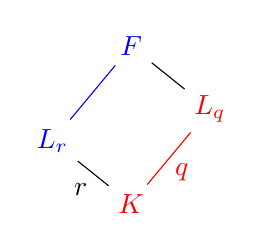
\begin{tikzpicture}

            \node [red] (Q1) at (0,0) {$K$};
            \node [red] (Q2) at (1,1.2) {$L_q$};
            \node [blue] (Q3) at (0,2) {$F$};
            \node [blue] (Q4) at (-1,0.8) {$L_r$};
        
            \draw [red] (Q1)--(Q2) node [pos=0.8, below,inner sep=0.25cm] {$q$};
            \draw (Q1)--(Q4) node [pos=0.9, below,inner sep=0.25cm] {$r$};
            \draw [blue] (Q3)--(Q4);
            \draw (Q2)--(Q3);
        
        \end{tikzpicture}
        \caption[short]{Subfields of a $C_{pq}$-extension}
    \end{figure}

    Again, the result follows immediately from the table and \eqref{eqn_local_contr}.
    
\end{proof}

We are finally ready to prove the main result of this section, from which Theorem \ref{thm_consistent_cyclic} will follow. 

\begin{lemma}\label{lem_Cd_odd}
    Let $d$ be a composite, odd squarefree integer and let $F/K$ be a Galois extension of number fields such that $\Gal(F/K)=C_{d}$. Let $E/\QQ$ be an elliptic curve with semistable reduction at $2$ and $3$ and let $L_k$ be the intermediate fields such that $\Gal(F/L_k)=C_{d/k}$. If 
    $$\Theta_d=\sum_{k\mid d}\mu(k)C_k\in B(C_d),$$
    then $C(\Theta_d)\in\QQss$.
\end{lemma}

\begin{proof}
    Let $n$ be the number of distinct prime numbers dividing $d$, so that $d=p_1\ldots p_n$ for some distinct odd primes $p_i$. We prove this result by induction. The base case for $n=2$ is the content of Lemma \ref{lem_Cpq}. Assume that the result holds for squarefree cyclic Galois extensions with $n-1$ prime factors and consider the two sets of subgroups
    $$\mathcal{A}=\{C_k:p_n\mid k\}\quad\text{and}\quad\mathcal{B}=\{C_k:p_n\nmid k\},$$
    which are clearly a partition of subgroups of $C_d$. Furthermore, the fields $\{F^{C_k}:C_k\in\mathcal{A}\}$ are precisely the intermediate fields of $L_{d/p_n}/K$, while the fields $\{F^{C_k}:C_k\in\mathcal{B}\}$ are the intermediate fields of $F/L_{p_n}$.
    Let 
    $$\Theta_\mathcal{A}=\sum_{H\in\mathcal{A}}\mu(|H|/p_n)H\quad\text{and}\quad\Theta_\mathcal{B}=\sum_{H\in\mathcal{B}}\mu(|H|)H$$
    and we note that
    \begin{equation}\label{eqn_theta}
        \Theta_d=\sum_{k\mid d}\mu(k)C_k=\sum_{p_n\nmid k\mid d}\mu(|C_k|)C_k-\sum_{p_n\mid k\mid d}\mu(|C_k|/p_n)C_k=\Theta_\mathcal{B}-\Theta_\mathcal{A}.
    \end{equation}
    Since $\Gal(L_{d/p_n}/K)=\Gal(F/L_{p_n})=C_{d/p_n}$, it follows from the inductive hypothesis applied to $L_{d/p_n}/K$ and $F/L_{p_n}$ that $C(\Theta_\mathcal{A}),C(\Theta_\mathcal{B})\in\QQss$, and therefore
    $$C(\Theta_d)=\frac{C(\Theta_\mathcal{B})}{C(\Theta_\mathcal{A})}\in\QQss,$$ 
    as desired.
    \begin{figure}[!ht]
        \centering
        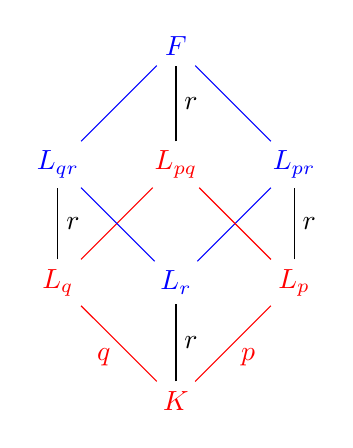
\begin{tikzpicture}

            \node [red] (Q1) at (0,0) {$K$};
            \node [red] (Q2) at (-1.5,1.5) {$L_q$};
            \node [blue] (Q3) at (0,1.5) {$L_r$};
            \node [red] (Q4) at (1.5,1.5) {$L_p$};
            \node [blue] (Q5) at (-1.5,3) {$L_{qr}$};
            \node [red] (Q6) at (0,3) {$L_{pq}$};
            \node [blue] (Q7) at (1.5,3) {$L_{pr}$};
            \node [blue] (Q8) at (0,4.5) {$F$};

            \draw [red] (Q1)--(Q2) node [pos=0.7, below,inner sep=0.25cm] {$q$};
            \draw [red] (Q1)--(Q4) node [pos=0.7, below,inner sep=0.25cm] {$p$};
            \draw (Q1)--(Q3) node [pos=0.5, right,inner sep=0.1cm] {$r$};
            \draw (Q2)--(Q5) node [pos=0.5, right,inner sep=0.1cm] {$r$};
            \draw (Q2)--(Q6) [red];
            \draw (Q3)--(Q5) [blue];
            \draw (Q3)--(Q7) [blue];
            \draw (Q4)--(Q6) [red];
            \draw (Q4)--(Q7) node [pos=0.5, right,inner sep=0.1cm] {$r$};
            \draw (Q5)--(Q8) [blue];
            \draw (Q6)--(Q8) node [pos=0.5, right,inner sep=0.1cm] {$r$};
            \draw (Q7)--(Q8) [blue];
        
        \end{tikzpicture}
        \caption[short]{Partition of $n=3$ into $n=2$. Red fields are in $\mathcal{A}$ while blue fields are in $\mathcal{B}$.}
    \end{figure}
\end{proof}

The proof of Theorem \ref{thm_consistent_cyclic} for odd $d$ is now straightforward.

\begin{proof}[Proof of Theorem \ref{thm_consistent_cyclic} for odd $d$]
    The proof is divided into two cases depending on whether $d$ is the power of a prime or not. Suppose first that $d$ is not, so that $\rad(d)$ is a squarefree \textbf{composite} number. Then $\Theta_d=\sum_{k\mid d}\mu(k)C_k\in B(C_d)$ is the $\psi_d$-relation of a faithful character of $C_d$. The subgroups appearing on $\Theta_d$ are the subgroups of $C_{\rad(d)}$ and therefore by Lemma \ref{lem_Cd_odd} applied to the $C_{\rad(d)}$ extension $F/F^{C_{\rad(d)}}$, it follows that 
    $$C(\Theta_d)\in\QQss,$$ and therefore it is the norm of an element for any quadratic extension of $\QQ$. 

    If $d=q^n$ for some odd prime $q$ and $n\geq1$, then Lemma \ref{lem_relation} shows that $\Theta_d=C_1-C_q$ is the $\psi_d$-relation of a faithful character of $C_d$. Lemma \ref{lem_Cp} applied to the $C_q$ extension $F/F^{C_q}$ proves that 
    $$C(\Theta_d)=\frac{C(C_1)}{C(C_q)}\in N_{\QQ(\sqrt{q^*})/\QQ}(\QQ(\sqrt{q^*})^{\times}).$$ 
    By Lemma \ref{lem_subfields} this is the only quadratic subfield of $\QQ(\zeta_{q^n})$, so the result follows.
\end{proof}

 
\subsection{Even Cyclic Extensions}
More care is required to prove Theorem \ref{thm_consistent_cyclic} for even $d$. This difficulty mainly lies in the case when $d$ is only divisible by one odd prime $q$. Consequently, we break down the proof into three distinct cases according to the number of odd prime divisors of $d$. If $d$ has more than one odd prime divisor, then the result follows without much work from Lemma \ref{lem_Cd_odd}, so we prove this first.

\begin{proof}[Proof of Theorem \ref{thm_consistent_cyclic} for even $d$ with more than one odd prime divisor]
    By Remark \ref{rem_radical}, recall that the subgroups present in $\Theta_d$ are precisely those such that $C_k\leq C_{\rad(d)}$, and so following a similar idea to Lemma \ref{lem_Cd_odd}, we define
    $$\mathcal{A}=\{C_k :2\mid k\mid\rad(d)\}\quad\text{and}\quad\mathcal{B}=\{C_k:2\nmid k\mid\rad(d)\},$$
    together with
    $$\Theta_\mathcal{A}=\sum_{H\in\mathcal{A}}\mu(|H|/2)H\quad\text{and}\quad\Theta_\mathcal{B}=\sum_{H\in\mathcal{B}}\mu(|H|)H. $$ 
    For each $k\mid d$, let $L_k=F^{C_{d/k}}$ be the unique subfield of degree $k$ over $K$. The fields $\{F^{C_k}:C_k\in\mathcal{A}\}$ are the intermediate fields of $L_{d/2}/L_{d/\rad(d)}$ and the fields $\{F^{C_k}:C_k\in\mathcal{A}\}$ are the intermediate fields of $F/L_{2d/\rad(d)}$. However, note that 
    $$\Gal(L_{d/2}/L_{d/\rad(d)})=\Gal(F/L_{2d/\rad(d)})=C_{\rad(d)/2},$$
    and by assumption $\rad(d)/2$ is an odd number with more than one prime factor. Then Lemma \ref{lem_subfields} applied to $L_{d/2}/L_{d/\rad(d)}$ and $F/L_{2d/\rad(d)}$ gives $\Theta_\mathcal{A},\Theta_\mathcal{B}\in\QQss$. The calculation in \eqref{eqn_theta} shows that $\Theta_d=\Theta_\mathcal{B}-\Theta_\mathcal{A}$ and therefore 
    $$C(\Theta_d)=\frac{C(\Theta_\mathcal{B})}{C(\Theta_\mathcal{A})}\in\QQss$$
    is the norm of any quadratic extension.
\end{proof}

If $d$ has no odd primes factors, then $d=2^m$ for some $m\geq1$. With the results we have proven in Sections \ref{sec_type2EC} and \ref{sec_oddcyclic}, the proof of Theorem \ref{thm_consistent_cyclic} for this case is also fairly straightforward.

\begin{proof}[Proof of Theorem \ref{thm_consistent_cyclic} for $d=2^m$]
    If $d=2^m$, then $\Theta_{d}=C_1-C_2$ and therefore if $L=F^{C_2}$, then 
    $$C(\Theta_{d})=\frac{C_{E/F}}{C_{E/L}}.$$
    %Recall from Lemma \ref{lem_subfields}, that the quadratic subfields of $\QQ(\zeta_{2^m})$ depend on $m=1$, $m=2$ or $m\geq3$, so we consider all three cases. 
    If $m=1$, then $\QQ(\zeta_2)=\QQ$ and there is nothing to prove, so assume that $m\geq2$. As usual, we fix a prime $\pp$ of $K$ of bad reduction and we compute $\Cp(\Theta_d)$. Let $\bar\pp$ be a prime in $L$ above $\pp$. If $\bar\pp$ has multiplicative reduction, then we remark that Table \ref{table_Cp} also applies for $q=2$, and therefore $\Cpb(\Theta_d)$ is a rational square up to factors of $2$. Lemma \ref{lem_subfields} shows that the only subfields of $\QQ(\zeta_{2^m})$ are $\QQ(i),\QQ(\sqrt{2})$ and $\QQ(\sqrt{-2})$, and since
    $$2=\Norm_{\QQ(i)}(1+i)=\Norm_{\QQ(\sqrt{-2})}(\sqrt{-2})=\Norm_{\QQ(\sqrt{2})}(2+\sqrt{2}),$$
    it follows that $\Cpb(\Theta_d)$ is a norm from every quadratic subfield of $\QQ(\zeta_{2^m})$.

    Assume now that $\bar\pp$ has additive reduction, let $e_\pp$ and $f_\pp$ be the ramification and inertia degree of $\pp$ over $L$, and note that $e_\pp f_\pp\mid 2^{m-1}$. If $e_\pp f_\pp\neq 2^{m-1}$ then $g_\pp=2^{m-1}/(e_\pp f_\pp)$, the number of primes in $L$ above $\pp$, is even. Since they all have the same local behaviour, it follows that $\Cp(\Theta_d)=\Cpb(\Theta_d)^{g_\pp}\in\QQss$. Hence, we might assume that $e_\pp f_\pp=2^{m-1}$. To compute $\Dp(\Theta_d)$, we note that if $f_\pp\neq 1$, then it is even and hence $N(\bar\pp)=N(\pp)^{f_\pp}\in\QQss$. If $f_\pp=1$, then $e_\pp=2^{m-1}$ and $\pp$ is totally ramified in $L/K$, which is equivalent to being totally ramified in $F/K$. In this case, $\Dp(\Theta_d)$ is a power of $N(\pp)=p^s$ for some rational prime $p$ and $s\geq 1$ and by Proposition \ref{prop_totally_ramified}, it follows that $p^s\equiv 1\pmod{2^m}$. If $s$ is even, then $\Dp(\Theta_d)\in\QQss$ so assume it is odd. If $m=2$, then $p\equiv 1\pmod{4}$ is a norm from $\QQ(i)$ as desired. If $m\geq 3$, then it also follows that $p\equiv 1\pmod{8}$ since $(\ZZ/8\ZZ)^*=C_2\times C_2$. Then
    $$\left(\frac{-1}{p}\right)=\left(\frac{2}{p}\right)=\left(\frac{-2}{p}\right)=1,$$
    so $p$ splits in $\QQ(i),\QQ(\sqrt{2})$ and $\QQ(\sqrt{-2})$. Since they all have class number $1$, $p$ is a norm from all of them, as desired.

    Finally, we compute $\Tp(\Theta_d)$. Since $2$ is a norm of $\QQ(i),\QQ(\sqrt{2})$ and $\QQ(\sqrt{-2})$, we only need to control the contribution of $3$. Under the assumption that $e_\pp f_\pp=2^{m-1}$, $\bar\pp$ is either inert or ramifies in $F/L$, but it can never split. If $n=\nu_{\bar\pp}(\Delta_{E,\bar\pp}^{\min})$, we can see from Lemma \ref{lem_add_tam} that a factor of $3$ can only arise if $E$ has potentially good reduction at $\bar\pp$, $\gcd(n,12)=2$ and $\bar\pp$ ramifies in $L/K$, so assume this is the case. Then let $L'=F^{C_4}$ and $\pp'=\bar\pp\cap L'$, and note that $E$ has additive reduction at $\pp'$. If $e_\pp\geq 2$, then $\pp'$ ramifies in $L/L'$ and the valuation of the minimal discriminant at $\pp'$ is either $n/2$ or $(n+12)/2$. In either case, $\gcd(\nu_{\pp'}(\Delta_{E,\pp'}^{\min}),12)=1$, a contradiction. Hence, $e_\pp=1$ and therefore $\pp'$ is inert in $L/L'$. But then we are precisely under the conditions of Lemma \ref{lem_notthree}, which implies that $\sqrt{B}\not\in F_\fP$, where $\fP$ is the unique prime in $F$ above $\bar\pp$. Hence, $c_\fP(E/F)=1$ and hence $\Tp(\Theta_d)\in\QQss$. We have covered all cases, and the result follows.
\end{proof}

The remaining of this section is therefore devoted to the case when $d$ is divisible by one odd prime $q$, so $d=2^mq^n$. 
%When $d$ has this form, then $\Theta_d=C_1-C_2-C_q+C_{2q}$ and therefore fix $\Theta_d$ to have this expression for the remaining of this section. 
Recall that the quadratic subfields of $\QQ(\zeta_{2^mq^n})$ depend on whether $m=1$, $m=2$ or $m\geq 3$. Consequently, we prove three results that will be essential to prove the general version of each different case. The first covers the case $m=1$.

\begin{lemma}\label{lem_C2p}
    Let $q$ be an odd prime and let $F/K$ be a Galois extension of number fields such that $\Gal(F/K)=C_{2q}$ and let $L_k=F^{C_{2q/k}}$ be the intermediate fields such that $[L_k:K]=k$. Let $E/\QQ$ be an elliptic curve and let $\Theta_{2q}=C_{2q}-C_q-C_2+C_1\in B(C_{2q})$. Then
    $$C(\Theta_{2q})=\frac{C_{E/F}C_{E/K}}{C_{E/L_2}C_{E/L_q}}$$
    is a norm from $\QQ(\sqrt{q^*})$.
\end{lemma}

\begin{proof}
    Similarly to the proofs of Lemma \ref{lem_Cp} and \ref{lem_Cpq}, let $\pp$ be a prime in $K$ and assume that $\Delta_E=\Delta_{E,\pp}^{\min}$. The splitting behaviour of a prime $\pp$ in $K$ is again determined by $e_\pp$ and $f_\pp$ and therefore if $\pp$ has multiplicative reduction $\Dp(\Theta_{2q})=1$ and the following table records $\Tp(\Theta_{2q})$.

    \begin{table}[!ht]
        \centering
        \begin{tabular}{|l|l|l|l|l|l|l|}
        \hline
        $e_\pp$ & $f_\pp$  & $\Tp(C_{2q})$ & $\Tp(C_2)$ & $\Tp(C_q)$ & $\Tp(C_1)$ & $\Tp(\Theta_{2q})$ \\ \hline
        $1$ & $1$ & $n;\tilde{n}$ & $n^q;\tilde{n}^q$ & $n^2;\tilde{n}^2$ & $n^{2q};\tilde{n}^{2q}$ & $\square$ \\ \hline
        $1$ & $q$ & $n;\tilde{n}$ & $n;\tilde{n}$ & $n^2;\tilde{n}^2$ & $n^2;\tilde{n}^2$ & $\square$ \\ \hline
        $1$ & $2$ & $n;\tilde{n}$ & $n^q;\tilde{n}^q$ & $n;n$ & $n^q;n^q$ & $\square$ \\ \hline
        $1$ & $2q$ & $n;\tilde{n}$ & $n;\tilde{n}$ & $n;n$ & $n;n$ & $\square$ \\ \hline
        $q$ & $1$ & $n;\tilde{n}$ & $qn;\tilde{n}$ & $n^2;\tilde{n}^2$ & $q^2n^2;\tilde{n}^2$ & $q\square;\square$ \\ \hline
        $q$ & $2$ & $n;\tilde{n}$ & $qn;\tilde{n}$ & $n;n$ & $qn;n$ & $\square$ \\ \hline
        $2$ & $1$ & $n;\tilde{n}$ & $n^q;\tilde{n}^q$ & $2n;1$ & $2^qn^q;1^q$ & $\square$ \\ \hline
        $2$ & $q$ & $n;\tilde{n}$ & $n;\tilde{n}$ & $2n;1$ & $2n;1$ & $\square$ \\ \hline
        $2q$ & $1$ & $n;\tilde{n}$ & $qn;\tilde{n}$ & $2n;1$ & $2qn;1$ & $\square$ \\ \hline
        \end{tabular}
        \caption{Contribution of multiplicative reduction primes in a $C_{2q}$ extension.}
    \end{table}

    Since $q$ is a norm from $\QQ(\sqrt{q^*})$, then $\Tp(\Theta_{2q})$ is also a norm. Now assume that $\pp$ has additive reduction and let $p\ZZ=\pp\cap\QQ$. We first consider the contribution of the Tamagawa numbers. Note that $L_q/K$ and $F/L_2$ are $C_q$ extensions and therefore $\Tp(\Theta_{2q})\in\QQss$ if $q\neq 3$ and a square up to factors of $3$ if $q=3$. In either case, $\Tp(\Theta_{2q})$ is a norm from $\QQ(\sqrt{q^*})$.

    Finally, to compute $\Dp(\Theta_{2q})$, let $n=\nu_\pp(\Delta_{E,\pp}^{\min})$ and note that all terms cancel unless $\pp$ ramifies in $F$. If $e_\pp=2$, then
    \begin{equation}\label{eqn_ep=2}
        \Dp(C_{2q})=\Dp(C_2)=1,\quad \Dp(C_q)=N(\pp)^{\floor{\frac{2n}{12}}}\quad\text{and}\quad \Dp(C_1)=N(\pp)^{q\floor{\frac{2n}{12}}},
    \end{equation}
    and therefore $D(\Theta_{2q})=N(\pp)^{(q-1)\floor{n/6}}\in\QQss$, a rational square. If $q\mid e_\pp$, then $q\mid N(\pp)-1$ by Proposition \ref{prop_totally_ramified}, and the reasoning is now identical to Lemma \ref{lem_Cp}. Write $N(\pp)=p^s$ for some $s\geq1$ and note that $\Dp(\Theta_{2q})\in\QQss$ if $s$ is even. Hence, we assume that $s$ is odd. In this case, $p=q$ if $(L_q)_\fP/K_\pp$ is wildly ramified and $p$ splits in $\QQ(q^*)$ if $(L_q)_\fP/K_\pp$ is tamely ramified. In either case, by Corollaries \ref{p-norm} and \ref{cor_psplit_pnorm}, $p$ is a norm from $\QQ(\sqrt{q^*})$, and hence so is $\Dp(\Theta_{2q})$.
    The result follows again from \eqref{eqn_local_contr}.
\end{proof}

Following this, we state and prove the analogous result for $m=2$.

\begin{lemma}\label{lem_C4p}
    Let $q$ be an odd prime and let $F/K$ be a Galois extension of number fields such that $\Gal(F/K)=C_{4q}$ and let $L_k=F^{C_{4q/k}}$ be the intermediate fields such that $[L_k:K]=k$. Let $E/\QQ$ be an elliptic curve with semistable reduction at $2$ and $3$ and let $\Theta_{4q}=C_1-C_2-C_q+C_{2q}$. Then 
    $$C(\Theta_{4q})=\frac{C_{E/F}C_{E/L_2}}{C_{E/L_4}C_{E/L_{2q}}}$$
    is a norm from $\QQ(i),\QQ(\sqrt{q})$ and $\QQ(\sqrt{-q})$. Moreover, $\Tp(\Theta_{4q})\in\QQss$ for any prime $\pp$ in $K$, and $\Dp(\Theta_{4q})\in\QQss$ unless $E$ has additive reduction at $\pp$ and $\pp$ is totally ramified in $F/K$.
\end{lemma}

\begin{proof}
    All fields appearing in the product are intermediate fields of $F/L_2$, and $\Gal(F/L_2)=C_{2q}$. Let $\pp$ be a prime in $K$, let $\bar\pp\mid\pp$ be a prime above $\pp$ in $L_2$ and let $p\ZZ=\pp\cap\QQ$. Assume also that $\Delta_E=\Delta_{E,\pp}^{\min}$. Lemma \ref{lem_C2p} shows that if $E$ has multiplicative reduction over $\bar\pp$, $C_{\fP\mid\bar\pp}(\Theta_{4q})\in\QQss$ unless $e_{\bar\pp}=q$ and $f_{\bar\pp}=1$ over $F$. When this holds, $\bar\pp$ ramifies in $L_{2q}/L_2$ and is split in $L_4/L_2$, and this forces $\pp$ to split in $L_2/K$ too. Hence, $\pp=\bar\pp\bar\pp'$ for two \textbf{distinct} primes in $K$ that have the same local behaviour and therefore $\Cp(\Theta_{4q})=C_{\fP\mid\bar\pp}(\Theta_{4q})C_{\fP\mid\bar\pp'}(\Theta_{4q})=C_{\fP\mid\bar\pp}(\Theta_{4q})^2\in\QQss$, as desired.

    \begin{figure}[!ht]
        \centering
        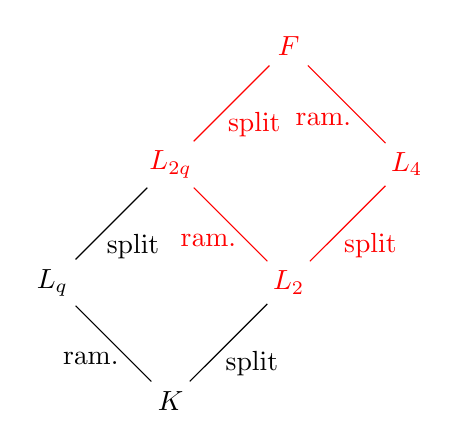
\begin{tikzpicture}

            \node (Q1) at (0,0) {$K$};
            \node (Q2) at (-1.5,1.5) {$L_q$};
            \node [red] (Q3) at (3,3) {$L_4$};
            \node [red] (Q4) at (1.5,1.5) {$L_2$};
            \node [red] (Q5) at (1.5,4.5) {$F$};
            \node [red] (Q6) at (0,3) {$L_{2q}$};
            

            \draw (Q1)--(Q2) node [pos=0.8, below,inner sep=0.4cm] {ram.};
            \draw (Q1)--(Q4) node [pos=0.8, below,inner sep=0.4cm] {split};
            \draw (Q2)--(Q6) node [pos=0.8, below,inner sep=0.4cm] {split};
            \draw [red] (Q3)--(Q5) node [pos=0.8, below,inner sep=0.4cm] {ram.};
            \draw [red] (Q4)--(Q6) node [pos=0.8, below,inner sep=0.4cm] {ram.};
            \draw [red] (Q6)--(Q5) node [pos=0.8, below,inner sep=0.4cm] {split};
            \draw [red] (Q4)--(Q3) node [pos=0.8, below,inner sep=0.4cm] {split};
        \end{tikzpicture}
        \caption[short]{\centering Field diagram for a $C_{4q}$ extension, together with the splitting\newline behaviour of a prime $\pp$ in $L_2$ with $e_\pp=q$ and $f_\pp=1$ over $F$.}
    \end{figure}

    Assume now that $E$ has additive reduction over $\bar\pp$. When $q=3$, controlling the Tamagawa numbers is lengthy, so we leave it for the end. We calculate first $\Dp(\Theta_{4q})$, which is $1$ unless $\bar\pp$ ramifies in $L/F_2$ (equivalently, $\pp$ ramifies in $L/K$). If $\pp$ is inert in $L_2/K$, then $N(\bar{\pp})\in\QQss$ and hence the size of all residues fields above $\pp$ are also squares and consequently $\Dp(\Theta_{4q})\in\QQss$ using Lemma \ref{lem_Dterms}. If $\pp=\bar\pp\bar\pp'$ splits, then $D_{\fP\mid\bar\fp}(\Theta_{4q})=D_{\fP\mid\bar\fp'}(\Theta_{4q})$, and therefore $\Dp(\Theta_{4_q})\in\QQss$ too. Finally, assume that $\pp=\bar\pp^2$ ramifies in $L_2/K$, which implies that $\bar\fp$ also ramifies in $L_4/L_2$. On the other hand, if $\bar\pp$ is unramified at $L_{2q}/L_2$, \eqref{eqn_ep=2} during the proof of Lemma \ref{lem_C2p} shows that $\Dp(\Theta_{4q})\in\QQss$ too. 

    We are therefore left with the case where $\pp$ is totally ramified in $F/K$, and Proposition \ref{prop_totally_ramified} implies that $4q\mid N(\pp)-1$. If we let $n=\nu_{\pp}(\Delta_{E,\pp}^{\min})$, Lemma \ref{lem_Dterms} implies that 
    \begin{equation*}\label{eqn_DtermsC4p}
        \Dp(\Theta_{4q})=N(\pp)^{\floor{\frac{n}{6}}-\floor{\frac{n}{3}}-\floor{\frac{qn}{6}}+\floor{\frac{qn}{3}}}.
    \end{equation*}
    Again, the parity of the expression only depends on $q,n\pmod{12}$. One can easily check that for $n\in\{2,3,4,6,8,9,10\}$ and $q\in\{1,5,7,11\}$, the above expression is a square unless $q\equiv 3\pmod{4}$ and $n$ is odd, so we assume this is the case. Write $N(\pp)=p^s$ for some $s\geq1$, which satisfies $p^s\equiv1\pmod{4q}$. If $s$ is even, then $\Dp(\Theta_{4q})\in\QQss$, so assume that $s$ is odd. Since $p^s\equiv1\pmod{4}$, this implies that $p\equiv1\pmod{4}$ and hence $p$ is a norm from $\QQ(i)$, which implies that $\Dp(\Theta_{4q})$ is a norm from $\QQ(i)$ too. Furthermore, the fact that $p^s\equiv1\pmod{4q}$ implies that
    $$\left(\frac{-q}{p}\right)=\left(\frac{q}{p}\right)=\left(\frac{p}{q}\right)=\left(\frac{p^s}{q}\right)=1,$$
    and therefore $p$ splits both in $\QQ(\sqrt{q})$ and $\QQ(\sqrt{-q})$. Since $q\equiv3\pmod{4}$, both fields have odd class number (Theorem \ref{thm_class_number}), and hence $p$ and $\Dp(\Theta_{4q})$ are norms from $\QQ(\sqrt{q})$ and $\QQ(\sqrt{-q})$ as desired. 

    Finally, we discuss Tamagawa numbers. Note that $L_{2q}/L_2$ and $F/L_4$ are $C_q$ extensions and therefore by Lemma \ref{lem_Cp} it follows that $\Dp(\Theta_{4q})\in\QQss$ if $q\neq3$. If $q=3$, it is also the case that $\Dp(\Theta_{4q})\in\QQss$, but more work is required. We prove this as a separate lemma, from which the result follows.    
\end{proof}

\begin{lemma}
    Let $L/K$ be a Galois extension of number fields with $\Gal(L/K)=C_{12}$ and let $L_k=F^{C_{12/k}}$ be the intermediate fields such that $[L_k:K]=k$. Let $E/\QQ$ be an elliptic curve and let $\pp$ be a prime in $K$ not dividing $2$ or $3$ such that $E$ has potentially good reduction at $\pp$. If $\Theta_{12}=C_1-C_2-C_3+C_6\in B(C_{12})$, then $$\Tp(\Theta_{12})=\frac{\Tp(E/F)\Tp(E/L_2)}{\Tp(E/L_6)\Tp(E/L_4)}\in\QQss.$$
\end{lemma}
\begin{proof}
    Let $\bar\pp$ be a prime in $L_2$ above $\pp$ and let $n=\nu_{\bar\pp}(\Delta_{E,\bar\pp}^{\min})$ be the minimal discriminant of $E$ at $\bar\pp$. If $\pp$ is unramified in $L_3/K$, then so is $\bar\pp$ in $L_6/L_2$ and the primes above them in $F/L_4$. From Lemma \ref{lem_Cp}, we know that that the product of Tamagawa numbers in unramified $C_3$ extensions is a square, so assume that $\pp$ ramifies in $L_3/K$.

    The proof is now divided in three cases, depending on the splitting behaviour of $\pp$ in $L_2$. If $\pp$ splits in $L_2/K$, then $\pp=\bar\pp\bar\pp'$ where $\bar\pp$ and $\bar\pp'$ have the same local behaviour. Therefore, $T_{\fP\mid\pp}(\Theta_{12})=T_{\fP\mid\bar\pp}(\Theta_{12})T_{\fP\mid\bar\pp'}(\Theta_{12})\in\QQss$. 
    
    Next, suppose that $\pp$ is inert in $L_2/K$, which implies that $\bar\pp$ is either inert or ramified in $L_4/L_2$. Let $\fP$ be the prime in $L_4$ above $\bar\pp$. If $\bar\pp$ is inert in $L_4/L_2$, then the valuation of the minimal discriminant of $E$ at $\fP$ is also $n$ and the splitting behaviour of $\bar\pp$ in $L_6/L_2$ coincides with the splitting behaviour of $\fP$ in $F/L_4$. Hence, 
    $$\frac{\Tp(E/F)}{\Tp(E/L_4)}=\frac{\Tp(E/L_6)}{\Tp(E/L_2)},$$
    and therefore $\Tp(\Theta_{12})=1$. The case where $\bar\pp$ is ramified in $L_4/L_2$ is more subtle. We have already seen that in ramified $C_3$ extensions we cannot obtain factors of $2$. Upon inspection of Lemma \ref{lem_add_tam}, one can easily show that the Tamagawa numbers cancel out if $\gcd(n,12)\in\{3,4,6,12\}$, so we only need to consider the case $\gcd(n,12)=2$. Since $\Gal((L_4)_\fP/K_\pp)=C_4$ and $e_{\fP\mid\pp}=f_{\fP\mid\pp}=2$, Lemma \ref{lem_notthree} shows that $\sqrt{B}\not\in F_{\fP}$ and therefore $c_\fP(E/F)=1$, which implies that $\Dp(\Theta_{12})\in\QQss$.

    Finally, assume that $\pp$ ramifies in $L_2/K$ so that $\pp=\bar\pp^2$. This immediately implies that $\bar\pp$ also ramifies in $L_4/L_2$, and therefore $\pp$ is totally ramified in $F/K$. As mentioned above, the Tamagawa numbers cancel unless $\gcd(n,12)=2$. However, recall that $E$ has potentially good reduction at $\pp$, and since $\pp=\bar\pp^2$ ramifies, then the valuation of the minimal discriminant at $\pp$ is $n/2$ or $(n+12)/2$. But then $\gcd(\nu_\pp(\Delta_{E,\pp}^{\min}),12)=\gcd(n/2,12)=1$, a contradiction. Hence, $\Tp(\Theta_{12})\in\QQss$ as desired.
\end{proof}

Finally, we state and prove the last result, from which the case $m\geq3$ follows easily. One needs to check that the product of local factors is the norm of many quadratic subfields; thankfully, Lemma \ref{lem_C4p} has done most of work required.

\begin{lemma}\label{lem_C8p}
    Let $q$ be an odd prime and let $F/K$ be a Galois extension of number fields such that $\Gal(F/K)=C_{8q}$ and let $L_k=F^{C_{8q/k}}$ be the intermediate fields such that $[L_k:K]=k$. Let $E/\QQ$ be an elliptic curve with semistable reduction at $2$ and $3$ and let $\Theta_{8q}=C_1-C_2-C_q+C_{2q}$. Then 
    $$C(\Theta_{8q})=\frac{C_{E/F}C_{E/L_4}}{C_{E/L_8}C_{E/L_{4q}}}\in\QQss.$$
    %is a norm from $\QQ(\sqrt{D})$ for each $D\in\{-1,\pm2,\pm q,\pm 2q\}$.
\end{lemma}

\begin{proof}
    We prove the result locally for all primes in $L_2$, and note $\Gal(F/L_2)=4q$. Let $\bar\pp$ and assume that $\Delta_E=\Delta_{E,\bar\pp}^{\min}$. Since the relation $\Theta_{4q}=C_1-C_2-C_q+C_{2q}\in B(C_{4q})$ has the same fixed fields as $\Theta_{8q}$, by Lemma \ref{lem_C4p}, we know that $\Tpb(\Theta_{8q})\in\QQss$ for any $\bar\pp$ and $\Dpb(\Theta_{8q})\in\QQss$ too unless $\bar\pp$ is totally ramified in $F/L_2$ and $E$ has potentially good reduction at $\bar\pp$, so assume this is the case. If $\pp=\bar\pp\cap K$, then it also follows that $\pp$ is totally ramified in $F/K$ and $E$ has potentially good reduction at $\pp$. If $n=\nu_{\bar\pp}(\Delta_{E,\bar\pp}^{\min})$, then recall from Lemma \ref{lem_C4p} that 
    $$\Dpb(\Theta_{8q})=N(\bar\pp)^{\floor{\frac{n}{6}}-\floor{\frac{n}{3}}-\floor{\frac{qn}{6}}+\floor{\frac{qn}{3}}},$$
    and that the exponent is even unless $n$ is odd and $q\equiv 3\pmod{4}$. However, $\pp=\bar\pp^2$ is ramified in $L_2/K$ and therefore $n\equiv 2\nu_\pp(\Delta_{E,\pp}^{\min})\pmod{12}$. That is, $n$ is even and therefore $\Dpb(\Theta_{8q})\in\QQss$ as desired.
\end{proof}
%%% THIS IS ALL PROBABLY NOT NEEDED NOW
%Again, $\Dp(\Theta_{8q})$ does not change up to squares if $\Delta_{E}$ is rescaled so assume that $\Delta_{E}=\Delta_{E,\pp}^{\min}$. Under these assumptions, $\Dpb(\Theta_{8q})=\Dp(\Theta_{8q})$ is a power of $N(\pp)=N(\bar\pp)=p^s$ for some rational prime $p$ and $s\geq1$. If $s$ is even, then $\Dpb(\Theta_{8q})\in\QQss$, so assume that $s$ is odd. In addition, by Proposition \ref{prop_totally_ramified}, it follows that $p^s\equiv 1\pmod{8q}$. Since $s$ is odd and $(\ZZ/8\ZZ)^*=C_2\times C_2$, it follows that $p\equiv 1\pmod{8}$ and therefore
%\begin{equation}\label{eqn_psplitsin2}
%    \left(\frac{-1}{p}\right)=\left(\frac{2}{p}\right)=\left(\frac{-2}{p}\right)=1.
%\end{equation}
%Furthermore, since $p^s\equiv1\pmod{8s}$ and $s$ is odd, then 
%\begin{equation}\label{eqn_psplitsinq}
%    \left(\frac{-q}{p}\right)=\left(\frac{q}{p}\right)=\left(\frac{p}{q}\right)=1.
%\end{equation}
%Combining \eqref{eqn_psplitsin2} and \eqref{eqn_psplitsinq} together with multiplicity of the Legendre symbol, it follows that $p$ splits in every quadratic subfield $\QQ(\sqrt{D})$ for $D\in\{-1,\pm2,\pm q,\pm2q\}$.


We are now ready to prove the remaining case of Theorem \ref{thm_consistent_cyclic}.

\begin{proof}[Proof of Theorem \ref{thm_consistent_cyclic} for $d$ even and with one odd prime factor.]
    In this case, write $d=2^mq^n$ for $n,m\geq 1$ and note that $\Theta_{d}=C_1-C_2-C_q+C_{2q}$ is the $\psi_d$-relation of a faithful character of $C_d$. If $m=1$, Lemma \ref{lem_C2p} applied to the $C_{2q}$ extension $F/F^{C_{2q}}$ shows that $C(\Theta_d)$ is a norm from $\QQ(\sqrt{q^*})$, which is the only subfield of $\QQ(\zeta_{2q^n})$ by Lemma \ref{lem_subfields}. If $m=2$, then Lemma \ref{lem_C4p} applied to the $C_{4q}$ extension $F/F^{C_{4q}}$ shows that $C(\Theta_{d})$ is a norm from $\QQ(i),\QQ(\sqrt{q})$ and $\QQ(\sqrt{-q})$, which are all quadratic subfields of $\QQ(\zeta_{4q^n})$. Finally, if $m\geq3$, Lemma \ref{lem_C8p} applied to $F/F^{C_{8q}}$ shows that $C(\Theta_{8q})\in\QQss$, which is the norm from any quadratic subfield. The result follows.
\end{proof}



\newpage
\section{Odd Extensions and Consistency with BSD}\label{sec_odd}
%\subsection{Norm Relations in Odd Order Extensions}

In this section we prove the analogous result to the previous section when $F / \bQ$ is any Galois extension of odd order. As discussed in \S\ref{sec-norm-rels-test}, we expect our Norms Relations test to be "uninteresting"  because root number computations don't predict positive rank.  

\begin{thm}\label{odd-exts}
 Let $E / \bQ$ be an elliptic curve, $F / \bQ$ be an extension of odd order with Galois group $G$. 
 
Assume that $E$ has good or multiplicative reduction at $2$ and $3$. 
Take any representation $\rho$ of $G$ with quadratic subfield $\bQ(\sqrt{D}) \subset \bQ(\rho)$ and relation
\begin{equation*}\label{odd-exp} \repnorm{\rho}^{\oplus m} =
 \left(\bigoplus_{\mathfrak{g}\in\Gal(\QQ(\rho)/\QQ)}\rho^{\mathfrak{g}}\right)^{\oplus m }=\bigoplus_i\Ind_{F_i/\QQ}\mathds{1}\ominus\bigoplus_j\Ind_{F'_j/\QQ}\mathds{1}
\end{equation*}
 as in Theorem \ref{thm_positive_rank}. Then
 \[ \frac{\prod_i C_{E/F_i}}{\prod_j C_{E/F_j'}}  \in 
    \begin{cases}
        N_{\bQ(\sqrt{D}) / \bQ}(\bQ(\sqrt{D})^{\times}) & m \ \text{odd}, \\
        (\bQ^{\times})^2 & m \ \text{even}.
    \end{cases} \] 
    In other words, one cannot use Theorem \ref{thm_positive_rank} to conclude that $E / F$ must have positive rank. 
\end{thm}

As in Remark \ref{rephrase-thm}, replacing $\rho$ by the sum of its conjugates by elements of $ \Gal(\bQ(\rho) / \bQ(\sqrt{D}))$, we may assume that $\bQ(\rho) = \bQ(\sqrt{D})$. We take $D \in \bZ \backslash \{0,1 \}$ to be squarefree.

The product of terms we are computing is $C(\Theta)$, where $C \colon \B(G) \to \bQ^{\times}$ is given by $C \colon H \mapsto C_{E / F^H}$, and $\Theta$ is any $\rho$-relation.
We break up the function $C$ into $C = \prod_p C_{\fP \mid p} = \prod_p T_{\fP \mid p} \cdot D_{\fP \mid p}$, ranging over primes $p \in \bQ$,
as defined in Notation \ref{not_contr_fns}.
In Remark \ref{Rem-C-D-loc} we showed that
\begin{equation*}%\label{Dp-loc}
C_{\fP \mid p} = (D_p, C_v)
\end{equation*}
where $C_v$ is a function on $\B(D_p)$ sending $H \mapsto C_v(E / F_w^H)$, for $D_p = \Gal(F_w / \bQ_p)$. The following result will allow us to apply some results from $\S$\ref{sec-norm-rels}.

\begin{thm}\label{odd-c-brauer}
    When $D_p$ has odd order, $C_v(\Psi) \in (\bQ^{\times})^2$ for any Brauer relation $\Psi \in \B(D_p)$. 
\end{thm}

\begin{proof}
    This follows from \cite[Theorem 2.47]{reg-const} and \cite[Theorem 3.2  (Tam)]{reg-const}.
\end{proof}

\begin{cor}
It is enough to prove Theorem \ref{odd-exts} when $m$ is the order of $\repnorm{\rho}$ in $\C(G)$. Thus we need to prove that, given any $
\Theta \in \B(G)$ such that $\bC[\Theta] \simeq \repnorm{\rho}^{\oplus m}$, $\Theta$ is a norm relation for the function $C$. 
\end{cor}

\begin{proof}
    Since $\bQ(\rho)$ is quadratic, we have that rational squares are norms from $\bQ(\rho)$. As $G$ is odd, any choice of $D_p$ is odd. It follows from Theorem \ref{odd-c-brauer} that $C(\Psi) \in (\bQ^{\times})^2$ for all Brauer relations $\Psi \in \B(G)$. Therefore by Proposition \ref{min-to-all}, it is enough to prove Theorem \ref{odd-exts} when $m$ is the order of $\repnorm{\rho}$ in $\C(G)$. Then $m$ divides $|G|$, hence is odd.
\end{proof}

Let $\tau$ be the generator of $\Gal(\bQ(\sqrt{D}) / \bQ)$.
Let $\ff$ be the smallest integer such that $\bQ(\sqrt{D}) \subset \bQ(\zeta_{\ff})$. Then $\ff \mid |G|$, hence is odd. By Remark \ref{conductor}, $\ff = |D|$ and $D \equiv 1 \pmod 4$. The following shows that it is only of interest to consider decomposition groups of exponent divisible by $\ff$.

\begin{cor}\label{rational-res-2}
    Let the exponent of $D_p$ be $b$. If $\ff \nmid b$, then $C_{\fP \mid p}(\Theta) \in (\bQ^{\times})^2$.
\end{cor}

\begin{proof}
    One has $\bQ(\rho) \subset \bQ(\zeta_b) \implies \ff \mid b$ by minimality of $\ff$. Since $\ff \nmid b$, we have $\bQ(\rho) \not\subset \bQ(\zeta_b)$, so $\bQ(\Res_{D_p} \rho) = \bQ$. The corollary then follows from Proposition \ref{rational-res} and Theorem \ref{odd-c-brauer}, noting that since $\C(D_p)$ is odd, multiplication by $2$ is injective. 
\end{proof}

Fix $\Theta = \sum_i n_i H_i \in \B(G)$ with $\bC[\Theta] \simeq \repnorm{\rho}^{\oplus m}$. We prove that at each prime $p$, $C_{\fP \mid p}(\Theta)$ is the norm of an element of $\bQ(\rho)$.  As observed, this depends on $D_p$ and $I_p$. As we deal with each local factor individually, we argue that one can take $D_p = I_p$.

\begin{lemma}\label{tam-up-to-square}
    Let $E / K$ be an elliptic curve. Let $K' / K$ be an extension of number fields odd degree, unramified at the place $v$ of $K$. Then $C_w(E / K') \equiv C_v(E / K) \mod (\bQ^{\times})^2$ for any place $w$ of $K'$ with $ w \mid v$. 
\end{lemma}

\begin{proof}
This is automatic for good reduction and split multiplicative reduction. It is also clear for non-split multiplicative reduction since the residue degree cannot be even (so the reduction type remains non-split at $w$). For additive reduction, see \cite[Lemma 3.12]{reg-const}.
\end{proof}

\begin{lemma}\label{DeqI}
    At a prime $p$, we may assume that $D_p = I_p$ when computing $C_{\fP \mid p}(\Theta)$. 
\end{lemma}

\begin{proof}
Let $p$ have residue degree $f_p$. Let $L / \bQ$ be a Galois extension of degree $f_p$ with cyclic Galois group, such that $p$ is inert in $L$. Further ensure that $F \cap L = \bQ$. Then $\Gal(FL / L) = G' \simeq G$. Let $F_i = F^{H_i}$ and $L_i = F_i L$.

Let $v$ be a place over $p$ in $F_i$. The extension $L_i / F_i$ is Galois, so $v$ is either split or inert in $L_i$.
We claim that $C_v(E / F_i) \equiv \prod_{w | v} C_w(E / L_i) \mod (\bQ^{\times})^2$. Indeed, the number of terms in the product on the right is odd, and by Lemma \ref{tam-up-to-square} $C_v(E / F_i) \equiv C_w(E / L_i) \mod (\bQ^{\times})^2$. 
Letting $C_{\fP \mid \fp}$ be the function on $\B(G')$ defined as in Notation \ref{not_contr_fns} but now $G' = \Gal(FL / L)$, we see that $C_{\fP \mid \fp}(\Theta) \equiv C_{\fP \mid p}(\Theta) \mod (\bQ^{\times})^2$. 
Thus it is equivalent to do our computation in $FL / L$, but here $p$ has residue degree $1$.
\end{proof}

To prove Theorem \ref{odd-exts}, we proceed by computing $C_{\fP \mid p}(\Theta)$ for each reduction type.

\subsubsection*{Good reduction}
If $E / \bQ$ has good reduction at $p$, then by Proposition \ref{prop_local_fns}(i), $C_{\fP \mid p} = 1$.

\subsubsection*{Multiplicative reduction}

\begin{lemma}
Let $E / \bQ_p$ have non-split multiplicative reduction. Then $C_{\fP \mid p}(\Theta) \in (\bQ^{\times})^2$.
\end{lemma}

\begin{proof}
Since $D_p = I_p$, all primes above $p$ have residue degree $1$. Moreover, the ramification degrees are always odd. Thus by Proposition \ref{prop_local_fns}(iii), $C_{\fP \mid p}  = (D_p, \alpha)$
where $\alpha$ is the constant function on $\B(D_p)$ with $\alpha \in \{1, 2\}$, depending on $v_p(\Delta)$ being even or odd. By Proposition \ref{const-fns}, it follows that $C_{\fP \mid p}(\Theta) \in (\bQ^{\times})^2$.
\end{proof}

Now suppose $E / \bQ_p$ has split multiplicative reduction. The reduction type remains split at all places above $p$ within sub-extensions of $F / \bQ$. Let $v_p(\Delta) = n$. Then by Proposition \ref{prop_local_fns}(ii), 
\[ C_{\fP \mid p} = (D_p, D_p, en). \]
Since the $n$ factor is constant, $(D_p, D_p, en)(\Theta) \equiv (D_p, D_p, e)(\Theta) \mod (\bQ^{\times}) ^2$ by Proposition \ref{const-fns} .

We have $D_p = I_p = P_p \ltimes C_l$, where $P_p \triangleleft I_p$ is wild inertia, and $C_l = I_p / P_p$ is the tame quotient. $C_l$ is a cyclic group, with $l \mid p^f - 1 = p - 1$. By Corollary \ref{rational-res-2}, we may consider such $D_p$ with exponent  $p^u l$ for some $u \geq 0$ such that $\ff \mid p^u l$. To compute $C_{\fP \mid p}(\Theta)$, we reduce to the tame quotient.

\begin{lemma}
Let $g \colon \B(C_l) \to \bQ^{\times}$ be defined by $H \mapsto [C_l \colon H] = \dim \bC[C_l / H]$. Let $\Psi = P_p \cdot \Res_{D_p} \Theta / P_p \in \B(C_l)$ Then $(D_p, D_p, e)(\Theta)$ and $g(\Psi)$ differ by a (possible) factor of $p$. 
\end{lemma}

\begin{proof}
%Now, $(D_p, D_p, e)(\Theta)$ is the product of ramification indices at primes above $p$. We separate the $p$-part and tame part of this expression.
Recall that the ramification index of a place $w$ above $p$ corresponding to the double coset $H_i x D_p$ has ramification degree $e_w = \frac{|I_p|}{|H_i \cap I_p^x|} =\frac{|I_p|}{|I_p \cap H^{x^{-1}}|}$.
This is the dimension of the permutation representation $\bC[D_p / D_p \cap H^{x^{-1}}]$.
Let  $D_p \cap H^{x^{-1}} = P' \ltimes C_a$ where $P' \leq P$ and $a | l$. Then the ramification index is $\frac{|P|}{|P'|}\cdot \frac{l}{a}$. 
Taking fixed points under wild inertia, one has the following isomorphism of $D_p$-representations  $$\bC[D_p / D_p \cap H^{x^{-1}}]^{P_p} \simeq \bC[D_p / P_p (D_p \cap H^{x^{-1}})] \simeq \bC[D_p / P_p \ltimes C_a].$$ This permutation representation has dimension $\frac{l}{a}$, so we've killed off the $p$-part. 
Then $$\bC[\Res_{D_p} \Theta]^{P_p} \simeq \left(\Res_{D_p} \rho^{\oplus m} \oplus \tau\left(\Res_{D_p}\rho^{\oplus m}\right)\right)^{P_p},$$
and we can consider these as representations of $D_p / P_p = C_l$.
It follows that $(D_p, D_p, e)(\Theta)$ differs from $g(\Psi)$ up to a (possible) factor of $p$. 
\end{proof}

Now we show that this factor of $p$ is a norm from $\fieldnorm{\rho}$.
Note that if $p = 2$ then $P_p = 1$ since $|P_p| \mid |G|$ which is odd. So we only need to consider this factor of $p$ for $p$ odd.

\begin{lemma}\label{p-norm-odd}
    Let $K = \bQ(\sqrt{D})$, with $\ff$ the smallest positive integer such that $K \subset \bQ(\zeta_{\ff})$. Suppose that $\ff$ is odd. Let $\ff \mid p^u l $, for some odd prime $p$, $u \geq 0$ and $l$ such that $p \equiv 1 \pmod l$. Then $p$ is the norm of an element from $K^{\times}$.
\end{lemma}

\begin{proof}
    Since $\ff$ is odd, one has $D = \prod_{q | \ff} q^*$, the product being taken over primes dividing $\ff$. Note that if $q \not= p$, then since $q \mid l$, we have $p \equiv 1 \pmod l \implies p \equiv 1 \pmod q$. By Corollary \ref{p-one-mod-disc},  $p$ is the norm of a principal fractional ideal of $K$, and by Theorem \ref{p-norm-elem-1} or Theorem \ref{p-norm-elem-2}, it is the norm of an element of $K$.
    %We show that $p$ has residue degree $1$ in the extended genus field $E^{+} = K(\{\sqrt{q^*} \colon q | \ff \})$ of $K$ ({\color{red} cf. appendix}).
    %If $q \not= p$ then $q \mid l$, so $p \equiv 1 \pmod l$. Therefore $p$ splits in any quadratic subfield of $E^{+}$ of discriminant not divisible by $p$. Else, $p$ ramifies in any quadratic subfield with discriminant divisible by $p$. Thus it is clear that $p$ has residue degree $1$ in $E^{+}$, hence also in the genus field $E$, and it follows from theorem \ref{p-principal} that $p$ is the norm of a principal ideal.  Else, we invoke theorem \ref{minus-one-norm}.
\end{proof}

\begin{cor}
Let $E / \bQ_p$ have split multiplicative reduction. Then $C_{\fP \mid p}(\Theta) \in \fieldnorm{\rho}$.
\end{cor}

\begin{proof}
By the previous two results, it is sufficient to show that $g(\Psi) \in \fieldnorm{\rho}$. Let $\phi = (\Res_{D_p} \rho)^{P_p}$, viewed as a representation on $D_p / P_p = C_l$. Then $\Psi$ is a $\phi$-relation. If $\ff \nmid l$ then $\bQ(\phi) = \bQ$. Therefore $\bC[C_l / \Psi] \simeq \phi^{\oplus 2}$, implying that $\Psi = 2\Psi'$ for some $\Psi' \in \B(C_l)$ with $\bC[C_l / \Psi'] = \phi$. Then $g(\Psi) = g(\Psi')^2 \in \fieldnorm{\rho}$. Otherwise, suppose that $\bQ(\phi) = \bQ(\rho)$. It follows from Proposition \ref{index-fn-trivial} that $g(\Psi) \in \fieldnorm{\rho}$.
\end{proof}

\subsubsection*{Additive reduction}

Now suppose that $E / \bQ_p$ has additive reduction. In this case, assume that $p \geq 5$
Write $D_p = \Gal(F_w / \bQ_p)$ for $w \mid p$ a place of $F$.

Again we have $D_p = P_p \ltimes C_l$ with $ l \mid p - 1$, and may assume that $\ff \mid p^u l$ where $p^u l $ is the exponent of $D_p$ by Corollary \ref{rational-res-2}. Let $n = v_p(\Delta_E)$. 

We will compute $D_{\fP \mid p}(\Theta)$ and $T_{\fP \mid p}(\Theta)$ separately. 
By Proposition \ref{prop_local_fns}(iv), (v)
\[ D_{\fP \mid p} = 
    \begin{cases}
        (D_p, D_p,\ p^{\floor{e_ /2}}) & \text{if } E / \bQ_p \text{ has potentially multiplicative reduction}, \\
        (D_p, D_p,\ p^{\floor{en /12}}) & \text{if } E / \bQ_p \text { has potentially good reduction}.
    \end{cases}
    \]
In either case, $D_{\fP \mid p}(\Theta) \in N_{\bQ(\rho) / \bQ}(\bQ(\rho)^{\times})$. Indeed, this takes values $1$ or $p$ in $\bQ^{\times} / (\bQ^{\times})^2$. But $p$ is a norm from $\bQ(\rho)$ by Lemma \ref{p-norm-odd}.

%\[ \left|\frac{\Delta_{E}}{\Delta_{E, w}^\min} \right|_w = p^{f_w 12 \cdot \floor{e_w n / 12}} \implies 
%       \left|\frac{\omega}{\omega_{w}^\min} \right|_w = p \]
\vspace{1em}

To compute $T_{\fP \mid p}(\Theta)$, since $p \geq 5$ we may write $E / \bQ_p$ as $E \colon y^2 = x^3 + A x + B$ and use the description from \cite{reg-const} for computing Tamagawa numbers, as detailed in Lemma \ref{tamagawa-num}. The discriminant of $E / \bQ_p$ is $\Delta = -16(4A^3 + 27 B^2)$. The case of potentially multiplicative reduction is almost immediate:

\begin{lemma}[Potentially multiplicative reduction]
    If $E / \bQ_p$ has reduction type $\I_{n}^{*}$ then $T_{\fP \mid p}(\Theta) \in (\bQ^{\times})^2$. 
\end{lemma}

\begin{proof}
Since we assume $D_p = I_p$, i.e. the residue degree is one, it follows that any subextension $L'$ of $F_{w} / \bQ_p$ satisfies $\sqrt{B} \in L' \iff \sqrt{B} \in \bQ_p$ and $\sqrt{\Delta} \in L' \iff \sqrt{B} \in \bQ_p$. 
Therefore $T_{\fP \mid p} = (D_p, \alpha)$ where $\alpha \in \{2, 4\}$ by Lemma \ref{lem_add_tam}. But then $(D_p, \alpha)(\Theta) \in (\bQ^{\times})^2$ by Proposition \ref{const-fns}.
\end{proof}

Now suppose that $E / \bQ_p$ has potentially good reduction. Recall from Lemma \ref{lem_add_tam} that if $L' / \bQ_p$ has ramification degree $e$, then the Kodaira type of $E / L'$ depends on $\gcd(e n, 12)$. Thus in a ramified extension of degree coprime to $12$, the Kodaira type is unchanged, and further if this extension is totally ramified (so the residue degree is $1$), the Tamagawa number is unchanged also. Thus when $3 \nmid |D_p|$, $T_{\fP \mid p} = (D_p, \alpha)$ for some constant $\alpha$. If we have type $\III$ or $\III^*$ or $\I_0^*$ then the Tamagawa number is still unchanged in any totally ramified extension of odd degree extension, even when the degree is divisible by $3$. Then the Proposition \ref{const-fns} implies the following lemma:

\begin{lemma}
    \
    \begin{enumerate}[(i)]
        \setlength\itemsep{0em}
        \item If $E / \bQ_p$ has potentially good reduction and $3 \nmid |D_p|$, then $T_{\fP \mid p}(\Theta) \in (\bQ^{\times})^2$.
        \item If $E / \bQ_p$ has potentially good reduction of type $\III$, $\III^*$, or $\I_0^*$, then $T_{\fP \mid p}(\Theta) \in (\bQ^{\times})^2$.
    \end{enumerate}
\end{lemma}

Thus we assume that $3 \mid |D_p|$. Since we assumed $p \geq 5$, we have $D_p = I_p = P_p \ltimes C_l$ with $3 \mid l$ and $p \equiv 1 \pmod l$.

\begin{lemma}
If $E / \bQ_p$ has Type $\II$ or Type $\II^*$ additive reduction and $3 \mid |D_p|$, then $T_{\fP \mid p}(\Theta) \in (\bQ^{\times})^2$. 
\end{lemma}

\begin{proof}
If $3 \mid |D_p|$ then there is a subextension $F'$ of $F_w / \bQ_p$ with $\Gal(F_w / F') = C_3$. Then Lemma \ref{lem_nottwo} implies that $\sqrt{\Delta} \in F'$. But $F' / \bQ_p$ has residue degree $1$, hence $\sqrt{\Delta} \in \bQ_p$. 

If $L' / \bQ_p$ is an odd degree extension that is divisible by $3$, then $E / L'$ has reduction type $I_0^*$. By Lemma \ref{tamagawa-num} the Tamagawa number of $E / L'$ is $2$ if $\sqrt{\Delta} \not\in \bQ_p$ and $1$ or $4$ if $\sqrt{\Delta} \in \bQ_p$. Therefore the Tamagawa number will be $1$ or $4$, which is a square.
On the other hand if $L' / \bQ_p$ is an extension of odd degree then the reduction type over $L'$ is $\II$ or $\II^*$ and the Tamagawa number is $1$. It follows that $T_{\fP \mid p}(\Theta)$ is a product of square terms, so is itself square.  
\end{proof} 

Now, if $E /\bQ_p$ has additive reduction of type $\IV$ or $\IV^*$, it attains good reduction over any totally ramified cyclic extension of degree divisible by $3$. This could result with $3$ coming up an odd number of times in $T_{\fP \mid p}(\Theta)$, when $\sqrt{B} \not\in \bQ_p$. 
%We show that for both types, one has $\sqrt{B} \in \bQ_p$. 
%Indeed, if $\delta = 4$, then $v_p(B) = 2$, and $v_p(A) \geq 2$. 
%\vspace{1em}
%In summary, 
%\begin{equation}
 %   \prod_{d ' \mid d} C(E / F_{\fp}^{D_{d'}})^{\mu(d / d')}
  %  = 
   % \begin{cases}
    %    1 & 3 \nmid d, \\
    %   1 & 3 \mid d, \delta \in \{0, 3, 6, 9\}, \\
    %    1 \cdot \square & 3 \mid d, \delta \in \{2, 10\}, \\
    %    3^a \cdot\square, a \in \{0,1\} & 3 \mid d, \delta \in \{4,8\}.
    %\end{cases}
%\end{equation}
%\begin{rem}
%   There's no reason why we can't get 3; see elliptic curve 441b1 with additive reduction at $7$ of type IV and Tamagawa number equal to $3$
%\end{rem}

%\textbf{If $D_p = C_l$ then we are able to finish our argument.} As in the proof of Proposition \ref{semi-stable-gd}, there exists $a_{l'} \in \bZ$ such that $\Res_{D_p}\Theta = \sum_{l' \mid l} a_{l'} \Psi_{l'}$ where $\Psi_{l'} \in \B(G)$ is such that $\bC[\Psi_{l'}] \simeq \chi_{l'}$, as in Example \ref{cyclic-relns}.

Recall from the proof of Proposition \ref{const-fns} that $\Res_{D_p} \Theta = \sum_i n_i \sum_{x \in H_i \backslash G / D_p} D_p \cap H^{x^{-1}}$, with $\sum_i n_i | H_i \backslash G / D_p|$ even. If $D_p = \Gal(F_w / \bQ_p)$, then the number of subextensions divisible by $3$ (i.e. the number of subextensions where we obtain good reduction ) corresponds to the number of subgroups with index divisible by $3$ in $\Res_{D_p}\Theta$. We compute this number to determine $\ord_3(T_{\fP \mid p}(\Theta))$ modulo squares.

Similarly to the split multiplicative case, we may pass to the tame quotient $C_p / P_p = C_l$. Indeed 

\[ 3 \mid  [D_p : D_p \cap H^{x^{-1}}] = \dim \bC [ D_p / D_p \cap H^{x^{-1}}] \iff 3 \mid \dim \bC[ D_p / D_p \cap H^{x^{-1}} ]^{P_p},\] 
since $3 \nmid|P_p|$. Therefore we may compute the number of subgroups divisible by $3$ in $\Psi = P_p \cdot \Res_{D_p} \Theta / P_p \in \B(C_l)$.  Let $h \colon \B(C_l) \to \bQ^{\times}$ be the function given by $H \mapsto \begin{cases} 3 & 3 \mid [C_l : H], \\ 1 & 3 \nmid [C_l : H]. \end{cases}$

\begin{prop}
   Suppose that $E / \bQ_p$ has additive reduction of Type $\IV$ or $\IV^*$, with $c_v(E / \bQ_p) = 3$.  Then $T_{\fP \mid p}(\Theta) \equiv h(\Psi) \mod (\bQ^{\times})^2$ and $T_{\fP \mid p}(\Theta) \in \fieldnorm{\rho}$. 
\end{prop}

\begin{proof}
The fact that $T_{\fP \mid p}(\Theta) \equiv h(\Psi) \mod (\bQ^{\times})^2$ has been observed above.
Let $\psi_3$ be an irreducible character of $D_p$ of order $3$. One has that $ \langle \Ind_{C_{l / l'}}^{C_l} \trivial , \psi_3 \rangle =  1$ when $3 \mid l'$ and is zero when  $3 \nmid l'$. 
Thus $$h(\Psi) = 3^{\langle \bC[C_l / \Psi], \psi_3 \rangle}.$$ As in the proof of Proposition \ref{index-fn-trivial}, write $\bC[C_l / \Psi] = \sum_{l' \mid l} a_{l'} \chi_{l'}$, where $\chi_{l'}$ is an irreducible rational character, of $C_l$ with kernel of index $l'$. Observe that $\langle \chi_{l'}, \psi_3 \rangle = 0$ unless $l' = 3$, in which case it is $1$. Therefore $h(\Psi) \equiv 3^{a_3} \mod (\bQ^{\times})^2$. In the proof of Proposition \ref{index-fn-trivial}, we showed that $a_3$ is even unless $\ff \mid 3$,  i.e. that $\bQ(\rho) = \bQ(\sqrt{-3})$. But then $3$ is a norm in $\bQ(\rho)$. Thus we see that in all cases $T_{\fP \mid p}(\Theta) \in N_{\bQ(\rho) / \bQ}(\bQ(\rho)^{\times})$. 
\end{proof}

We have observed that for all reduction types of $E / \bQ_p$, one has $C_{\fP \mid p} (\Theta) \in \fieldnorm{\rho}$, and so $C(\Theta) \in \fieldnorm{\rho}$, completing the proof of Theorem \ref{odd-exts}.

\qed

Finally, we show how Theorem \ref{thm_consistent_cyclic} and Theorem \ref{odd-exts} yield an interesting corollary for computing $C_{\fP \mid p}$ for arbitrary groups $G$ when the decomposition group is cyclic or of odd order.

\begin{cor}\label{cor-odd-cyclic-decomp}
    Let $E / \bQ$ be an elliptic curve, $F / \bQ$ a Galois extension with Galois group $G$. Assume that $E$ has good or multiplicative reduction at $2$ and $3$. 
    
    Consider $\rho$ a representation of $G$. Let $\Theta$ be a $\rho$-relation, with $\bC[G / \Theta] \simeq \repnorm{\rho}^{\oplus m}$, $ m \geq 1$. Let $D_p \leq G$ be a cyclic group, or a group of odd order. 
    If $m$ is even, $C_{\fP \mid p}(\Theta) \in (\bQ^{\times})^2$. Else, $C_{\fP \mid p}(\Theta)$ is the norm of an element of every quadratic subfield of $\bQ(\rho)$. 
    \end{cor}

\begin{proof}
    This result essentially follows from Proposition \ref{prop-restrict-decomp}. Recall that $C_{\fP \mid p} = (D_p, C_v)$ by Remark \ref{Rem-C-D-loc}. If $D_p$ is cyclic, there are no Brauer relations in $\B(D_p)$ and $\hat{C}(D_p) = 1$. If $D_p$ is odd, then $C_v\left(\Psi\right) \in (\bQ^{\times})^2$ for all Brauer relations $\Psi \in \B(D_p)$ by Theorem \ref{odd-c-brauer} and $\hat{C}(D_p)$ is of odd order.

    Taking restriction, one has $\bC[D_p / \Res_{D_{p}} \Theta] \simeq \repnorm{\Res_{D_p} \rho}^{\oplus m \cdot [\bQ(\rho) \colon \bQ(\Res_{D_p} \rho)]}$. If $m$ is even then $C_{\fP \mid p}(\Theta) = C_v(\Res_{D_p} \Theta) \in (\bQ^{\times})^2$, since there exists some $(\Res_{D_p} \rho)$-relation $\Theta' \in \B(D_p)$ with $\bC[D_p / 2 \Theta'] \simeq \bC[D_p / \Res_{D_p} \Theta]$. 

    Else, by Theorem \ref{thm_consistent_cyclic} or Theorem \ref{odd-exts}, $C_v(\Theta')$ is a norm from every quadratic subfield of $\Res_{D_p} \rho$ for every $\left(\Res_{D_p} \rho\right)$-relation $\Theta'$. The result follows by the statement of Proposition \ref{prop-restrict-decomp}. 
\end{proof}


%\newpage
%\section{Consistency Cases with BSD}
%As we discussed in the previous section, our motivation is to use Theorem \ref*{thm_positive_rank} to predict points of infinite order for families of elliptic curves. However, in this section we prove that in several cases the theorem will never make such a prediction. In other words, in such cases, the product
\begin{equation}\label{eqn_localprod}
    \frac{\prod_i C_{E/F_i}}{\prod_j C_{E/F_j'}}
\end{equation}
is always a norm for every subfield $\QQ(\sqrt{D})\subseteq\QQ(\rho)$. Before we give the precise statements, we require some important results in algebraic number theory that will be used throughout and that have surprinsing consequences for the local behaviour of certain elliptic curves. 

\subsection{Notation and Preliminary Results}

In previous sections, we have discussed the behaviour of Tamagawa numbers of elliptic curves that allows us to compute them over finite extensions of number fields. The following result will be helpful to compute the local terms arising from the minimal differential in explicit examples.

    \begin{lemma}\label{lem_Dterms}
        Let $E$ be an elliptic curve over a number field $K$, $F/K$ a finite extension. Let $\pp$ be a prime in $K$ and $\fP$ a prime in $F$ above $\pp$. Let $q$ be the size of the residue field of $K$ at $\fp$. %Denote by $e_{\fP \mid \fp}$, $f_{\fP \mid \fp}$ the ramification index and residue degree of $F_{\fP} / K_{\fp}$. 

        Let $\Delta_\pp$, $\omega_{\pp}$ and $\Delta_\fP$, $\omega_{\fP}$ be the minimal discriminants and differentials for $E/K_\pp$ and $E/F_\fP$, respectively. Then the following holds.
        \begin{enumerate}[(i)]
            \setlength\itemsep{0em}
            \item If $\pp$ is unramified at $F/K$ or if $E$ has good or multiplicative reduction at $\pp$, then the minimal model of $E / K_{\fp}$ and $E / F_{\fP}$ coincide so $| \omega_{\fp} / \omega_{\fP} |_{\fP} = 1$. 
            
            \item If the residual characteristic is distinct from $2$ or $3$, and $E$ has potentially good reduction, then $v_\pp(\Delta_\pp)<12$ and the same holds for $\fP$. In particular, 
            $$\left|\frac{\omega_{\fp}}{\omega_{\fP}}\right|_{\fP} = q^{f_{\fP \mid \fp}\cdot\floor{\frac{e_{\fP\mid\fp}\nu_\fp(\Delta_\fp)}{12}}}.$$
            \item If the residual characteristic is distinct from $2$ or $3$, and $E / K_{\fp}$ has potentially multiplicative reduction then 
            $$ \left|\frac{\omega_{\fp}}{\omega_{\fP}}\right|_{\fP} = q^{f_{\fP \mid \fp} \cdot \floor{\frac{e_{\fP \mid \fp}}{2}}}.$$
        \end{enumerate}
    \end{lemma}

\begin{proof}[Proof Sketch]
    Let $e = e_{\fP \mid \fp}$, $f = f_{\fP \mid \fp}$, $\delta = v_{\fp}(\Delta_{\fp})$ and $\delta_{\fP} = v_{\fP}(\Delta_{\fP})$. Then $v_{\fP}(\Delta_{\fp}) = e n$. Thus $|\Delta_{\fp} / \Delta_{\fP} |_{\fP} = q^{f\cdot (\delta \cdot e - \delta_{\fP})}$, whence $$\left| \frac{\omega_{\fp}}{\omega_{\fP}}\right|_{\fP} = q^{f \cdot \floor{\frac{\delta \cdot e - \delta_{\fP}}{12}}}.$$ 
    \begin{enumerate}[(i)]
        \setlength\itemsep{0em}
        \setcounter{enumi}{1}
        \item If $E / K_{\fp}$ has potentially good reduction then $\delta \in \{ 2,3,4,6,8,9,10 \}$ and $\delta_{\fP} \leq 12$. By reducing to minimal Weierstrass equation for $E / F_{\fP}$ it follows that $\delta_{\fP} = \delta\cdot e - 12 \cdot \floor{\delta\cdot e / 12}$.
        
        \item Let $E / K_p$ have Kodaira type $\I_n^*$, so $\delta = 6 + n$. If $e$ is even then $E / F_{\fP}$ has Kodaira type $\I_{en}$, so $\delta_{\fP} = en$ and $\delta \cdot e - \delta_{\fP} = 6 e$.
        Else if $e$ is odd, $E / F_{\fP}$ has Kodaira type $\I_{en}^*$ so $\delta_{\fP} = 6 + en$ and $\delta\cdot e - \delta_{\fP} = 6 e - 6$. But then $\floor{(6e - 6)/12} = \floor{(e - 1)/2} = \floor{e / 2}$ since $e$ is odd.
    \end{enumerate}
\end{proof}

Now we extend the notation introduced in Notation \ref{not_contr} by defining functions on $\B(G)$. 

\begin{defn}\label{not_contr_fns}
    If $G = \Gal(F / K)$ then for $\fp \in \bQ$ we define functions $T_{\fP \mid \fp}$, $D_{\fP \mid \fp}$ and $C_{\fP \mid \fp}$ on $\B(G)$ by 
    \[ T_{\fP \mid \fp}(H) = T_{\fP \mid \fp}(E / F^H), \quad D_{\fP \mid \fp}(H) = D_{\fP \mid \fp}(E / F^H), \quad C_{\fP \mid \fp}(H) = C_{\fP \mid \fp}(E / F^H), \]
    as defined in Notation \ref{not_contr}.
    Note that if $H$, $H'$ are conjugate then $F^H$, $F^{H'}$ are isomorphic, and so the values of these functions are constant on conjugate subgroups, hence they are well-defined. When $K = \bQ$ we write $p$ instead of $\fp$. Define $C \colon \B(G) \to \bQ^{\times}$ by $C \colon H \mapsto C_{E / F^H}$.  
\end{defn}
 
{\color{red} EHHHH maybe I need to change some of this to be more general}
Note that $C_{\fP \mid p}$ is a $D_p$-local function. Indeed, suppose $D_p = \Gal(F_w / \bQ_p)$, where $F_w$ denotes the completion of $F$ with respect to a place $w$ lying above $p$. For a number field $K$ and place $v$, define $$C_v(E / K) = c_v(E / K) \cdot \left| \omega / \omega_v^{\min} \right|_v.$$ We use the same notation if $K$ is a local field (then the $v$ subscript holds no meaning).
One has
\begin{equation*}
    C_{\fP \mid p} = (D_p, C_v)
\end{equation*}
where $C_v$ is a function on $\B(D_p)$ sending $H \mapsto C_v(E / F_w^H)$.

The following proposition describes these functions in the language introduced in Section \ref{sec-norm-rels} for each reduction type of $E / \bQ$. We do not attempt to write a formula for $T_{\fP \mid p}$ in the case of additive reduction, computing this involves using Lemma \ref{lem_add_tam}.

\begin{prop}\label{prop_local_fns}
    Let $E / \bQ$ be an elliptic curve, $G = \Gal(F / \bQ)$ and $p$ a prime of $\bQ$. Let $n = v_p(\Delta_E)$. Consider the functions $C_{\fP \mid p}$, $T_{\fP \mid p}$, and $D_{\fP \mid p}$ on $\B(G)$ defined above. Then,
    \begin{enumerate}[(i)]
        \setlength\itemsep{0em}
        \item If $E / \bQ_p$ has good reduction, $C_{\fP \mid p} = 1$,
        \item If $E / \bQ_p$ has split multiplicative reduction then $C_{\fP \mid p} = T_{\fP \mid p} = (D_p, I_p, e n)$,
        \item If $E / \bQ_p$ has non-split multiplicative reduction, 
        $C_{\fP \mid p} = T_{\fP \mid p} = \left(D_p, I_p,
        \left\{\begin{smallmatrix}
            2   & 2 \mid en, 2 \nmid f,  \\
            en   &  2 \mid f, \\
            1   & \text{else}
        \end{smallmatrix}\right.\right),$ 
        \item If $E / \bQ_p$ has potentially good reduction and $p \not= 2, 3$, $D_{\fP \mid p} = (D_p, I_p, p^{f \floor{e n /12}})$, 
        \item If $E / \bQ_p$ has potentially multiplicative reduction and $p \not= 2, 3$, $D_{\fP \mid p} = (D_p, I_p, p^{f \floor{e / 2}})$.
    \end{enumerate}  
\end{prop} 
 
\begin{proof}
    \
    \begin{enumerate}[(i)]
        \setlength\itemsep{0em}
        \item Clear. 
        \item Lemma \ref{lem_Dterms}(i) implies $D_{\fP \mid p} = 1$. If $K' / \bQ_p$ is a finite extension of ramification degree $e$, then $E / K'$ has split multiplicative reduction of type $\I_{en}$, which has Tamagawa number $en$ by Lemma \ref{lem_mult_tam}.
        \item As for split, $D_{\fP \mid p} = 1$. The description follows from applying Proposition \ref{prop_semi_red} (iii) (non-split becomes split when the residue degree is even), and Lemma \ref{lem_mult_tam}. 
        \item Follows from Lemma \ref{lem_Dterms}(ii),
        \item Follows from Lemma \ref{lem_Dterms}(iii).
    \end{enumerate}
\end{proof}
%An immediate consequence of this notation is the fact that 
%$$C_{E/F}=\prod_{\pp}C_{\mathfrak{P}\mid \pp}(F/K);$$
%that is, we can calculate $C_{E/F}$ by calculating the contribution locally at each prime of $K$. 
%{\color{red} also important to mention at some point that if the reduction is semistable, then the terms in a norm relation coming from the discriminant also vanish. Probably this would have to be introduced later.}

\begin{rem}\label{rephrase-thm}
    We rephrase Theorem \ref{thm_positive_rank} in the language introduced in $\S$\ref{sec-norm-rels}. 
    Replacing $\rho$ by the sum of its conjugates by elements of $ \Gal(\bQ(\rho) / \bQ(\sqrt{D}))$, we may assume that $\bQ(\rho) = \bQ(\sqrt{D})$. Note that this does not affect the order of $\rho$ in $\C(G)$, nor the set of $\rho$-relations (since $\repnorm{\rho}$ is unchanged). 
    
    Let $\Theta$ be a $\rho$-relation with $\bC[G / \Theta] = \repnorm{\rho}^{\oplus m}$. Let $C \colon \B(G) \to \bQ^{\times}$ be the function sending $H \mapsto C_{E / F^H}$. The theorem then states that, if $\Theta$ is not a norm relation for $C$ when $m$ is odd, or if $C(\Theta) \not\in (\bQ^{\times})^2$ for $m$ even, then $ \rk E / F > 0$. 
\end{rem}

The first result explicitly describes the quadratic subfields of cyclotomic fields $\QQ(\zeta_d)$ where at most one odd prime factor $q$ divides $d$.

\begin{lemma}\label{lem_subfields}
    Let $q$ be an odd rational prime, $n,m$ a positive integers and let $q^*=(-1)^{(q-1)/2}q$. Then the following holds.

    \begin{table}[!ht]
        \centering
        \begin{tabular}{|l|l|l|}
        \hline
        Cyclotomic field                    & Conditions & Quadratic subfields                   \\ \hline
        $\QQ(\zeta_{q^n})$                  & any $n$    & $\QQ(\sqrt{q^*})$            \\ \hline
        \multirow{3}{*}{$\QQ(\zeta_{2^m})$} & $m=1$      & none                                  \\ \cline{2-3} 
                                            & $m=2$      & $\QQ(i)$                              \\ \cline{2-3} 
                                            & $m\geq3$   & $\QQ(i),\QQ(\sqrt{2}),\QQ(\sqrt{-2})$ \\ \hline
        \multirow{3}{*}{$\QQ(\zeta_{2^mq^n})$}  & $m=1$, any $n$      & $\QQ(\sqrt{q^*})$     \\ \cline{2-3} 
                                            & $m=2$, any $n$      & $\QQ(i),\QQ(\sqrt{q}),\QQ(\sqrt{-q})$                              \\ \cline{2-3}
                                            & $m\geq 3$, any $n$      & $\QQ(i),\QQ(\sqrt{2}),\QQ(\sqrt{-2}),\QQ(\sqrt{q}),\QQ(\sqrt{-q}),\QQ(\sqrt{2q}),\QQ(\sqrt{-2q})$                              \\ 
                                             \hline
        \end{tabular}
        \end{table}

\end{lemma}

\begin{proof}
    Firstly, we remark that the discriminant of the field $\QQ(\sqrt{D})$, with $D$ squarefree is
    \begin{equation}
        \Delta(\QQ(\sqrt{D}))=
        \begin{cases}
            D \ \quad\text{  if } D\equiv1\pmod{4},\\
            4D \quad\text{ if } D\equiv2,3\pmod{4}.
        \end{cases}
    \end{equation}
    In addition, we also recall that $\QQ(\zeta_N)/\QQ$ is a Galois extension with $\Gal(\QQ(\zeta_N)/\QQ)=(\ZZ/N\ZZ)^*$ and that a rational prime $r$ ramifies in $\QQ(\zeta_N)/\QQ$ if and only if $r\mid N$. The result follows by combining these two properties with the Galois correspondence, as we show now.

    If $q$ is odd, then $\Gal(\QQ(\zeta_{q^n})/\QQ)=(\ZZ/q^n\ZZ)^*=C_{q^{n-1}(q-1)}$ is a cyclic group of even order, and therefore $\QQ(\zeta_{q^n})$ has one unique quadratic subfield, which can only ramifiy at $q$. If $q\equiv1\pmod{4}$, then the only such field is $\QQ(\sqrt{q})$ and if $q\equiv3\pmod{4}$ the only such field is $\QQ(\sqrt{-q})$. This proves the first row. 

    Since $\QQ(\zeta_2)=\QQ$ and $\QQ(\zeta_4)=\QQ(i)$, the second and third row are immediate. For $m\geq3$, $\Gal(\QQ(\zeta_{2^m})/\QQ)=(\ZZ/2^m\ZZ)^*=C_2\times C_2^{m-2}$ and therefore $\QQ(\zeta_{2^m})$ has three quadratic subfields that can only ramify at $2$. Again, it is easy to check that the only such fields are $\QQ(i)$, $\QQ(\sqrt{2})$ and $\QQ(\sqrt{-2})$, as desired. Alternatively, one can also show that $\zeta_8=(1+i)/\sqrt{2}$, which also implies the result. This proves the third row.

    The remaining rows are essentially a combination of the results we have already shown. We note that $\Gal(\QQ(\zeta_{2q^n})/\QQ)=(\ZZ/2q^n\ZZ)^*$ is cyclic while 
    $$\Gal(\QQ(\zeta_{2^mq^n})/\QQ)=(\ZZ/2^mq^n\ZZ)^*=(\ZZ/2^m)^*\times(\ZZ/q^n\ZZ)^*=C_2\times C_{2^{m-2}}\times C_{p^{n-1}(p-1)}.$$
    Hence, $\QQ(\zeta_{2^mp^n})$ has one unique quadratic subfield if $m=1$ which must be $\QQ(\sqrt{p^*})$, three quadratic subfields if $m=2$, which must be $\QQ(i),\QQ(\sqrt{p}),\QQ(\sqrt{-p})$, and seven quadratic subfields if $m\geq 3$. Since $\QQ(\zeta_8),\QQ(\zeta_q)\subseteq\QQ(\zeta_{2^mq^n})$, it follows that $\QQ(\sqrt{D})\subseteq\QQ(\zeta_{2^mq^n})$ for $D\in\{-1,\pm2,\pm q,\pm 2q\}$. These are seven distinct quadratic fields, so we are done.
\end{proof}

The following two results are naturally phrased in terms of local fields. The first gives a necessary divisibility condition on primes ramifying in finite extensions of number fields, which we will be essential during our analysis later on.

\begin{prop}\label{prop_totally_ramified}
    Let $F/\QQ_p$ be a finite extension with residue field $\kappa$. Then there exists a tame, totally ramified cyclic extension $F_n$ of degree $n$ over $F$ if and only if $n\mid|\kappa^*|$.
\end{prop}

\begin{proof}
    Assume first that $n\mid|\kappa^*|$. Let $\pi$ be a normalizer of $F$ and consider $F_n=F(\pi^{1/n})$. We claim that $F_n$ satisfies the desired properties. Since $n\mid|\kappa^*|$, $\kappa$ contains all $n$-th roots of unity and therefore the polynomial $x^n-1$ factors into linear terms in $\kappa[x]$. The divisibility condition above implies $\Char\kappa\nmid n$ and hence by Hensel's Lemma $x^n-1$ also factors into linear terms in $F[x]$. In other words, $\QQ_p(\zeta_n)\subseteq F$ and therefore $F_n$ is the splitting field of the polynomial $x^n-\pi$. This shows that $F_n/F$ is a tame, totally ramified Galois extension, and the map 
    \begin{align*}
        \psi: \Gal(F_n/F)&\longrightarrow \mu_n\cong C_n\\
        \sigma &\longmapsto \frac{\sigma(\pi^{1/n})}{\pi^{1/n}}
    \end{align*}
    is an isomorphism of groups, which proves that the extension is cyclic of degree $n$.

    Conversely, suppose that $F_n/F$ is a tame, totally ramified cyclic extension of degree $n$. Any such field extension is generated by the $n$-th root of some uniformizer $\pi$ of $F$ (see \cite[Theorem 11.10]{Sun1}), and therefore $F_n=F(\pi^{1/n})$. The polynomial $x^n-\pi$ is Einstein over $F$, and therefore irreducible over $F$. Since $F_n/F$ is assumed to be Galois, all roots of $x^n-\pi$ lie in $F_n$. In particular, $\QQ(\zeta_n)\subseteq F_n$. Since $\Char\kappa\nmid n$, it follows that $\kappa$ also contains all $n$-th roots of unity, proving that $n\mid|\kappa^*|$ as desired. 
\end{proof}

The second result is more technical and specific, and it will become important when describing certain Type II and $\mathrm{II}^*$ elliptic curves. 

\begin{lemma}\label{lem_localC4}
    Let $F/K$ be a finite Galois extension of local fields of characteristic $0$ with residual characteristic distinct from $2$ or $3$ and such that $\Gal(F/K)=C_4$. If the ramification index and residual degree are both $2$, then $F=K(\sqrt{u},\sqrt{v\pi})$ where $\pi$ is a uniformizer of $K$, $u$ is a non-square unit of $K$ and $v$ is a non-square unit of $K(\sqrt{u})$.
    In particular, if $\varpi$ is a uniformizer of $F$, then $\varpi^2/\pi$ is a non-square unit of $F$.
\end{lemma}

\begin{proof}
    %We first recall a fundamental property of local fields. If $K$ is any local field of characteristic $0$ and residual characteristic distinct from $2$, then $K$ has three quadratic extensions, two of which are ramified and one unramified. 
    Let $L=F^{C_2}$ be the unique intermediate field of $F/K$. Since $F$ is also the fixed field by intertia, then $F/L$ is ramified while $L/K$ is unramified. We recall that $K$ has a unique unramified extension of any degree, and the unramified quadratic extension is generated by any $\sqrt{u}$ of any non-square unit of $K$. Hence $L=K(\sqrt{u})$ for some non-square unit, and note that $\pi$ is a uniformizer of $L$ too. Since $F/L$ is ramified, $F$ is either generated by $\sqrt{\pi}$ or $\sqrt{v\pi}$ for some non-square unit $v$ of $L$. If $F=L(\sqrt{\pi})$, then $F$ contains all three quadratic extensions of $K$, in which case $\Gal(F/K)=C_2\times C_2$, a contradiction. Hence, necessarily, $F=L(\sqrt{v\pi})=K(\sqrt{u},\sqrt{v\pi})$ for some non-square unit $v$ of $L$.

    To prove the last statement, note that $\sqrt{v\pi}$ is a uniformizer of $F$ and $(\sqrt{v\pi})^2/\pi=v$ is a non-square unit of $F$. Since any two uniformizers are equal up to multiplication by units, the result follows. 
\end{proof}

We now prove two technical consequences of these results about the behaviour of Type II or $\mathrm{II}^*$ elliptic curves over local fields $K$. We advise the reader to skip the proofs by now and revisit them when these results are used later.

\begin{lemma}\label{lem_nottwo}
    Let $p\geq 5$ be a rational prime and $F_\fP/K_\fp/\QQ_p$ be finite extensions with $F_\fP/K_\fp$ Galois, ramified and $\Gal(F_\fP/K_\fp)=C_3$. Let $$E/\QQ_p:y^2=x^3+Ax+B$$ be a minimal Weierstrass equation at $\pp$ with potentially good reduction. Let $n=\nu_\pp(\Delta)$ be the valuation of the minimal discriminant. If $\gcd(n,12)=2$, then $\sqrt{\Delta}\in K_\pp$.
\end{lemma}

\begin{proof}
    The condition that $E$ has additive reduction is equivalent to $A,B\in\pp$, and the condition on ramification implies that $3\mid N(\pp)-1$ by Proposition \ref{prop_totally_ramified}. In addition, by Lemma \ref{lem_Dterms}(b), we know that $\nu_\pp(\Delta)<12$, so we need to consider two cases: $n=2$ and $n=10$, and we consider them separately. By Hensel's Lemma, $\sqrt{\Delta}\in K_\pp$ is equivalent to $\sqrt{\Delta}\in \kappa_\pp$ where $\kappa_\pp$ is the residue field of $K_\pp$. Recall that when $E$ has this simple expression, $\Delta=-16(4A^3+27B^2)$.


    \textbf{Case $n=2$:}

    In this case, $\nu_\pp(-4A^3-27B^2)=2$ and this implies that $\nu_\pp(B)=1$. Note that we also have that $A,B\in p\ZZ_p$ and therefore $\nu_p(B)=1$ and $\nu_p(-4A^3-27B^2)=2$. Let $\FF_p=\ZZ_p/p\ZZ_p$ be the residue field of $\QQ_p$. Then 
    $$\frac{-4A^3-27B^2}{p^2}\equiv -3\left(\frac{3B}{p}\right)^2\pmod{p},$$
    and hence $\sqrt{\Delta}\in\FF_p$ if and only if $\sqrt{-3}\in K_\pp$. 
    If $p\equiv1\pmod{3}$, then
    $$\left(\frac{-3}{p}\right)=\left(\frac{p}{3}\right)=1,$$
    and hence $\sqrt{\Delta}\in \FF_p\subseteq \kappa_\pp$. If $p\equiv 2\pmod{3}$, then from the condition that $3\mid N(\pp)-1$, it follows that the extension $\kappa_\pp/\FF_p$ has even degree. By the uniqueness of extensions of finite fields, it follows that $\sqrt{\Delta}\pmod{\pp}\in\kappa_\pp$ as desired.

    \textbf{Case $n=10$:} 

    In this case, $\nu_\pp(-4A^3-27B^2)=10$. When $E$ is defined by this simple expression, then $c_4=-48A$ and since $E$ is assumed to have potentially good reduction, $\nu_\pp(j)=\nu_\pp(A^3/\Delta)=3\nu_\pp(A)-10\geq 0$. Hence, $\nu_\pp(A^3)\geq12$ which implies that $\nu_\pp(-27B^2)=10$ or, equivalently, that $\nu_\pp(B)=5$. This means that $\nu_p(B)=5$ if $K_\pp/\QQ_p$ is unramified or $\nu_p(B)=1$ if $K_\pp/\QQ_p$ has ramification index $2$. In the latter case, we have that $v_p(4A^3+27B^2)=2$ and we are back to the case $n=2$. So assume that $K_\pp/\QQ_p$ is unramified. Then
    $$\frac{-4A^3-27B^2}{p^{10}}\equiv -3\left(\frac{3B}{p^5}\right)^2\pmod{p},$$
    and therefore $\sqrt{\Delta}\in\FF_p$ if and only if $\sqrt{-3}\in K_\pp$. The remaining of the proof is identical to the case $n=2$.
\end{proof}

\begin{lemma}\label{lem_notthree}
    Let $p\geq 5$ be a rational prime and $F_\fP/K_\fp/\QQ_p$ be finite extensions with $F_\fP/K_\fp$ Galois, $\Gal(F_\fP/K_\fp)=C_4$ and ramification index and residual degree equal to $2$. Let $$E/\QQ_p:y^2=x^3+Ax+B$$ be a minimal Weierstrass equation at $\pp$ with potentially good reduction. Let $n=\nu_\pp(\Delta)$ be the valuation of the minimal discriminant. If $\gcd(n,12)=2$, then $\sqrt{B}\not\in F_\fP$.
\end{lemma}

\begin{proof}
    By Lemma \ref{lem_localC4}, we know that $F_\fP=K_\pp(\sqrt{u},\sqrt{v\pi})$ where $\pi$ is a uniformizer of $K$, $u$ is a non-square unit of $K$ and $v$ is a non-square unit of $K(\sqrt{u})$. We also note that $\pi$ is a uniformizer of $K(\sqrt{u})$.
    Similarly to the previous proof, we need to consider the case $n=2$ and $n=10$. 

    \textbf{Case $n=2$:}

    In this case, $\nu_\pp(B)=1$ and therefore $B=\mu\pi$ for some unit $\mu$ of $K$. Since the extension $K(\sqrt{u})/K$ is unramified of degree $2$, $\mu=\lambda^2$ for some unit $\lambda$ of $K(\sqrt{u})$. Therefore, if $\varpi$ is a uniformizer of $F_\fP$, then $B/\varpi^2=\lambda^2\pi/\varpi^2$ is a non-square unit by Lemma \ref{lem_localC4}. In particular, $\sqrt{B}\not\in F_\fP$.

    \textbf{Case $n=10$:}
    This case is solved similarly. Following the same argument as in Lemma \ref{lem_nottwo}, it follows that $\nu_\pp(B)=5$ and hence $B=\mu\pi^5$ where $\mu$ is a unit in $K$ and $\mu=\lambda^2$ for some unit $\lambda$ in $K(\sqrt{u})$. Hence,
    $$\frac{B}{\varpi^{10}}=\frac{\lambda^2\pi^5}{\varpi^{10}}=\left(\frac{\lambda\pi^2}{\varpi^4}\right)^2\frac{\pi}{\varpi^2}$$
    is a non-square unit of $F_\fP$, which implies that $\sqrt{B}\not\in F_\fP$.
\end{proof}

\subsection{Cyclic Extensions}

The aim of this subsection is to give a complete analysis of the case when $F/K$ is a cyclic extension of number fields. We show that for any $d\geq 2$ and representation $\rho$ of $C_d$, the product \eqref{eqn_localprod} of local factors is the norm of any quadratic subfield of $\QQ(\rho)$. 
%We also provide an exhaustive list of cases when the product may not be a norm of quadratic subfield of $\QQ(\rho)$. 
Firstly, we recall the following result, whose proof was covered in Example \ref{cyclic-relns}.

\begin{lemma}\label{lem_relation}
    Let $\rho$ be a representation of the cyclic group $C_d$. Then there is one unique relation $\Theta_\rho\in B(C_d)$ such that 
    $$\CC[C_d/\Theta_{\rho}]=\repnorm{\rho}=\bigoplus_{\fg\in\Gal(\QQ(\rho)/\QQ)}\rho^{\fg}.$$
    In particular, if $\rho=\psi_d$ is a faithful character of $C_d$, then
    $$\Theta_{\psi_d}=\sum_{k\mid d}\mu(k)C_k.$$
\end{lemma}


%We also the following definition that characterises those $d$ that always give norms of the quadratic subfields and those that do not. Recall that given some integer $d\geq 2$, $\rad(d)=\prod_{p\mid d}p$ is the smallest squarefree integer dividing $d$.

%\begin{defn}
    %Let $d\geq 2$ be an integer. We say that $d$ is \textbf{bad} if either $\rad(d)=2$ or $\rad(d)=6$ and $4\mid d$. Otherwise, we say that $d$ is \textbf{good}.
%\end{defn}

The main result of this section is to prove that for any $d$ and any representation $\rho$ od $C_d$, the product of local factors of an elliptic curve over $\QQ$ always gives a norm of any quadratic subfield of $\QQ(\rho)$.

\begin{thm}\label{thm_consistent_cyclic}
    Let $d\geq2$ be a positive integer and let $F/K$ be a Galois extension of number fields such that $\Gal(F/K)=C_d$. Let $\rho$ be a representation of $C_d$ and let $\Theta_\rho\in B(C_d)$ be such that
    $$\CC[G/\Theta_\rho]=\repnorm{\rho}.$$

    If $E/\QQ$ is a semistable elliptic curve at $2$ and $3$, then for any $\QQ(\sqrt{D})\subseteq\QQ(\rho)$,
    $$C(\Theta_\rho)\in N_{\QQ(\sqrt{D})/\QQ}(\QQ(\sqrt{D})^{\times}).$$
\end{thm}

The first step towards proving this theorem is to show that if the theorem holds for faithful characters, then it holds for arbitrary representations. 

\begin{lemma}
    Suppose that Theorem \ref{thm_consistent_cyclic} holds for faithful characters $\psi_d$. Then it also holds for any representation $\rho$ of $C_d$.
\end{lemma}
\begin{proof}
    Firstly, we show that the theorem also holds for arbitrary characters of $C_d$. Let $\psi_{d'}$ be a character of $C_d$ of order $d'$ for some $d'\mid d$, and recall that 
    $$\Theta_{\psi_{d'}}=\sum_{k\mid d'}\mu(k)C_{dk/d'}.$$ Since $\ker\psi_{d'}=C_{d/d'}$, we can view $\psi_{d'}$ as a faithful character of $C_{d'}$. Then the result follows immediately from the theorem applied to ${d'}$ and the $C_{d'}$-extension $F/F^{C_{d'}}$.
    Now assume that $\rho$ is any representation of $C_d$. Then $\repnorm{\rho}$ is a rational valued representation, and the representations
    $$\chi_k:=\repnorm{\psi_k}$$
    for each $k\mid d$ are a basis of the rational representations. Hence, there is a unique decomposition
    $$\repnorm{\rho}=\sum_{k\mid d}a_k\chi_k,\ a_k\in\ZZ,$$
    where
    which in particular implies that 
    $$C(\Theta_\rho)=\prod_{k\mid d}C(\Theta_{\psi_k})^{a_k}\equiv \prod_{\substack{k\mid d \\ a_k\text{ odd}} }C(\Theta_{\psi_k})^{a_k}\pmod{\QQss}.$$
    In Proposition \ref{index-fn-trivial} we showed that if $\QQ(\rho)\nsubseteq \QQ(\zeta_d)=\QQ(\psi_k)$, then $a_k$ was even, so if $a_k$ is odd, then $\QQ(\rho)\subseteq\QQ(\zeta_k)$. If $\QQ(\sqrt{D})$ is a quadratic subfield of $\QQ(\rho)$, then $C(\Theta_{\psi_k})$ is a norm from $\QQ(\sqrt{D})$ whenever $a_k$ is odd. This implies that $C(\Theta_\rho)$ is a norm from $\QQ(\sqrt{D})$ too, and thus Theorem \ref{thm_consistent_cyclic} holds.
\end{proof}

This lemma has the great advantage that it allows us to restrict our attention to faithful characters of $C_d$. To simplify notatation, we will denote $\Theta_d=\sum_{k\mid d}\mu(k)C_k\in B(C_d)$ as the $\psi_d$-relation, where $\psi_d$ is a faithful character of $C_d$.

\begin{rem}\label{rem_radical}
    Lemma \ref{lem_relation} has an important consequence. Given an integer $d\geq2$, note that a subgroup $C_k$ appears in $\Theta_d$ if and only if $C_k\leq C_{\rad(d)}$. Consequently, in terms of fields, if $L_k=F^{C_{d/k}}$ is the unique intermediate field with $[L_k:\QQ]=k$ for each $k\mid d$, then $C(\Theta_d)$ contains the local factors of $L_k$ if and only if $L_{d/\rad(d)}\subseteq L_k\subseteq F$.

    Following this observation, we will compute $T(\Theta_d)$ and $D(\Theta_d)$ by computing locally $\Tp(\Theta_d)$ and $\Tp(\Theta_d)$ for each prime $\pp$ of some conveniently chosen subfield $L_k\subseteq L_{d/\rad(d)}$, and then combinining this local information via the formula
    \begin{equation}\label{eqn_local_contr}
        T(\Theta_d)=\prod_{\pp}\Tp(\Theta_d)=\prod_\pp\left(\prod_{k\mid d} \Tp(C_k)^{\mu(k)}\right),    
    \end{equation}
    and where the same equation holds for $D(\Theta_d)$.
\end{rem}

To compute $\Tp(\Theta_d)$ for multiplicative reduction, the following notation will also be useful.

\begin{notation}\label{not_n}
    Let $n$ be a positive integer. Let 
    \[
        \tilde{n}=
        \begin{cases}
            1 \text{ if } n \text{ is odd,}\\
            2 \text{ if } n \text{ is even.}
        \end{cases}
    \]
\end{notation}
Therefore, if $E$ is an elliptic curve with multiplicative reduction at some prime $\pp$ of $K$ and $n=\nu_\pp(\Delta_{E,\pp}^{\min})$, then $c_\pp(E/K)=n$ if the reduction is split and $c_\pp(E/K)=\tilde{n}$ if non-split.

We divide the proof of Theorem \ref{thm_consistent_cyclic} for faithful characters into two separate cases: odd and even cyclic extensions. The main idea in both cases is to simplify the general case into smaller cases where we can directly compute $\Cp(\Theta_d)$ for each finite place $\pp$ of $K$. Unless stated otherwise, we assume thoughout that $$\Theta_d=\sum_{k\mid d}\mu(k)C_k\in B(C_d).$$





\subsubsection{Odd Cyclic Extensions} \label{case_Cp}

For the first case, we assume that $d$ is odd. Following the observation in Remark \ref{rem_radical}, we will calculate $\Cp(\Theta_d)$ for each finite place $\pp$ of some subfield of $F^{C_{\rad(d)}}$. However, before we calculate these terms explicitly for distinct cases, we prove a technical result that considerably simplifies the calculations of $\Dp(\Theta_d)$.

\begin{lemma}
    Let $q$ be an odd prime and $L/K$ a Galois extension of number fields such that $\Gal(L/K)=C_q$, and let $\pp$ be a prime in $K$. Let $E/\QQ$ be an elliptic curve and $\Theta_q=C_1-C_q\in B(C_q)$. Then by changing the model of $E$ over $K$, and therefore by rescaling the discriminat of $E$, $\Dp(\Theta_q)$ does not change up to squares.
\end{lemma}
\begin{proof}
    Let $\Delta_E,\Delta_E'$ be the discrimiants of two models of $E$ over $K$, and let $\lambda=(\Delta_E'/\Delta_E)^{1/12}\in K$. Write $\Dp'(\Theta_q)$ and $\Dp(\Theta_q)$ for the value usual terms using $\Delta_E$ and $\Delta_E'$ as discriminants, respectively. Then a simple calculation shows that
    
    $$\Dp(\Theta_q)=\frac{\prod_{\fP\mid\fp}|\lambda|_\fP}{|\lambda|_\pp}\Dp'(\Theta_q).$$
    Hence, the result will follow by showing that $\prod_{\fP\mid\fp}|\lambda|_\fP/|\lambda|_\pp\in\QQss$. 
    
    There are three cases, depending on the splitting behaviour of $\pp$ in $F$. 
    \begin{itemize}
        \item If $\pp$ splits, then there are $q$ primes above $\pp$ with the same residue field and normalized valuation. Hence $\prod_{\fP\mid\fp}|\lambda|_\fP=|\lambda|_\pp^q$.
        \item If $\pp$ is inert, then there is one prime $\fP$ above $\pp$ whose residue field is a degree $q$ extension and with the same normalized valuation. Hence $|\lambda|_\fP=|\lambda|_\pp^q$.
        \item If $\pp$ ramifies, then there is one prime $\fP$ above $\pp$, with equal residue field but with normalized valuation satisfying $\nu_\fP(\lambda)=q\mu_\pp(\lambda)$. Hence $|\lambda|_\fP=|\lambda|_\pp^q$ too.
    \end{itemize}
    Hence, we always have that 
    $$\frac{\prod_{\fP\mid\fp}|\lambda|_\fP}{|\lambda|_\pp}=|\lambda|_\pp^{q-1}\in\QQss$$
\end{proof}

The great advantage of this result is that once a prime $\pp$ has been chosen in some subfield of $F^{C_{\rad(d)}}$, we will be able to assume that $\Delta_E=\Delta_{E,\pp}^{\min}$. 

To prove Theorem \ref{thm_consistent_cyclic} for odd $d$, we first calculate $\Cp(\Theta_d)$ for simple cases, and then we use them to prove the general case. The following lemmas build on this idea.

\begin{lemma}\label{lem_Cp}
    Let $q$ be an odd rational prime, $F/K$ a Galois extension of number fields such that $\Gal(F/K)=C_q$ and $E/\QQ$ an elliptic curve with semistable reduction at $2$ and $3$. If $\Theta_q=C_1-C_q$, then 
    $$C(\Theta_q)=\frac{C_{E/F}}{C_{E/K}}$$
    is a norm from $\QQ(\sqrt{q^*})$.
\end{lemma}

\begin{proof}
    Fix some prime $\pp$ in $K$, and assume that $\Delta_E=\Delta_{E,\pp}^{\min}$. We calculate $\Cp(\Theta_q)$ depending on the reduction type of $\pp$. Primes $\pp$ of good reduction yield no non-trivial factors since $\Tp(\Theta_q)=\Dp(\Theta_q)=1$. Hence, we may only consider from now on primes of bad reduction. We also note since the extension $L/K$ is cyclic, the splitting behaviour of $\pp$ in $L$ is determined by the ramification index $e_\pp$ and the residual degree $f_\pp$. 
    
    If $\pp$ has multiplicative reduction, then $D_{\fP\mid\pp}(\Theta_q)=1$ and Table \ref{table_Cp} records $T_{\fP\mid\pp}(\Theta_q)$ depending on $e_\pp$ and $f_\pp$, where and the entries for split and non-split multiplicative reduction of type $\mathrm{I}_n$ are separated by a ``;''. To complete these calculations, we use repeatedly Proposition \ref{prop_semi_red} and Lemmas \ref{lem_mult_tam} and \ref{lem_add_tam}. We also use Notation \ref{not_n}.

    \begin{table}[!ht]
        \centering
        \begin{tabular}{|l|l|l|l|l|}
        \hline
        $e_\pp$ & $f_\pp$  & $T_{\fP\mid \pp}(C_q)$ & $T_{\fP\mid \pp}(C_1)$  & $\Tp(\Theta_q)$ \\ \hline
        $1$ & $1$ & $n;\tilde{n}$ & $n^q;\tilde{n}^q$ & $\square$ \\ \hline
        $q$ & $1$ & $n;\tilde{n}$ & $qn;\tilde{n}$ & $q\square;\square$ \\ \hline
        $1$ & $q$ & $n;\tilde{n}$ & $n;\tilde{n}$ & $\square$ \\ \hline
        \end{tabular}
        \caption{Contribution of semistable reduction primes in a $C_q$ extension.}
        \label{table_Cp}
    \end{table}

    Since $q$ is indeed a norm from $\QQ(\sqrt{q^*})$ by Lemma \ref{p-norm}, it follows that $\Tp(\Theta_q)$ is a norm from $\QQ(\sqrt{q^*})$ as well.

    Now assume $\pp$ has additive reduction, and let $p\ZZ=\pp\cap\QQ$. By assumption, $p\neq2,3$. We note that $D_{\fP\mid\pp}(\Theta_q)=1$ unless $\pp$ ramifies in $F/K$, and in that case it is a power of $N_{K/\QQ}(\pp)=p^s$. If $s$ is even, then $D_{\fP\mid\pp}(\Theta_q)\in\QQss$, so assume instead that $s$ is odd. If $L_\fP/K_\pp$ is wildly ramified, then $p=q$ is a norm from $\QQ(\sqrt{q^*})$. If $L_\fP/K_\pp$ is tamely ramified, then by Proposition \ref{prop_totally_ramified}, it follows that $q\mid p^s-1$ and therefore 
    \begin{equation}
        \left(\frac{q^*}{p}\right)=\left(\frac{p}{q}\right)=\left(\frac{p^s}{q}\right)=1
    \end{equation}
    Therefore, $p$ splits in $\QQ(\sqrt{q^*})$ and by Corollary \ref{cor_psplit_pnorm}, it follows that $p$ is a norm from $\QQ(\sqrt{q^*})$. 
    
    Finally, we compute $\Tp(\Theta_q)$. Note that since $q$ is odd, any inertia degree is odd and therefore if $\fP$ is any prime in $F$ above $\pp$, $\sqrt{D}\in K_\pp$ if and only if $\sqrt{D}\in L_\fP$ for any $D\in\QQ$. Moreover, if $q\neq 3$, then $\gcd(e_{\fP\mid\pp},12)=1$ and by Lemma \ref{lem_add_tam}, $c_\pp(E/K)=c_\fP(E/F)$. This implies that $$\Tp(\Theta_q)=c_\pp(E/K)^{\#\{\fP\mid\pp\}-1}\in\QQss$$ since the number of primes $\fP$ in $L$ above $\fp$ is odd. If $q=3$ and $\pp$ is unramified in $L/K$, then $e_{\fP\mid\pp}=1$ and the same reasoning shows that $\Tp(\Theta_q)=1$. Hence, assume $L_\fP/K_\pp$ is ramified and let $n=\nu_\pp(\Delta_{E,\pp}^{\min})$ be the valuation of the minimal discriminant of $E$ at $\pp$. By Lemma \ref{lem_add_tam}, we can obtain factors of $2$ and $3$. Since $3$ is a norm from $\QQ(\sqrt{-3})$, we only need to take care of the factors of $2$, which can only arise if $F_\fP/K_\pp$ is ramified, $\gcd(n,12)=2$ and $\sqrt{\Delta}\not\in K_\pp$. However, Lemma \ref{lem_nottwo} shows that these conditions cannot arise, and therefore $\Tp(\Theta_q)$ is a norm from $\QQ(\sqrt{-3})$ as desired.
\end{proof}

Next, we prove an analogous result for $C_{qr}$ extensions, where $q$ and $r$ are distinct odd rational primes.

\begin{lemma}\label{lem_Cpq}
    Let $q,r$ be distinct, odd rational primes and let $F/K$ be a Galois extension of number fields such that $\Gal(F/K)=C_{qr}$ and let $L_k=F^{C_{qr/k}}$ be the intermediate subfields such that $[L_k:K]=k$. Let $E/\QQ$ be an elliptic curve with semistable reduction at $2$ and $3$ and let $\Theta_{qr}=C_{qr}-C_q-C_r+C_1\in B(C_{qr})$. Then
    $$C(\Theta_{qr})=\frac{C_{E/F}C_{E/K}}{C_{E/L_q}C_{E/L_r}}\in\QQss.$$
    
\end{lemma}

\begin{proof}
    The idea of the proof is identical to Lemma \ref{lem_Cp} since in a $C_{qr}$ extension $L/K$ the splitting behaviour of a prime $\pp$ of $K$ in $L$ and all the intermediate fields is determined by $e_\pp$ and $f_\pp$. Fix some prime $\pp$ in $K$ and assume that $\Delta_E=\Delta_{E,\pp}^{\min}$. If $\pp$ has multiplicative reduction, then $\Dp(\Theta_{qr})=1$, and Table \ref{table_Cpq} records the Tamagawa numbers depending on $e_\pp$ and $f_\pp$, and again the entries for split and non-split multiplicative reduction of type $\mathrm{I}_n$ are separated by ``;''.

    \begin{table}[!ht]
        \centering
        \begin{tabular}{|l|l|l|l|l|l|l|}
        \hline
        $e_\pp$ & $f_\pp$  & $T_{\fP\mid \pp}(C_{qr})$ & $T_{\fP\mid \pp}(C_r)$ & $T_{\fP\mid \pp}(C_q)$ & $T_{\fP\mid \pp}(C_1)$ & $\Tp(\Theta_{qr})$ \\ \hline
        $1$ & $1$ & $n;\tilde{n}$ & $n^q;\tilde{n}^q$ & $n^r;\tilde{n}^r$ & $n^{qr};\tilde{n}^{qr}$ & $\square$ \\ \hline
        $1$ & $q$ & $n;\tilde{n}$ & $n;\tilde{n}$ & $n^r;\tilde{n}^r$ & $n^r;\tilde{n}^r$ & $\square$ \\ \hline
        $1$ & $r$ & $n;\tilde{n}$ & $n^q;\tilde{n}^q$ & $n;\tilde{n}$ & $n^q;\tilde{n}^q$ & $\square$ \\ \hline
        $1$ & $qr$ & $n;\tilde{n}$ & $n;\tilde{n}$ & $n;\tilde{n}$ & $n;\tilde{n}$ & $\square$ \\ \hline
        $q$ & $1$ & $n;\tilde{n}$ & $qn;\tilde{n}$ & $n^r;\tilde{n}^r$ & $q^rn^r;\tilde{n}^r$ & $\square$ \\ \hline
        $q$ & $r$ & $n;\tilde{n}$ & $qn;\tilde{n}$ & $n;\tilde{n}$ & $qn;\tilde{n}$ & $\square$ \\ \hline
        $r$ & $1$ & $n;\tilde{n}$ & $n^q;\tilde{n}^q$ & $rn;\tilde{n}$ & $r^qn^q;\tilde{n}^q$ & $\square$ \\ \hline
        $r$ & $q$ & $n;\tilde{n}$ & $n;\tilde{n}$ & $rn;\tilde{n}$ & $rn;\tilde{n}$ & $\square$ \\ \hline
        $qr$ & $1$ & $n;\tilde{n}$ & $qn;\tilde{n}$ & $rn;\tilde{n}$ & $qrn;\tilde{n}$ & $\square$ \\ \hline
        \end{tabular}
        \caption{Contribution of multiplicative reduction primes in a $C_{qr}$ extension.}
        \label{table_Cpq}
    \end{table}

    Assume instead that $\pp$ has additive reduction. It is straightforward to check that $\Tp(\Theta_{qr})$ is a rational square. Indeed, since $q$ and $r$ are distinct odd primes, we may assume that $q\neq 3$. In that case, both $L_q/K$ and $F/L_r$ are $C_q$ extensions, and from the proof of Lemma \ref{lem_Cp}, $\Tp(C_{qr}-C_r),\Tp(C_{q}-C_1)\in\QQss$.
    
    To compute $\Dp(\Theta_{qr})$, 
    %we let $n=\nu_\pp(\Delta_E)$. If $\pp$ is unramified in $F/K$, then $\Dp(C_{k})=\Dp(C_{qr})^{qr/k}$ for each $k\mid qr$ and therefore $$\Dp(\Theta_{qr})=\Dp(C_{qr})^{(q-1)(r-1)}\in\QQss.$$
    %%%%%we note again that by rescaling $\Delta_E$, the value of $\Dp(\Theta_{qr})$ does not change up to squares and so we assume $\Delta_E=\Delta_{E,\pp}^{\min}$ and 
    we let $n=\nu_\pp(\Delta_{E,\pp}^{\min})$, and we note that 
    %Hence, we assume that $\pp$ does indeed ramify. Suppose first that $e_\pp=q$, so $\pp$ is unramified in $L_r/K$. A simple calculation shows that $$\Dp(C_{q})=\Dp(C_{qr})^r\quad\text{and}\quad \Dp(C_1)=\Dp(C_r)^r,$$ and therefore $\Dp(\Theta_{qr})=(\Dp(C_{qr})\Dp(C_r))^{r-1}\in\QQss$. The case $e_\pp=r$ is analogous. Finally, if $\pp$ ramifies everywhere, then a similar calculation shows that 
    if $\pp$ is unramified in $F/K$, then $\Dp(\Theta_{qr})=1$, so we assume that $\pp$ does indeed ramify. Suppose first that $e_\pp=q$, so $\pp$ is unramified in $L_r/K$. A simple calculation shows that $$\Dp(C_{q})=\Dp(C_{qr})=1,\quad \Dp(C_r)=N(\pp)^{\floor{\frac{qn}{12}}}\quad\text{and}\quad \Dp(C_1)=N(\pp)^{r\floor{\frac{qn}{12}}},$$ and therefore $\Dp(\Theta_{qr})=N(\pp)^{(r-1)\floor{\frac{qn}{12}}}\in\QQss$. The case $e_\pp=r$ is analogous. Finally, if $\pp$ ramifies everywhere, then a similar calculation shows that 
    $$\Dp(\Theta_{qr})=N(\pp)^{\floor{\frac{pqn}{12}}-\floor{\frac{pn}{12}}-\floor{\frac{qn}{12}}}.$$
    This may seem promising; but nevertheless the parity of the exponent only depends on $q,r,n$ modulo $12$, and for $q,r\in\{1,5,7,11\}$ (they are odd primes) and $n\in\{2,3,4,6,8,9,10\}$ (the valuation of the minimal discriminant must be relatively prime to $12$) the exponent is always even. Hence, $\Dp(\Theta_{qr})\in\QQss$, and we are done. 

    \begin{figure}[!ht]
        \centering
        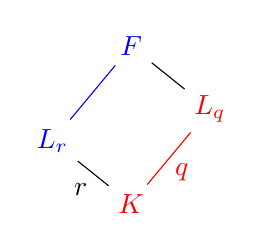
\begin{tikzpicture}

            \node [red] (Q1) at (0,0) {$K$};
            \node [red] (Q2) at (1,1.2) {$L_q$};
            \node [blue] (Q3) at (0,2) {$F$};
            \node [blue] (Q4) at (-1,0.8) {$L_r$};
        
            \draw [red] (Q1)--(Q2) node [pos=0.8, below,inner sep=0.25cm] {$q$};
            \draw (Q1)--(Q4) node [pos=0.9, below,inner sep=0.25cm] {$r$};
            \draw [blue] (Q3)--(Q4);
            \draw (Q2)--(Q3);
        
        \end{tikzpicture}
        \caption[short]{Subfields of a $C_{pq}$-extension}
    \end{figure}

    Again, the result follows immediately from the table and \eqref{eqn_local_contr}.
    
\end{proof}

We are finally ready to prove the main result of this section, from which Theorem \ref{thm_consistent_cyclic} will follow. 

\begin{lemma}\label{lem_Cd_odd}
    Let $d$ be a composite, odd squarefree integer and let $F/K$ be a Galois extension of number fields such that $\Gal(F/K)=C_{d}$. Let $E/\QQ$ be an elliptic curve with semistable reduction at $2$ and $3$ and let $L_k$ be the intermediate fields such that $\Gal(F/L_k)=C_{d/k}$. If 
    $$\Theta_d=\sum_{k\mid d}\mu(k)C_k\in B(C_d),$$
    then $C(\Theta_d)\in\QQss$.
\end{lemma}

\begin{proof}
    Let $n$ be the number of distinct prime numbers dividing $d$, so that $d=p_1\ldots p_n$ for some distinct odd primes $p_i$. We prove this result by induction. The base case for $n=2$ is the content of Lemma \ref{lem_Cpq}. Assume that the result holds for squarefree cyclic Galois extensions with $n-1$ prime factors and consider the two sets of subgroups
    $$\mathcal{A}=\{C_k:p_n\mid k\}\quad\text{and}\quad\mathcal{B}=\{C_k:p_n\nmid k\},$$
    which are clearly a partition of subgroups of $C_d$. Furthermore, the fields $\{F^{C_k}:C_k\in\mathcal{A}\}$ are precisely the intermediate fields of $L_{d/p_n}/K$, while the fields $\{F^{C_k}:C_k\in\mathcal{B}\}$ are the intermediate fields of $F/L_{p_n}$.
    Let 
    $$\Theta_\mathcal{A}=\sum_{H\in\mathcal{A}}\mu(|H|/p_n)H\quad\text{and}\quad\Theta_\mathcal{B}=\sum_{H\in\mathcal{B}}\mu(|H|)H$$
    and we note that
    \begin{equation}\label{eqn_theta}
        \Theta_d=\sum_{k\mid d}\mu(k)C_k=\sum_{p_n\nmid k\mid d}\mu(|C_k|)C_k-\sum_{p_n\mid k\mid d}\mu(|C_k|/p_n)C_k=\Theta_\mathcal{B}-\Theta_\mathcal{A}.
    \end{equation}
    Since $\Gal(L_{d/p_n}/K)=\Gal(F/L_{p_n})=C_{d/p_n}$, it follows from the inductive hypothesis applied to $L_{d/p_n}/K$ and $F/L_{p_n}$ that $C(\Theta_\mathcal{A}),C(\Theta_\mathcal{B})\in\QQss$, and therefore
    $$C(\Theta_d)=\frac{C(\Theta_\mathcal{B})}{C(\Theta_\mathcal{A})}\in\QQss,$$ 
    as desired.
    \begin{figure}[!ht]
        \centering
        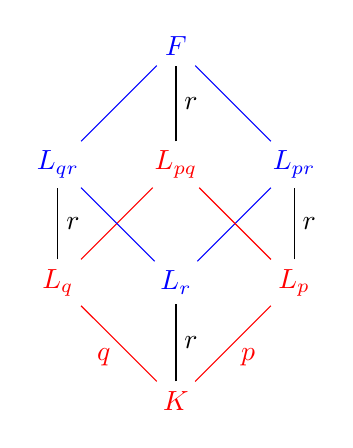
\begin{tikzpicture}

            \node [red] (Q1) at (0,0) {$K$};
            \node [red] (Q2) at (-1.5,1.5) {$L_q$};
            \node [blue] (Q3) at (0,1.5) {$L_r$};
            \node [red] (Q4) at (1.5,1.5) {$L_p$};
            \node [blue] (Q5) at (-1.5,3) {$L_{qr}$};
            \node [red] (Q6) at (0,3) {$L_{pq}$};
            \node [blue] (Q7) at (1.5,3) {$L_{pr}$};
            \node [blue] (Q8) at (0,4.5) {$F$};

            \draw [red] (Q1)--(Q2) node [pos=0.7, below,inner sep=0.25cm] {$q$};
            \draw [red] (Q1)--(Q4) node [pos=0.7, below,inner sep=0.25cm] {$p$};
            \draw (Q1)--(Q3) node [pos=0.5, right,inner sep=0.1cm] {$r$};
            \draw (Q2)--(Q5) node [pos=0.5, right,inner sep=0.1cm] {$r$};
            \draw (Q2)--(Q6) [red];
            \draw (Q3)--(Q5) [blue];
            \draw (Q3)--(Q7) [blue];
            \draw (Q4)--(Q6) [red];
            \draw (Q4)--(Q7) node [pos=0.5, right,inner sep=0.1cm] {$r$};
            \draw (Q5)--(Q8) [blue];
            \draw (Q6)--(Q8) node [pos=0.5, right,inner sep=0.1cm] {$r$};
            \draw (Q7)--(Q8) [blue];
        
        \end{tikzpicture}
        \caption[short]{Partition of $n=3$ into $n=2$. Red fields are in $\mathcal{A}$ while blue fields are in $\mathcal{B}$.}
    \end{figure}
\end{proof}

The proof of Theorem \ref{thm_consistent_cyclic} for odd $d$ is now straightforward.

\begin{proof}[Proof of Theorem \ref{thm_consistent_cyclic} for odd $d$]
    The proof is divided into two cases depending on whether $d$ is the power of a prime or not. Suppose first that $d$ is not, so that $\rad(d)$ is a squarefree \textbf{composite} number. Then $\Theta_d=\sum_{k\mid d}\mu(k)C_k\in B(C_d)$ is the $\psi_d$-relation of a faithful character of $C_d$. The subgroups appearing on $\Theta_d$ are the subgroups of $C_{\rad(d)}$ and therefore by Lemma \ref{lem_Cd_odd} applied to the $C_{\rad(d)}$ extension $F/F^{C_{\rad(d)}}$, it follows that 
    $$C(\Theta_d)\in\QQss,$$ and therefore it is the norm of an element for any quadratic extension of $\QQ$. 

    If $d=q^n$ for some odd prime $q$ and $n\geq1$, then Lemma \ref{lem_relation} shows that $\Theta_d=C_1-C_q$ is the $\psi_d$-relation of a faithful character of $C_d$. Lemma \ref{lem_Cp} applied to the $C_q$ extension $F/F^{C_q}$ proves that 
    $$C(\Theta_d)=\frac{C(C_1)}{C(C_q)}\in N_{\QQ(\sqrt{q^*})/\QQ}(\QQ(\sqrt{q^*})^{\times}).$$ 
    By Lemma \ref{lem_subfields} this is the only quadratic subfield of $\QQ(\zeta_{q^n})$, so the result follows.
\end{proof}

 
\subsubsection{Even Cyclic Extensions}
More care is required to prove Theorem \ref{thm_consistent_cyclic} for even $d$. This difficulty mainly lies in the case when $d$ is only divisible by one odd prime $q$. Consequently, we break down the proof into three distinct cases according to the number of odd prime divisors of $d$. If $d$ has more than one odd prime divisor, then the result follows without much work from Lemma \ref{lem_Cd_odd}, so we prove this first.

\begin{proof}[Proof of Theorem \ref{thm_consistent_cyclic} for even $d$ with more than one odd prime divisor]
    By Remark \ref{rem_radical}, recall that the subgroups present in $\Theta_d$ are precisely those such that $C_k\leq C_{\rad(d)}$, and so following a similar idea to Lemma \ref{lem_Cd_odd}, we define
    $$\mathcal{A}=\{C_k :2\mid k\mid\rad(d)\}\quad\text{and}\quad\mathcal{B}=\{C_k:2\nmid k\mid\rad(d)\},$$
    together with
    $$\Theta_\mathcal{A}=\sum_{H\in\mathcal{A}}\mu(|H|/2)H\quad\text{and}\quad\Theta_\mathcal{B}=\sum_{H\in\mathcal{B}}\mu(|H|)H. $$ 
    For each $k\mid d$, let $L_k=F^{C_{d/k}}$ be the unique subfield of degree $k$ over $K$. The fields $\{F^{C_k}:C_k\in\mathcal{A}\}$ are the intermediate fields of $L_{d/2}/L_{d/\rad(d)}$ and the fields $\{F^{C_k}:C_k\in\mathcal{A}\}$ are the intermediate fields of $F/L_{2d/\rad(d)}$. However, note that 
    $$\Gal(L_{d/2}/L_{d/\rad(d)})=\Gal(F/L_{2d/\rad(d)})=C_{\rad(d)/2},$$
    and by assumption $\rad(d)/2$ is an odd number with more than one prime factor. Then Lemma \ref{lem_subfields} applied to $L_{d/2}/L_{d/\rad(d)}$ and $F/L_{2d/\rad(d)}$ gives $\Theta_\mathcal{A},\Theta_\mathcal{B}\in\QQss$. The calculation in \eqref{eqn_theta} shows that $\Theta_d=\Theta_\mathcal{B}-\Theta_\mathcal{A}$ and therefore 
    $$C(\Theta_d)=\frac{C(\Theta_\mathcal{B})}{C(\Theta_\mathcal{A})}\in\QQss$$
    is the norm of any quadratic extension.
\end{proof}

If $d$ has no odd primes factors, then $d=2^l$ for some $l\geq1$. In that case, we assume in Theorem \ref{thm_consistent_cyclic} that $E$ is semistable, and the proof under this assumption is short. 

\begin{proof}[Proof of Theorem \ref{thm_consistent_cyclic} for $d=2^l$ and semistable $E$]

    If $l=1$, then $\QQ(\zeta_2)=\QQ$, and there is nothing to prove, so assume that $l\geq2$. If $\Gal(F/\QQ)=C_{2^l}$, then 
    $$C(\Theta_d)=\frac{C(C_1)}{C(C_2)}=\frac{C_{E/F}}{C_{E/L_{2^{l-1}}}},$$
    and $F/L_{2^{l-1}}$ is a $C_2$ extension. Importantly, we note that Table \ref{table_Cp} also applies for $q=2$, and therefore $\Cp(\Theta_d)$ is a rational square up to factors of $2$ for any prime $\pp$ of $L_{2^{l-1}}$. Lemma \ref{lem_subfields} shows that the only subfields of $\QQ(\zeta_{2^l})$ are $\QQ(i),\QQ(\sqrt{2})$ and $\QQ(\sqrt{-2})$, and since
    $$2=\Norm_{\QQ(i)}(1+i)=\Norm_{\QQ(\sqrt{-2})}(2)=\Norm_{\QQ(\sqrt{2})}(2+\sqrt{2}),$$
    it follows that $\Cp(\Theta_d)$ is a norm from every quadratic subfield of $\QQ(\zeta_{2^l})$, and the result follows.
\end{proof}

The remaining of this section is therefore devoted to the case when $d$ is divisible by one odd prime $q$, so $d=2^mq^n$. 
%When $d$ has this form, then $\Theta_d=C_1-C_2-C_q+C_{2q}$ and therefore fix $\Theta_d$ to have this expression for the remaining of this section. 
Recall that the quadratic subfields of $\QQ(\zeta_{2^mq^n})$ depend on whether $m=1$, $m=2$ or $m\geq 3$. Consequently, we prove three results that will be essential to prove the general version of each different case. The first covers the case $m=1$.

\begin{lemma}\label{lem_C2p}
    Let $q$ be an odd prime and let $F/K$ be a Galois extension of number fields such that $\Gal(F/K)=C_{2q}$ and let $L_k=F^{C_{2q/k}}$ be the intermediate fields such that $[L_k:K]=k$. Let $E/\QQ$ be an elliptic curve and let $\Theta_{2q}=C_{2q}-C_q-C_2+C_1\in B(C_{2q})$. Then
    $$C(\Theta_{2q})=\frac{C_{E/F}C_{E/K}}{C_{E/L_2}C_{E/L_q}}$$
    is a norm from $\QQ(\sqrt{q^*})$.
\end{lemma}

\begin{proof}
    Similarly to the proofs of Lemma \ref{lem_Cp} and \ref{lem_Cpq}, let $\pp$ be a prime in $K$ and assume that $\Delta_E=\Delta_{E,\pp}^{\min}$. The splitting behaviour of a prime $\pp$ in $K$ is again determined by $e_\pp$ and $f_\pp$ and therefore if $\pp$ has multiplicative reduction $\Dp(\Theta_{2q})=1$ and the following table records $\Tp(\Theta_{2q})$.

    \begin{table}[!ht]
        \centering
        \begin{tabular}{|l|l|l|l|l|l|l|}
        \hline
        $e_\pp$ & $f_\pp$  & $\Tp(C_{2q})$ & $\Tp(C_2)$ & $\Tp(C_q)$ & $\Tp(C_1)$ & $\Tp(\Theta_{2q})$ \\ \hline
        $1$ & $1$ & $n;\tilde{n}$ & $n^q;\tilde{n}^q$ & $n^2;\tilde{n}^2$ & $n^{2q};\tilde{n}^{2q}$ & $\square$ \\ \hline
        $1$ & $q$ & $n;\tilde{n}$ & $n;\tilde{n}$ & $n^2;\tilde{n}^2$ & $n^2;\tilde{n}^2$ & $\square$ \\ \hline
        $1$ & $2$ & $n;\tilde{n}$ & $n^q;\tilde{n}^q$ & $n;n$ & $n^q;n^q$ & $\square$ \\ \hline
        $1$ & $2q$ & $n;\tilde{n}$ & $n;\tilde{n}$ & $n;n$ & $n;n$ & $\square$ \\ \hline
        $q$ & $1$ & $n;\tilde{n}$ & $qn;\tilde{n}$ & $n^2;\tilde{n}^2$ & $q^2n^2;\tilde{n}^2$ & $q\square;\square$ \\ \hline
        $q$ & $2$ & $n;\tilde{n}$ & $qn;\tilde{n}$ & $n;n$ & $qn;n$ & $\square$ \\ \hline
        $2$ & $1$ & $n;\tilde{n}$ & $n^q;\tilde{n}^q$ & $2n;1$ & $2^qn^q;1^q$ & $\square$ \\ \hline
        $2$ & $q$ & $n;\tilde{n}$ & $n;\tilde{n}$ & $2n;1$ & $2n;1$ & $\square$ \\ \hline
        $2q$ & $1$ & $n;\tilde{n}$ & $qn;\tilde{n}$ & $2n;1$ & $2qn;1$ & $\square$ \\ \hline
        \end{tabular}
        \caption{Contribution of multiplicative reduction primes in a $C_{2q}$ extension.}
    \end{table}

    Since $q$ is a norm from $\QQ(\sqrt{q^*})$, then $\Tp(\Theta_{2q})$ is also a norm. Now assume that $\pp$ has additive reduction and let $p\ZZ=\pp\cap\QQ$. We first consider the contribution of the Tamagawa numbers. Note that $L_q/K$ and $F/L_2$ are $C_q$ extensions and therefore $\Tp(\Theta_{2q})\in\QQss$ if $q\neq 3$ and a square up to factors of $3$ if $q=3$. In either case, $\Tp(\Theta_{2q})$ is a norm from $\QQ(\sqrt{q^*})$.

    Finally, to compute $\Dp(\Theta_{2q})$, let $n=\nu_\pp(\Delta_{E,\pp}^{\min})$ and note that all terms cancel unless $\pp$ ramifies in $F$. If $e_\pp=2$, then
    \begin{equation}\label{eqn_ep=2}
        \Dp(C_{2q})=\Dp(C_2)=1,\quad \Dp(C_q)=N(\pp)^{\floor{\frac{2n}{12}}}\quad\text{and}\quad \Dp(C_1)=N(\pp)^{q\floor{\frac{2n}{12}}},
    \end{equation}
    and therefore $D(\Theta_{2q})=N(\pp)^{(q-1)\floor{n/6}}\in\QQss$, a rational square. If $q\mid e_\pp$, then $q\mid N(\pp)-1$ by Proposition \ref{prop_totally_ramified}, and the reasoning is now identical to Lemma \ref{lem_Cp}. Write $N(\pp)=p^s$ for some $s\geq1$ and note that $\Dp(\Theta_{2q})\in\QQss$ if $s$ is even. Hence, we assume that $s$ is odd. In this case, $p=q$ if $(L_q)_\fP/K_\pp$ is wildly ramified and $p$ splits in $\QQ(q^*)$ if $(L_q)_\fP/K_\pp$ is tamely ramified. In either case, by Corollaries \ref{p-norm} and \ref{cor_psplit_pnorm}, $p$ is a norm from $\QQ(\sqrt{q^*})$, and hence so is $\Dp(\Theta_{2q})$.
    The result follows again from \eqref{eqn_local_contr}.
\end{proof}

Following this, we state and prove the analogous result for $m=2$.

\begin{lemma}\label{lem_C4p}
    Let $q$ be an odd prime and let $F/K$ be a Galois extension of number fields such that $\Gal(F/K)=C_{4q}$ and let $L_k=F^{C_{4q/k}}$ be the intermediate fields such that $[L_k:K]=k$. Let $E/\QQ$ be an elliptic curve with semistable reduction at $2$ and $3$ and let $\Theta_{4q}=C_1-C_2-C_q+C_{2q}$. Then 
    $$C(\Theta_{4q})=\frac{C_{E/F}C_{E/L_2}}{C_{E/L_4}C_{E/L_{2q}}}$$
    is a norm from $\QQ(i),\QQ(\sqrt{q})$ and $\QQ(\sqrt{-q})$. Moreover, $\Tp(\Theta_{4q})\in\QQss$ for any prime $\pp$ in $K$, and $\Dp(\Theta_{4q})\in\QQss$ unless $E$ has additive reduction at $\pp$ and $\pp$ is totally ramified in $F/K$.
\end{lemma}

\begin{proof}
    All fields appearing in the product are intermediate fields of $F/L_2$, and $\Gal(F/L_2)=C_{2q}$. Let $\pp$ be a prime in $K$, let $\bar\pp\mid\pp$ be a prime above $\pp$ in $L_2$ and let $p\ZZ=\pp\cap\QQ$. Assume also that $\Delta_E=\Delta_{E,\pp}^{\min}$. Lemma \ref{lem_C2p} shows that if $E$ has multiplicative reduction over $\bar\pp$, $C_{\fP\mid\bar\pp}(\Theta_{4q})\in\QQss$ unless $e_{\bar\pp}=q$ and $f_{\bar\pp}=1$ over $F$. When this holds, $\bar\pp$ ramifies in $L_{2q}/L_2$ and is split in $L_4/L_2$, and this forces $\pp$ to split in $L_2/K$ too. Hence, $\pp=\bar\pp\bar\pp'$ for two \textbf{distinct} primes in $K$ that have the same local behaviour and therefore $\Cp(\Theta_{4q})=C_{\fP\mid\bar\pp}(\Theta_{4q})C_{\fP\mid\bar\pp'}(\Theta_{4q})=C_{\fP\mid\bar\pp}(\Theta_{4q})^2\in\QQss$, as desired.

    \begin{figure}[!ht]
        \centering
        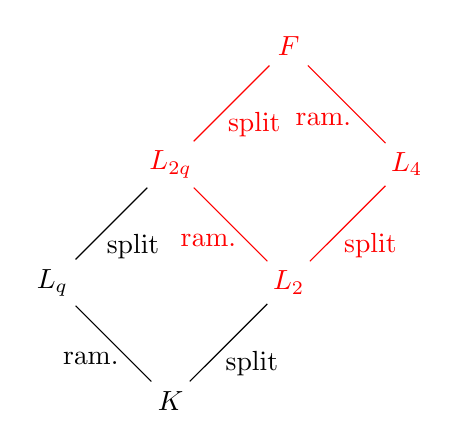
\begin{tikzpicture}

            \node (Q1) at (0,0) {$K$};
            \node (Q2) at (-1.5,1.5) {$L_q$};
            \node [red] (Q3) at (3,3) {$L_4$};
            \node [red] (Q4) at (1.5,1.5) {$L_2$};
            \node [red] (Q5) at (1.5,4.5) {$F$};
            \node [red] (Q6) at (0,3) {$L_{2q}$};
            

            \draw (Q1)--(Q2) node [pos=0.8, below,inner sep=0.4cm] {ram.};
            \draw (Q1)--(Q4) node [pos=0.8, below,inner sep=0.4cm] {split};
            \draw (Q2)--(Q6) node [pos=0.8, below,inner sep=0.4cm] {split};
            \draw [red] (Q3)--(Q5) node [pos=0.8, below,inner sep=0.4cm] {ram.};
            \draw [red] (Q4)--(Q6) node [pos=0.8, below,inner sep=0.4cm] {ram.};
            \draw [red] (Q6)--(Q5) node [pos=0.8, below,inner sep=0.4cm] {split};
            \draw [red] (Q4)--(Q3) node [pos=0.8, below,inner sep=0.4cm] {split};
        \end{tikzpicture}
        \caption[short]{\centering Field diagram for a $C_{4q}$ extension, together with the splitting\newline behaviour of a prime $\pp$ in $L_2$ with $e_\pp=q$ and $f_\pp=1$ over $F$.}
    \end{figure}

    Assume now that $E$ has additive reduction over $\bar\pp$. When $q=3$, controlling the Tamagawa numbers is lengthy, so we leave it for the end. We calculate first $\Dp(\Theta_{4q})$, which is $1$ unless $\bar\pp$ ramifies in $L/F_2$ (equivalently, $\pp$ ramifies in $L/K$). If $\pp$ is inert in $L_2/K$, then $N(\bar{\pp})\in\QQss$ and hence the size of all residues fields above $\pp$ are also squares and consequently $\Dp(\Theta_{4q})\in\QQss$ using Lemma \ref{lem_Dterms}. If $\pp=\bar\pp\bar\pp'$ splits, then $D_{\fP\mid\bar\fp}(\Theta_{4q})=D_{\fP\mid\bar\fp'}(\Theta_{4q})$, and therefore $\Dp(\Theta_{4_q})\in\QQss$ too. Finally, assume that $\pp=\bar\pp^2$ ramifies in $L_2/K$, which implies that $\bar\fp$ also ramifies in $L_4/L_2$. On the other hand, if $\bar\pp$ is unramified at $L_{2q}/L_2$, \eqref{eqn_ep=2} during the proof of Lemma \ref{lem_C2p} shows that $\Dp(\Theta_{4q})\in\QQss$ too. 

    We are therefore left with the case where $\pp$ is totally ramified in $F/K$, and Proposition \ref{prop_totally_ramified} implies that $4q\mid N(\pp)-1$. If we let $n=\nu_{\pp}(\Delta_{E,\pp}^{\min})$, Lemma \ref{lem_Dterms} implies that 
    \begin{equation*}\label{eqn_DtermsC4p}
        \Dp(\Theta_{4q})=N(\pp)^{\floor{\frac{n}{6}}-\floor{\frac{n}{3}}-\floor{\frac{qn}{6}}+\floor{\frac{qn}{3}}}.
    \end{equation*}
    Again, the parity of the expression only depends on $q,n\pmod{12}$. One can easily check that for $n\in\{2,3,4,6,8,9,10\}$ and $q\in\{1,5,7,11\}$, the above expression is a square unless $q\equiv 3\pmod{4}$ and $n$ is odd, so we assume this is the case. Write $N(\pp)=p^s$ for some $s\geq1$, which satisfies $p^s\equiv1\pmod{4q}$. If $s$ is even, then $\Dp(\Theta_{4q})\in\QQss$, so assume that $s$ is odd. Since $p^s\equiv1\pmod{4}$, this implies that $p\equiv1\pmod{4}$ and hence $p$ is a norm from $\QQ(i)$, which implies that $\Dp(\Theta_{4q})$ is a norm from $\QQ(i)$ too. Furthermore, the fact that $p^s\equiv1\pmod{4q}$ implies that
    $$\left(\frac{-q}{p}\right)=\left(\frac{q}{p}\right)=\left(\frac{p}{q}\right)=\left(\frac{p^s}{q}\right)=1,$$
    and therefore $p$ splits both in $\QQ(\sqrt{q})$ and $\QQ(\sqrt{-q})$. Since $q\equiv3\pmod{4}$, both fields have odd class number (Theorem \ref{thm_class_number}), and hence $p$ and $\Dp(\Theta_{4q})$ are norms from $\QQ(\sqrt{q})$ and $\QQ(\sqrt{-q})$ as desired. 

    Finally, we discuss Tamagawa numbers. Note that $L_{2q}/L_2$ and $F/L_4$ are $C_q$ extensions and therefore by Lemma \ref{lem_Cp} it follows that $\Dp(\Theta_{4q})\in\QQss$ if $q\neq3$. If $q=3$, it is also the case that $\Dp(\Theta_{4q})\in\QQss$, but more work is required. We prove this as a separate lemma, from which the result follows.    
\end{proof}

\begin{lemma}
    Let $L/K$ be a Galois extension of number fields with $\Gal(L/K)=C_{12}$ and let $L_k=F^{C_{12/k}}$ be the intermediate fields such that $[L_k:K]=k$. Let $E/\QQ$ be an elliptic curve and let $\pp$ be a prime in $K$ not dividing $2$ or $3$ such that $E$ has potentially good reduction at $\pp$. If $\Theta_{12}=C_1-C_2-C_3+C_6\in B(C_{12})$, then $$\Tp(\Theta_{12})=\frac{\Tp(E/F)\Tp(E/L_2)}{\Tp(E/L_6)\Tp(E/L_4)}\in\QQss.$$
\end{lemma}
\begin{proof}
    Let $\bar\pp$ be a prime in $L_2$ above $\pp$ and let $n=\nu_{\bar\pp}(\Delta_{E,\bar\pp}^{\min})$ be the minimal discriminant of $E$ at $\bar\pp$. If $\pp$ is unramified in $L_3/K$, then so is $\bar\pp$ in $L_6/L_2$ and the primes above them in $F/L_4$. From Lemma \ref{lem_Cp}, we know that that the product of Tamagawa numbers in unramified $C_3$ extensions is a square, so assume that $\pp$ ramifies in $L_3/K$.

    The proof is now divided in three cases, depending on the splitting behaviour of $\pp$ in $L_2$. If $\pp$ splits in $L_2/K$, then $\pp=\bar\pp\bar\pp'$ where $\bar\pp$ and $\bar\pp'$ have the same local behaviour. Therefore, $T_{\fP\mid\pp}(\Theta_{12})=T_{\fP\mid\bar\pp}(\Theta_{12})T_{\fP\mid\bar\pp'}(\Theta_{12})\in\QQss$. 
    
    Next, suppose that $\pp$ is inert in $L_2/K$, which implies that $\bar\pp$ is either inert or ramified in $L_4/L_2$. Let $\fP$ be the prime in $L_4$ above $\bar\pp$. If $\bar\pp$ is inert in $L_4/L_2$, then the valuation of the minimal discriminant of $E$ at $\fP$ is also $n$ and the splitting behaviour of $\bar\pp$ in $L_6/L_2$ coincides with the splitting behaviour of $\fP$ in $F/L_4$. Hence, 
    $$\frac{\Tp(E/F)}{\Tp(E/L_4)}=\frac{\Tp(E/L_6)}{\Tp(E/L_2)},$$
    and therefore $\Tp(\Theta_{12})=1$. The case where $\bar\pp$ is ramified in $L_4/L_2$ is more subtle. We have already seen that in ramified $C_3$ extensions we cannot obtain factors of $2$. Upon inspection of Lemma \ref{lem_add_tam}, one can easily show that the Tamagawa numbers cancel out if $\gcd(n,12)\in\{3,4,6,12\}$, so we only need to consider the case $\gcd(n,12)=2$. Since $\Gal((L_4)_\fP/K_\pp)=C_4$ and $e_{\fP\mid\pp}=f_{\fP\mid\pp}=2$, Lemma \ref{lem_notthree} shows that $\sqrt{B}\not\in F_{\fP}$ and therefore $c_\fP(E/F)=1$, which imples that $\Dp(\Theta_{12})\in\QQss$.

    Finally, assume that $\pp$ ramifies in $L_2/K$ so that $\pp=\bar\pp^2$. This immediately implies that $\bar\pp$ also ramifies in $L_4/L_2$, and therefore $\pp$ is totally ramified in $F/K$. As mentioned above, the Tamagawa numbers cancel unless $\gcd(n,12)=2$. However, recall that $E$ has potentially good reduction at $\pp$, and since $\pp=\bar\pp^2$ ramifies, then the valuation of the minimal discriminant at $\pp$ is $n/2$ or $(n+12)/2$. But then $\gcd(\nu_\pp(\Delta_{E,\pp}^{\min}),12)=\gcd(n/2,12)=1$, a contradiction. Hence, $\Tp(\Theta_{12})\in\QQss$ as desired.
\end{proof}

Finally, we state and prove the last result, from which the case $m\geq3$ follows easily. One needs to check that the product of local factors is the norm of many quadratic subfields; thankfully, Lemma \ref{lem_C4p} has done most of work required.

\begin{lemma}\label{lem_C8p}
    Let $q$ be an odd prime and let $F/K$ be a Galois extension of number fields such that $\Gal(F/K)=C_{8q}$ and let $L_k=F^{C_{8q/k}}$ be the intermediate fields such that $[L_k:K]=k$. Let $E/\QQ$ be an elliptic curve with semistable reduction at $2$ and $3$ and let $\Theta_{8q}=C_1-C_2-C_q+C_{2q}$. Then 
    $$C(\Theta_{8q})=\frac{C_{E/F}C_{E/L_4}}{C_{E/L_8}C_{E/L_{4q}}}\in\QQss.$$
    %is a norm from $\QQ(\sqrt{D})$ for each $D\in\{-1,\pm2,\pm q,\pm 2q\}$.
\end{lemma}

\begin{proof}
    We prove the result locally for all primes in $L_2$, and note $\Gal(F/L_2)=4q$. Let $\bar\pp$ and assume that $\Delta_E=\Delta_{E,\bar\pp}^{\min}$. Since the relation $\Theta_{4q}=C_1-C_2-C_q+C_{2q}\in B(C_{4q})$ has the same fixed fields as $\Theta_{8q}$, by Lemma \ref{lem_C4p}, we know that $\Tpb(\Theta_{8q})\in\QQss$ for any $\bar\pp$ and $\Dpb(\Theta_{8q})\in\QQss$ too unless $\bar\pp$ is totally ramified in $F/L_2$ and $E$ has potentially good reduction at $\bar\pp$, so assume this is the case. If $\pp=\bar\pp\cap K$, then it also follows that $\pp$ is totally ramified in $F/K$ and $E$ has potentially good reduction at $\pp$. If $n=\nu_{\bar\pp}(\Delta_{E,\bar\pp}^{\min})$, then recall from Lemma \ref{lem_C4p} that 
    $$\Dpb(\Theta_{8q})=N(\bar\pp)^{\floor{\frac{n}{6}}-\floor{\frac{n}{3}}-\floor{\frac{qn}{6}}+\floor{\frac{qn}{3}}},$$
    and that the exponent is even unless $n$ is odd and $q\equiv 3\pmod{4}$. However, $\pp=\bar\pp^2$ is ramified in $L_2/K$ and therefore $n\equiv 2\nu_\pp(\Delta_{E,\pp}^{\min})\pmod{12}$. That is, $n$ is even and therefore $\Dpb(\Theta_{8q})\in\QQss$ as desired.
\end{proof}
%%% THIS IS ALL PROBABLY NOT NEEDED NOW
%Again, $\Dp(\Theta_{8q})$ does not change up to squares if $\Delta_{E}$ is reescaled so assume that $\Delta_{E}=\Delta_{E,\pp}^{\min}$. Under these assumptions, $\Dpb(\Theta_{8q})=\Dp(\Theta_{8q})$ is a power of $N(\pp)=N(\bar\pp)=p^s$ for some rational prime $p$ and $s\geq1$. If $s$ is even, then $\Dpb(\Theta_{8q})\in\QQss$, so assume that $s$ is odd. In addition, by Proposition \ref{prop_totally_ramified}, it follows that $p^s\equiv 1\pmod{8q}$. Since $s$ is odd and $(\ZZ/8\ZZ)^*=C_2\times C_2$, it follows that $p\equiv 1\pmod{8}$ and therefore
%\begin{equation}\label{eqn_psplitsin2}
%    \left(\frac{-1}{p}\right)=\left(\frac{2}{p}\right)=\left(\frac{-2}{p}\right)=1.
%\end{equation}
%Furthermore, since $p^s\equiv1\pmod{8s}$ and $s$ is odd, then 
%\begin{equation}\label{eqn_psplitsinq}
%    \left(\frac{-q}{p}\right)=\left(\frac{q}{p}\right)=\left(\frac{p}{q}\right)=1.
%\end{equation}
%Combining \eqref{eqn_psplitsin2} and \eqref{eqn_psplitsinq} together with multiplicativity of the Legendre symbol, it follows that $p$ splits in every quadratic subfield $\QQ(\sqrt{D})$ for $D\in\{-1,\pm2,\pm q,\pm2q\}$.


We are now ready to prove the remaining case of Theorem \ref{thm_consistent_cyclic}.

\begin{proof}[Proof of Theorem \ref{thm_consistent_cyclic} for $d$ even and with one odd prime factor.]
    In this case, write $d=2^mq^n$ for $n,m\geq 1$ and note that $\Theta_{d}=C_1-C_2-C_q+C_{2q}$ is the $\psi_d$-relation of a faithful character of $C_d$. If $m=1$, Lemma \ref{lem_C2p} applied to the $C_{2q}$ extension $F/F^{C_{2q}}$ shows that $C(\Theta_d)$ is a norm from $\QQ(\sqrt{q^*})$, which is the only subfield of $\QQ(\zeta_{2q^n})$ by Lemma \ref{lem_subfields}. If $m=2$, then Lemma \ref{lem_C4p} applied to the $C_{4q}$ extension $F/F^{C_{4q}}$ shows that $C(\Theta_{d})$ is a norm from $\QQ(i),\QQ(\sqrt{q})$ and $\QQ(\sqrt{-q})$, which are all quadratic subfields of $\QQ(\zeta_{4q^n})$. Finally, if $m\geq3$, Lemma \ref{lem_C8p} applied to $F/F^{C_{8q}}$ shows that $C(\Theta_{8q})\in\QQss$, which is the norm from any quadratic subfield. The result follows.
\end{proof}



\subsection{Norm Relations in Odd Order Extensions}\label{subsec-odd}

We now prove a result analogous to the previous section, but when $F / \bQ$ is any Galois extension of odd order. %The reason one would expect that our norm relations test never forces rank growth in this case is because root number computations do not, as we now show.

%\begin{lemma}
% Let $F / \bQ$ be an odd Galois extension with $G = \Gal(F / \bQ)$. Then $w(E / \bQ) = w(E / F^H)$ for all $H \leq G$. 
%\end{lemma}

%\begin{proof}
%Consider $H \leq G$ and intermediate field $F^H$. Then $\Ind_H^G \trivial \simeq \trivial \oplus \rho \oplus \rho^*$ for some non self-dual representation $\rho$ of $G$, since the only self-dual representation of an odd-order group is the trivial representation. Therefore by Proposition \ref{compute-root-twist}, $w(E / F^H) = w(E / F)w(E, \rho \oplus \rho^*)$ and $w(E, \rho \oplus \rho^*) = 1$. Hence $w(E / \bQ) = w(E / F^H)$ for all $H \leq G$. 
%\end{proof}

%Therefore once we assume that $\rk E / \bQ = 0$, the parity conjecture tells us that $\rk E / F^H$ is even for all $H \leq G$, which does not force it to be non-zero. 


\begin{thm}\label{odd-exts}
 Let $E / \bQ$ be an elliptic curve, $F / \bQ$ be an extension of odd order with Galois group $G$. 
 
Assume that $E$ has good or multiplicative reduction at $2$ and $3$. 
Take any representation $\rho$ of $G$ with quadratic subfield $\bQ(\sqrt{D}) \subset \bQ(\rho)$ and relation
\begin{equation*}\label{odd-exp} \repnorm{\rho}^{\oplus m} =
 \left(\bigoplus_{\mathfrak{g}\in\Gal(\QQ(\rho)/\QQ)}\rho^{\mathfrak{g}}\right)^{\oplus m }=\bigoplus_i\Ind_{F_i/\QQ}\mathds{1}\ominus\bigoplus_j\Ind_{F'_j/\QQ}\mathds{1}
\end{equation*}
 as in Theorem \ref{thm_positive_rank}. Then
 \[ \frac{\prod_i C_{E/F_i}}{\prod_j C_{E/F_j'}}  \in 
    \begin{cases}
        N_{\bQ(\sqrt{D}) / \bQ}(\bQ(\sqrt{D})^{\times}) & m \ \text{odd}, \\
        (\bQ^{\times})^2 & m \ \text{even}.
    \end{cases} \] 
    In other words, one cannot use Theorem \ref{thm_positive_rank} to conclude that $E / F$ must have positive rank. 
\end{thm}

As in Remark \ref{rephrase-thm}, replacing $\rho$ by the sum of its conjugates by elements of $ \Gal(\bQ(\rho) / \bQ(\sqrt{D}))$, we may assume that $\bQ(\rho) = \bQ(\sqrt{D})$. We take $D \in \bZ \backslash \{0,1 \}$ to be squarefree.

The product of terms we are computing is $C(\Theta)$, where $C \colon \B(G) \to \bQ^{\times}$ is given by $C \colon H \mapsto C_{E / F^H}$, and $\Theta$ is any $\rho$-relation.
We break up the function $C$ into $C = \prod_p C_{\fP \mid p} = \prod_p T_{\fP \mid p} \cdot D_{\fP \mid p}$, ranging over primes $p \in \bQ$,
as defined in Notation \ref{not_contr_fns}.
We showed that
\begin{equation*}\label{Dp-loc}
C_{\fP \mid p} = (D_p, C_v)
\end{equation*}
where $C_v$ is a function on $\B(D_p)$ sending $H \mapsto C_v(E / F_w^H)$, for $D_p = \Gal(F_w / \bQ_p)$. The following result will allow us to apply some results from $\S$\ref{sec-norm-rels}.

\begin{thm}\label{odd-c-brauer}
    When $D_p$ has odd order, $C_v(\Psi) \in (\bQ^{\times})^2$ for any Brauer relation $\Psi \in \B(D_p)$. 
\end{thm}

\begin{proof}
    This follows from \cite[Theorem 2.47]{reg-const} and \cite[Theorem 3.2  (Tam)]{reg-const}.
\end{proof}

\begin{cor}
It is enough to prove Theorem \ref{odd-exts} when $m$ is the order of $\repnorm{\rho}$ in $\C(G)$. Thus we need to prove that, given any $
\Theta \in \B(G)$ such that $\bC[\Theta] \simeq \repnorm{\rho}^{\oplus m}$, $\Theta$ is a norm relation for the function $C$. 
\end{cor}

\begin{proof}
    Since $\bQ(\rho)$ is quadratic, we have that rational squares are norms from $\bQ(\rho)$. As $G$ is odd, any choice of $D_p$ is odd. It follows from Theorem \ref{odd-c-brauer} that $C(\Psi) \in (\bQ^{\times})^2$ for all Brauer relations $\Psi \in \B(G)$. Therefore by Proposition \ref{min-to-all}, it is enough to prove Theorem \ref{odd-exts} when $m$ is the order of $\repnorm{\rho}$ in $\C(G)$. Then $m$ divides $|G|$, hence is odd.
\end{proof}

Let $\tau$ be the generator of $\Gal(\bQ(\sqrt{D}) / \bQ)$.
Let $\ff$ be the smallest integer such that $\bQ(\sqrt{D}) \subset \bQ(\zeta_{\ff})$. Then $\ff \mid |G|$, hence is odd. By Remark \ref{conductor}, $\ff = |D|$ and $D \equiv 1 \pmod 4$. The following shows that it is only of interest to consider decomposition groups of exponent divisible by $\ff$.

\begin{cor}\label{rational-res-2}
    Let the exponent of $D_p$ be $b$. If $\ff \nmid b$, then $C_{\fP \mid p}(\Theta) \in (\bQ^{\times})^2$.
\end{cor}

\begin{proof}
    One has $\bQ(\rho) \subset \bQ(\zeta_b) \implies \ff \mid b$ by minimality of $\ff$. Since $\ff \nmid b$, we have $\bQ(\rho) \not\subset \bQ(\zeta_b)$, so $\bQ(\Res_{D_p} \rho) = \bQ$. The corollary then follows from Proposition \ref{rational-res} and Theorem \ref{odd-c-brauer}, noting that since $\C(D_p)$ is odd, multiplication by $2$ is injective. 
\end{proof}

Fix $\Theta = \sum_i n_i H_i \in \B(G)$ with $\bC[\Theta] \simeq \repnorm{\rho}^{\oplus m}$. We prove that at each prime $p$, $C_{\fP \mid p}(\Theta)$ is the norm of an element of $\bQ(\rho)$.  As observed, this depends on $D_p$ and $I_p$. As we deal with each local factor individually, we argue that one can take $D_p = I_p$.

\begin{lemma}\label{tam-up-to-square}
    Let $E / K$ be an elliptic curve. Let $K' / K$ be an extension of number fields odd degree, unramified at the place $v$ of $K$. Then $C_w(E / K') \equiv C_v(E / K) \mod (\bQ^{\times})^2$ for any place $w$ of $K'$ with $ w \mid v$. 
\end{lemma}

\begin{proof}
This is automatic for good reduction and split multiplicative reduction. It is also clear for non-split multiplicative reduction since the residue degree cannot be even (so the reduction type remains non-split at $w$). For additive reduction, see \cite[Lemma 3.12]{reg-const}.
\end{proof}

\begin{lemma}\label{DeqI}
    At a prime $p$, we may assume that $D_p = I_p$ when computing $C_{\fP \mid p}(\Theta)$. 
\end{lemma}

\begin{proof}
Let $p$ have residue degree $f_p$. Let $L / \bQ$ be a Galois extension of degree $f_p$ with cyclic Galois group, such that $p$ is inert in $L$. Further ensure that $F \cap L = \bQ$. Then $\Gal(FL / L) = G$. Let $F_i = F^{H_i}$ and $L_i = F_i L$.

Let $v$ be a place over $p$ in $F_i$. The extension $L_i / F_i$ is Galois, so $v$ is either split or inert in $L_i$.
We claim that $C_v(E / F_i) \equiv \prod_{w | v} C_w(E / L_i) \mod (\bQ^{\times})^2$. Indeed, the number of terms in the product on the right is odd, and by Lemma \ref{tam-up-to-square} $C_v(E / F_i) \equiv C_w(E / L_i) \mod (\bQ^{\times})^2$. 
Letting $C_{\fP \mid p}'$ be the function on $\B(G)$ defined as in \eqref{not_contr_fns} but with $\bQ$, $F$ replaced by $L$, $FL$, we see that $C_{\fP \mid p}'(\Theta) \equiv C_{\fP \mid p}(\Theta) \mod (\bQ^{\times})^2$. 
Thus it is equivalent to do our computation in $FL / L$, but here $p$ has residue degree $1$.
\end{proof}

To prove Theorem \ref{odd-exts}, we proceed by computing $C_{\fP \mid p}(\Theta)$ for each reduction type.

\subsubsection*{Good reduction}
If $E / \bQ$ has good reduction at $p$, then by Proposition \ref{prop_local_fns}(i), $C_{\fP \mid p} = 1$.

\subsubsection*{Multiplicative reduction}

\begin{lemma}
Let $E / \bQ_p$ have non-split multiplicative reduction. Then $C_{\fP \mid p}(\Theta) \in (\bQ^{\times})^2$.
\end{lemma}

\begin{proof}
Since $D_p = I_p$, all primes above $p$ have residue degree $1$. Moreover, the ramification degrees are always odd. Thus by Proposition \ref{prop_local_fns}(iii), $C_{\fP \mid p}  = (D_p, \alpha)$
where $\alpha$ is the constant function on $\B(D_p)$ with $\alpha \in \{1, 2\}$, depending on $v_p(\Delta)$ being even or odd. By Proposition \ref{const-fns}, it follows that $C_{\fP \mid p}(\Theta) \in (\bQ^{\times})^2$.
\end{proof}

Now suppose $E / \bQ_p$ has split multiplicative reduction. The reduction type remains split at all places above $p$ within sub-extensions of $F / \bQ$. Let $v_p(\Delta) = n$. Then by Proposition \ref{prop_local_fns}(ii), 
\[ C_{\fP \mid p} = (D_p, D_p, en). \]
Since the $n$ factor is constant, $(D_p, D_p, en)(\Theta) \equiv (D_p, D_p, e)(\Theta) \mod (\bQ^{\times}) ^2$ by Proposition \ref{const-fns} .

We have $D_p = I_p = P_p \ltimes C_l$, where $P_p \triangleleft I_p$ is wild inertia, and $C_l = I_p / P_p$ is the tame quotient. $C_l$ is a cyclic group, with $l \mid p^f - 1 = p - 1$. By Corollary \ref{rational-res-2}, we may consider such $D_p$ with exponent  $p^u l$ for some $u \geq 0$ such that $\ff \mid p^u l$. To compute $C_{\fP \mid p}(\Theta)$, we reduce to the tame quotient.

\begin{lemma}
Let $g \colon \B(C_l) \to \bQ^{\times}$ be defined by $H \mapsto [C_l \colon H] = \dim \bC[C_l / H]$. Let $\Psi = P_p \cdot \Res_{D_p} \Theta / P_p \in \B(C_l)$ Then $(D_p, D_p, e)(\Theta)$ and $g(\Psi)$ differ by a (possible) factor of $p$. 
\end{lemma}

\begin{proof}
%Now, $(D_p, D_p, e)(\Theta)$ is the product of ramification indices at primes above $p$. We separate the $p$-part and tame part of this expression.
Recall that the ramification index of a place $w$ above $p$ corresponding to the double coset $H_i x D_p$ has ramification degree $e_w = \frac{|I_p|}{|H_i \cap I_p^x|} =\frac{|I_p|}{|I_p \cap H^{x^{-1}}|}$.
This is the dimension of the permutation representation $\bC[D_p / D_p \cap H^{x^{-1}}]$.
Let  $D_p \cap H^{x^{-1}} = P' \ltimes C_a$ where $P' \leq P$ and $a | l$. Then the ramification index is $\frac{|P|}{|P'|}\cdot \frac{l}{a}$. 
Taking fixed points under wild inertia, one has the following isomorphism of $D_p$-representations  $$\bC[D_p / D_p \cap H^{x^{-1}}]^{P_p} \simeq \bC[D_p / P_p (D_p \cap H^{x^{-1}})] \simeq \bC[D_p / P_p \ltimes C_a].$$ This permutation representation has dimension $\frac{l}{a}$, so we've killed off the $p$-part. 
Then $$\bC[\Res_{D_p} \Theta]^{P_p} \simeq \left(\Res_{D_p} \rho^{\oplus m} \oplus \tau\left(\Res_{D_p}\rho^{\oplus m}\right)\right)^{P_p},$$
and we can consider these as representations of $D_p / P_p = C_l$.
It follows that $(D_p, D_p, e)(\Theta)$ differs from $g(\Psi)$ up to a (possible) factor of $p$. 
\end{proof}

Now we show that this factor of $p$ is a norm from $\fieldnorm{\rho}$.
Note that if $p = 2$ then $P_p = 1$ since $|P_p| \mid |G|$ which is odd. So we only need to consider this factor of $p$ for $p$ odd.

\begin{lemma}\label{p-norm-odd}
    Let $K = \bQ(\sqrt{D})$, with $\ff$ the smallest positive integer such that $K \subset \bQ(\zeta_{\ff})$. Suppose that $\ff$ is odd. Let $\ff \mid p^u l $, for some odd prime $p$, $u \geq 0$ and $l$ such that $p \equiv 1 \pmod l$. Then $p$ is the norm of an element from $K^{\times}$.
\end{lemma}

\begin{proof}
    Since $\ff$ is odd, one has $D = \prod_{q | \ff} q^*$, the product being taken over primes dividing $\ff$. Note that if $q \not= p$, then since $q \mid l$, we have $p \equiv 1 \pmod l \implies p \equiv 1 \pmod q$. By Corollary \ref{p-one-mod-disc},  $p$ is the norm of a principal fractional ideal of $K$, and by Theorem \ref{p-norm-elem-1} or Theorem \ref{p-norm-elem-2}, it is the norm of an element of $K$.
    %We show that $p$ has residue degree $1$ in the extended genus field $E^{+} = K(\{\sqrt{q^*} \colon q | \ff \})$ of $K$ ({\color{red} cf. appendix}).
    %If $q \not= p$ then $q \mid l$, so $p \equiv 1 \pmod l$. Therefore $p$ splits in any quadratic subfield of $E^{+}$ of discriminant not divisible by $p$. Else, $p$ ramifies in any quadratic subfield with discriminant divisible by $p$. Thus it is clear that $p$ has residue degree $1$ in $E^{+}$, hence also in the genus field $E$, and it follows from theorem \ref{p-principal} that $p$ is the norm of a principal ideal.  Else, we invoke theorem \ref{minus-one-norm}.
\end{proof}

\begin{cor}
Let $E / \bQ_p$ have split multiplicative reduction. Then $C_{\fP \mid p}(\Theta) \in \fieldnorm{\rho}$.
\end{cor}

\begin{proof}
By the previous two results, it is sufficient to show that $g(\Psi) \in \fieldnorm{\rho}$. Let $\phi = (\Res_{D_p} \rho)^{P_p}$, viewed as a representation on $D_p / P_p = C_l$. Then $\Psi$ is a $\phi$-relation. If $\ff \nmid l$ then $\bQ(\phi) = \bQ$. Therefore $\bC[C_l / \Psi] \simeq \phi^{\oplus 2}$, implying that $\Psi = 2\Psi'$ for some $\Psi' \in \B(C_l)$ with $\bC[C_l / \Psi'] = \phi$. Then $g(\Psi) = g(\Psi')^2 \in \fieldnorm{\rho}$. Otherwise, suppose that $\bQ(\phi) = \bQ(\rho)$. It follows from Proposition \ref{index-fn-trivial} that $g(\Psi) \in \fieldnorm{\rho}$.
\end{proof}

\subsubsection*{Additive reduction}

Now suppose that $E / \bQ_p$ has additive reduction. In this case, assume that $p \geq 5$
Write $D_p = \Gal(F_w / \bQ_p)$ for $w \mid p$ a place of $F$.

Again we have $D_p = P_p \ltimes C_l$ with $ l \mid p - 1$, and may assume that $\ff \mid p^u l$ where $p^u l $ is the exponent of $D_p$ by Corollary \ref{rational-res-2}. Let $n = v_p(\Delta_E)$. 

We will compute $D_{\fP \mid p}(\Theta)$ and $T_{\fP \mid p}(\Theta)$ separately. 
By Proposition \ref{prop_local_fns}(iv), (v)
\[ D_{\fP \mid p} = 
    \begin{cases}
        (D_p, D_p,\ p^{\floor{e_ /2}}) & \text{if } E / \bQ_p \text{ has potentially multiplicative reduction}, \\
        (D_p, D_p,\ p^{\floor{en /12}}) & \text{if } E / \bQ_p \text { has potentially good reduction}.
    \end{cases}
    \]
In either case, $D_{\fP \mid p}(\Theta) \in N_{\bQ(\rho) / \bQ}(\bQ(\rho)^{\times})$. Indeed, this takes values $1$ or $p$ in $\bQ^{\times} / (\bQ^{\times})^2$. But $p$ is a norm from $\bQ(\rho)$ by Lemma \ref{p-norm-odd}.

%\[ \left|\frac{\Delta_{E}}{\Delta_{E, w}^\min} \right|_w = p^{f_w 12 \cdot \floor{e_w n / 12}} \implies 
%       \left|\frac{\omega}{\omega_{w}^\min} \right|_w = p \]
\vspace{1em}

To compute $T_{\fP \mid p}(\Theta)$, since $p \geq 5$ we may write $E / \bQ_p$ as $E \colon y^2 = x^3 + A x + B$ and use the description from \cite{reg-const} for computing Tamagawa numbers, as detailed in Lemma \ref{tamagawa-num}. The discriminant of $E / \bQ_p$ is $\Delta = -16(4A^3 + 27 B^2)$. The case of potentially multiplicative reduction is almost immediate:

\begin{lemma}[Potentially multiplicative reduction]
    If $E / \bQ_p$ has reduction type $\I_{n}^{*}$ then $T_{\fP \mid p}(\Theta) \in (\bQ^{\times})^2$. 
\end{lemma}

\begin{proof}
Since we assume $D_p = I_p$, i.e. the residue degree is one, it follows that any subextension $L'$ of $F_{w} / \bQ_p$ satisfies $\sqrt{B} \in L' \iff \sqrt{B} \in \bQ_p$ and $\sqrt{\Delta} \in L' \iff \sqrt{B} \in \bQ_p$. 
Therefore $T_{\fP \mid p} = (D_p, \alpha)$ where $\alpha \in \{2, 4\}$ by Lemma \ref{lem_add_tam}. But then $(D_p, \alpha)(\Theta) \in (\bQ^{\times})^2$ by Proposition \ref{const-fns}.
\end{proof}

Now suppose that $E / \bQ_p$ has potentially good reduction. Recall from Lemma \ref{lem_add_tam} that if $L' / \bQ_p$ has ramification degree $e$, then the Kodaira type of $E / L'$ depends on $\gcd(e n, 12)$. Thus in a ramified extension of degree coprime to $12$, the Kodaira type is unchanged, and further if this extension is totally ramified (so the residue degree is $1$), the Tamagawa number is unchanged also. Thus when $3 \nmid |D_p|$, $T_{\fP \mid p} = (D_p, \alpha)$ for some constant $\alpha$. If we have type $\III$ or $\III^*$ or $\I_0^*$ then the Tamagawa number is still unchanged in any totally ramified extension of odd degree extension, even when the degree is divisible by $3$. Then the Proposition \ref{const-fns} implies the following lemma:

\begin{lemma}
    \
    \begin{enumerate}[(i)]
        \setlength\itemsep{0em}
        \item If $E / \bQ_p$ has potentially good reduction and $3 \nmid |D_p|$, then $T_{\fP \mid p}(\Theta) \in (\bQ^{\times})^2$.
        \item If $E / \bQ_p$ has potentially good reduction of type $\III$, $\III^*$, or $\I_0^*$, then $T_{\fP \mid p}(\Theta) \in (\bQ^{\times})^2$.
    \end{enumerate}
\end{lemma}

Thus we assume that $3 \mid |D_p|$. Since we assumed $p \geq 5$, we have $D_p = I_p = P_p \ltimes C_l$ with $3 \mid l$ and $p \equiv 1 \pmod l$.

\begin{lemma}
If $E / \bQ_p$ has Type $\II$ or Type $\II^*$ additive reduction and $3 \mid |D_p|$, then $T_{\fP \mid p}(\Theta) \in (\bQ^{\times})^2$. 
\end{lemma}

\begin{proof}
If $3 \mid |D_p|$ then there is a subextension $F'$ of $F_w / \bQ_p$ with $\Gal(F_w / F') = C_3$. Then Lemma \ref{lem_nottwo} implies that $\sqrt{\Delta} \in F'$. But $F' / \bQ_p$ has residue degree $1$, hence $\sqrt{\Delta} \in \bQ_p$. 

If $L' / \bQ_p$ is an odd degree extension that is divisible by $3$, then $E / L'$ has reduction type $I_0^*$. By Lemma \ref{tamagawa-num} the Tamagawa number of $E / L'$ is $2$ if $\sqrt{\Delta} \not\in \bQ_p$ and $1$ or $4$ if $\sqrt{\Delta} \in \bQ_p$. Therefore the Tamagawa number will be $1$ or $4$, which is a square.
On the other hand if $L' / \bQ_p$ is an extension of odd degree then the reduction type over $L'$ is $\II$ or $\II^*$ and the Tamagawa number is $1$. It follows that $T_{\fP \mid p}(\Theta)$ is a product of square terms, so is itself square.  
\end{proof} 

Now, if $E /\bQ_p$ has additive reduction of type $\IV$ or $\IV^*$, it attains good reduction over any totally ramified cyclic extension of degree divisible by $3$. This could result with $3$ coming up an odd number of times in $T_{\fP \mid p}(\Theta)$, when $\sqrt{B} \not\in \bQ_p$. 
%We show that for both types, one has $\sqrt{B} \in \bQ_p$. 
%Indeed, if $\delta = 4$, then $v_p(B) = 2$, and $v_p(A) \geq 2$. 
%\vspace{1em}
%In summary, 
%\begin{equation}
 %   \prod_{d ' \mid d} C(E / F_{\fp}^{D_{d'}})^{\mu(d / d')}
  %  = 
   % \begin{cases}
    %    1 & 3 \nmid d, \\
    %   1 & 3 \mid d, \delta \in \{0, 3, 6, 9\}, \\
    %    1 \cdot \square & 3 \mid d, \delta \in \{2, 10\}, \\
    %    3^a \cdot\square, a \in \{0,1\} & 3 \mid d, \delta \in \{4,8\}.
    %\end{cases}
%\end{equation}
%\begin{rem}
%   There's no reason why we can't get 3; see elliptic curve 441b1 with additive reduction at $7$ of type IV and Tamagawa number equal to $3$
%\end{rem}

%\textbf{If $D_p = C_l$ then we are able to finish our argument.} As in the proof of Proposition \ref{semi-stable-gd}, there exists $a_{l'} \in \bZ$ such that $\Res_{D_p}\Theta = \sum_{l' \mid l} a_{l'} \Psi_{l'}$ where $\Psi_{l'} \in \B(G)$ is such that $\bC[\Psi_{l'}] \simeq \chi_{l'}$, as in Example \ref{cyclic-relns}.

Recall from the proof of Proposition \ref{const-fns} that $\Res_{D_p} \Theta = \sum_i n_i \sum_{x \in H_i \backslash G / D_p} D_p \cap H^{x^{-1}}$, with $\sum_i n_i | H_i \backslash G / D_p|$ even. If $D_p = \Gal(F_w / \bQ_p)$, then the number of subextensions divisible by $3$ (i.e. the number of subextensions where we obtain good reduction ) corresponds to the number of subgroups with index divisible by $3$ in $\Res_{D_p}\Theta$. We compute this number to determine $\ord_3(T_{\fP \mid p}(\Theta))$ modulo squares.

Similarly to the split multiplicative case, we may pass to the tame quotient $C_p / P_p = C_l$. Indeed 

\[ 3 \mid  [D_p : D_p \cap H^{x^{-1}}] = \dim \bC [ D_p / D_p \cap H^{x^{-1}}] \iff 3 \mid \dim \bC[ D_p / D_p \cap H^{x^{-1}} ]^{P_p},\] 
since $3 \nmid|P_p|$. Therefore we may compute the number of subgroups divisible by $3$ in $\Psi = P_p \cdot \Res_{D_p} \Theta / P_p \in \B(C_l)$.  Let $h \colon \B(C_l) \to \bQ^{\times}$ be the function given by $H \mapsto \begin{cases} 3 & 3 \mid [C_l : H], \\ 1 & 3 \nmid [C_l : H]. \end{cases}$

\begin{prop}
   Suppose that $E / \bQ_p$ has additive reduction of Type $\IV$ or $\IV^*$, with $c_v(E / \bQ_p) = 3$.  Then $T_{\fP \mid p}(\Theta) \equiv h(\Psi) \mod (\bQ^{\times})^2$ and $T_{\fP \mid p}(\Theta) \in \fieldnorm{\rho}$. 
\end{prop}

\begin{proof}
The fact that $T_{\fP \mid p}(\Theta) \equiv h(\Psi) \mod (\bQ^{\times})^2$ has been observed above.
Let $\psi_3$ be an irreducible character of $D_p$ of order $3$. One has that $ \langle \Ind_{C_{l / l'}}^{C_l} \trivial , \psi_3 \rangle =  1$ when $3 \mid l'$ and is zero when  $3 \nmid l'$. 
Thus $$h(\Psi) = 3^{\langle \bC[C_l / \Psi], \psi_3 \rangle}.$$ As in the proof of Proposition \ref{index-fn-trivial}, write $\bC[C_l / \Psi] = \sum_{l' \mid l} a_{l'} \chi_{l'}$, where $\chi_{l'}$ is an irreducible rational character, of $C_l$ with kernel of index $l'$. Observe that $\langle \chi_{l'}, \psi_3 \rangle = 0$ unless $l' = 3$, in which case it is $1$. Therefore $h(\Psi) \equiv 3^{a_3} \mod (\bQ^{\times})^2$. In the proof of Proposition \ref{index-fn-trivial}, we showed that $a_3$ is even unless $\ff \mid 3$,  i.e. that $\bQ(\rho) = \bQ(\sqrt{-3})$. But then $3$ is a norm in $\bQ(\rho)$. Thus we see that in all cases $T_{\fP \mid p}(\Theta) \in N_{\bQ(\rho) / \bQ}(\bQ(\rho)^{\times})$. 
\end{proof}

We have observed that for all reduction types of $E / \bQ_p$, one has $C_{\fP \mid p} (\Theta) \in \fieldnorm{\rho}$, and so $C(\Theta) \in \fieldnorm{\rho}$, completing the proof of Theorem \ref{odd-exts}.

\qed

\begin{cor}\label{cor-odd-decomp}
    Let $G$ be a finite group, $\rho$ a character of $G$ with $\bQ(\rho)$ quadratic. Let $\Theta \in \B(G)$ be a $\rho$-relation. If $D_p \leq G$ is of odd order, then $C_{\fP \mid p}(\Theta) \in \fieldnorm{\rho}$.
\end{cor}

\begin{proof}
 Throughout this section our results only depended on the oddness of $D_p$.
\end{proof}


\newpage
\begin{appendices}
\section{Algebraic Number Theory Background}
%\subsection{Decompositions of primes in field extensions}
\subsection{Class field theory and genus fields}

In this section we introduce the concept of a genus field, as well as properties that will be useful for us.

Let $K$ be a number field. The \textbf{ideal class group} $\Cl_K = I_K / P_K$ is the group of fractional ideals modulo principal fractional ideals.
For an ideal $\fp$, we let $[\fp]$ denote its class in $\Cl_K$.

The \textbf{extended ideal class group} is the group $\Cl_K^{+} = I_K / P_K^{+}$, where
$P_K^{+}$ denotes the subgroup of principal fractional ideals with totally positive generator, i.e. ideals $\alpha \cO_K$ where $\sigma(\alpha) > 0$ for all real embeddings $\sigma \colon K \emb \bR$.

Note that $\Cl_K^{+}$ is the ray class group for the modulus $\fm$ of $K$ consisting of the product of all real places. The corresponding ray class field is known as the \textbf{extended Hilbert class field}, which we'll denote as $H^{+}$. This is the maximal extension of $K$ that is unramified at all finite primes. Let $H$ be the usual Hilbert Class field of $K$. Then one has $H \subset H^{+}$. Moreover, the index can be described in terms of the structure of $K$:

\begin{thm}\cite[Chapter VI, Section 3, Theorem 3.1]{Janusz}
    Let $r$ be the number of real primes of $K$. Let $U_K$, $U_K^{+}$ the group of units and totally positive units of $K$ respectively, Then 
    \[ [H^{+} \colon H] = 2^r [U_K \colon U_K^{+}]^{-1} .\]
\end{thm}
Observe that if $K$ has no real places, then $H^{+} = H$. For quadratic fields, the index depends on the norm of a fundamental unit:

\begin{cor}
    Let $K = \bQ(\sqrt{D})$ with $D$ a square-free positive integer. Let $\epsilon$ be a fundamental unit of $K$. Then $[H^{+} \colon H] = 1$ or $2$, according as $N_{K / \bQ}\left(\epsilon\right) = -1$ or $1$. 
\end{cor}


Fix $K = \bQ(\sqrt{D})$ for $D$ a squarefree integer. The (extended) Hilbert class field of $K$ need not be abelian over $\bQ$ (note that it is Galois over $\bQ$ by uniqueness of the (extended) Hilbert class field). However it can be useful to consider the maximal subfield of $H$ that is abelian over $\bQ$. 

\begin{defn}
    For any abelian extension $K / \bQ$, the \textbf{genus field} of $K / \bQ$ is the largest abelian extension $L / \bQ$ contained in $H$. The \textbf{extended genus field } is the largest abelian extension $L^{+} / \bQ $ contained in $H^{+}$.
\end{defn}

Let $\sigma \in \Gal(H^{+} / \bQ)$ be such that $\sigma|_{K}$ generates $\Gal(K / \bQ)$. $L$ has the following properties:

\begin{thm}\cite[Ch. VI, $\S$3, Theorem 3.3]{Janusz}\label{janusz-3.3}
    Let $K = \bQ(\sqrt{D})$.
    \begin{enumerate}
        \item $\Gal(H / L)$ is isomorphic to the subgroup of $C_K$ generated by the ideal classes of the form $[\sigma(\fU)\fU^{-1}]$, $\fU \in I_K$. 
        \item $\Gal(H / L) \simeq (C_K)^2$. 
    \end{enumerate}
\end{thm}

\begin{proof}[Proof sketch of 1.]
    Let $G = \Gal(H / \bQ)$. Then $L = H^{[G, G]}$ is the fixed field of the commutator subgroup of $G$. The Artin map induces an isomorphism $\varphi \colon C_K \to C \subset G$ with $\varphi(C_K) \simeq C = \Gal(H / K)$. One shows that $\varphi([\sigma(\fU)\fU^{-1}]) \in [G, C]$ and conversely that every commutator element in $[G, G]$ can be expressed as $\varphi([\sigma(\fU)\fU^{-1}])$ for some $\fU \in I_K$. 
\end{proof}

%Note that this says that every class $[\sigma(\fU) \fU^{-1}]$ is a square in $C_K$.
This allows us to deduce the following:

\begin{thm}\label{p-principal}
Let $p$ be a prime in $\bQ$. If the residue degree of $p$ in $L / \bQ$ is $1$, then $p$ is the norm of a principal fractional ideal in $K$. 
\end{thm} 

\begin{proof}
Let $\varphi \colon C_K \to \Gal(H / K)$ be the isomorphism induced by the Artin map. By Theorem \ref{janusz-3.3}, $\Gal(L / K) = \Cl_K / \left(\Cl_K\right)^2$ is abelian. Let $\fp$ be a prime of $K$ lying over $p$. Then $N_{K / \bQ}(\fp) = p$ and $\fp$ has residue degree $1$ in $L$. It follows that $\varphi([\fp])|_{L} = \Id$ so that $\varphi([\fp]) \in \Gal(H / L)$. Thus by Theorem \ref{janusz-3.3} there is a fractional ideal $\fU$ of $I_K$ such that 
$[\fp] = [\sigma(\fU)\fU^{-1}]$. Observe that $N_{K / \bQ}(\sigma(\fU)\fU^{-1}) = 1$. It follows that we can represent $[\fp]^n$ by a fractional ideal of norm $p$ for all $n \geq 1$. Since $\Cl_K$ is finite, this implies there is a principal fractional ideal in $K$ of norm $p$. 
\end{proof}

Observe that $C_K / (C_K)^2$ is an abelian group of exponent $2$. The following theorem describes its order:

\begin{thm}\cite[Ch VI, \S3, Theorem 3.9]{Janusz}
Suppose the discriminant of $K / \bQ$ has $t$ prime divisors. Then $C_K / (C_K)^2$ has order $2^{t-1}$ if $D < 0$ or if $D > 0$ and a unit of $K$ has norm $-1$. Otherwise, if $D > 0$ and all units of $K$ have norm $1$, it has order $2^{t - 2}$.
\end{thm} 

\begin{rem}\label{conductor}
    The conductor of $K / \bQ$ is a particular modulus for $K / \bQ$ ({\color{red} ref}). We denote the finite part of it by $\ff \in \bZ_{>0}$ . Then $\ff$ is the smallest positive integer such that $K \subset \bQ(\zeta_{\ff})$. For quadratic fields, one has that $\ff = |\Delta|$ where $\Delta$ is the discriminant of $K$ ({\color{red} ref}). Thus
\[ \ff = |\Delta| =  \begin{cases} |D| & D \equiv 1 \pmod 4, \\ 4|D| & D \not\equiv 1 \pmod 4. \end{cases} \]
\end{rem}

Our introduction of the extended genus field $L^{+}$ is mostly because it is easier to describe than $L$.

\begin{thm}\label{extended-genus}\cite[Ch VI, \S3, Theorem 3.10]{Janusz}
Let the discriminant of $K = \bQ(\sqrt{D})$ be $\Delta$ and suppose $|\Delta| = p_1 p_2 \cdots p_t$ where $p_2, \ldots p_t$ are odd primes, and $p_1$ is either odd or a power of $2$. Then the extended genus field of $K$ is 
    \[ L^{+} = \bQ(\sqrt{D}, \sqrt{p_2^*}, \ldots \sqrt{p_t^*}) = K(\sqrt{p_2^*}, \ldots \sqrt{p_t^*}), \] 
where 
\[ \begin{cases}
    p_i^* = p_i & \mathrm{if }\ p_i \equiv 1 \pmod 4, \\
    p_i^* = -p_i & \mathrm{if }\ p_i \equiv 3 \pmod 4
\end{cases}\]
\end{thm} 

\vspace{1em}

\begin{cor}\label{p-one-mod-disc}
    Let $p$ be an odd prime in $\bQ$, $K = \bQ(\sqrt{D})$ with discriminant $\Delta$ such that $|\Delta| = p_1 p_2 \cdots p_t$, as in Theorem \ref{extended-genus}. If $p \equiv 1 \mod {|\Delta|}$, then $p$ is the norm of a principal fractional ideal in $K$. 
    It is also the norm of a principal fractional ideal in $K' = \bQ({\sqrt{p^*D}})$.
\end{cor}

\begin{proof}
   Let $L^+ = \bQ(\sqrt{D}, \sqrt{p_2^*}, \ldots \sqrt{p_t^*})$ be the extended genus field of $K$, and $L$ the genus field. If $p$ has residue degree $1$ in $L^+ / \bQ$, then it has residue degree $1$ in $L / \bQ$, and the first result follows by Theorem \ref{p-principal}. 

   Note that $p$ splits in the quadratic subfields $\bQ(\sqrt{p_i^*})$ for $i = 2, \ldots t$, since $\legendre{p_i^*}{p} = \legendre{p}{p_i} = 1$, as $p \equiv 1 \pmod {\Delta} \implies p \equiv 1 \pmod {p_i}$ for $i = 2, \ldots t$. To show that $p$ splits in $L^+$ we just need to show that it also splits in $K$. 
   
   First suppose $D \equiv 1 \pmod 4$. Write $D = \prod_{i=1}^t p_i^*$. Then 
    \[ \legendre{D}{p} = \prod_{i = 1}^t \legendre{p_i^*}{p} = \prod_{i = 1}^t \legendre{p}{p_i} = 1. \]
    Thus $p$ splits in $K$.

    Now consider that $D \not\equiv 1 \pmod 4$. First assume $D \equiv 3 \pmod 4$. Write $D = -\prod_{i=2}^t p_i^*$. Then
    \[ \legendre{D}{p} = \legendre{-1}{p} \prod_{i = 2}^t \legendre{p_i^*}{p} = \legendre{-1}{p} = 1, \] 
    since $p \equiv 1 \pmod {|\Delta|}$ and $4 \mid |\Delta| \implies p \equiv 1 \pmod 4$. 

    Now assume that $2 \mid D$ so that $8 \mid |\Delta|$ and $p \equiv 1 \pmod 8$. Then $D = \pm 2 \prod_{i = 2}^t p_i^*$. Thus
    \[ \legendre{D}{p} = \legendre{\pm 1}{p} \legendre{2}{p}\prod_{i = 2}^t \legendre{p_i^*}{p} = 1 .\] 

    Let $L'^{+}$ be the extended genus field of $K'$. Now $p$ ramifies in $K'$, $\bQ(\sqrt{p^*})$. Using the calculations above, it is either split or ramified in all quadratic subfields of $L'^{+}$, and so has residue degree $1$ in $L'^{+}$, and the result follows. 
\end{proof}

We want to understand when $p \in N_{K / \bQ}(K^{\times})$. If $p$ is the norm of a principal fractional ideal in $K$, then $\pm p \in N_{K / \bQ}(K^{\times})$. If $K$ is imaginary, one must have $p \in N_{K / \bQ}(K^{\times})$. We can also arrive to the same conclusion when $K$ is real and $-1 \in N_{K / \bQ}(K^{\times})$. 

\begin{thm}\label{minus-one-norm}
Let $K = \bQ(\sqrt{D})$ with $D >0$ squarefree and suppose that all odd primes dividing $D$ are congruent to $1 \pmod 4$. Then $-1$ is the norm of an element of $K^{\times}$. 
\end{thm}

\begin{proof}
The condition on $D$ ensures that there exists $x$, $y \in \bQ$ such that $D = x^2 + y^2$. Therefore $-1 = (x / y)^2 - D(1/ y)^2$ so that $-1$ is the norm of the element $\frac{x}{y} + \frac{1}{y} \sqrt{D}$.
\end{proof}

Note that $-1$ being the norm of an element in $K$ does not ensure that $-1$ is the norm of a unit in $K$. The smallest counter-example is $K = \bQ(\sqrt{34})$. The element $\frac{5}{3} + \frac{1}{3}\sqrt{34}$ has norm $-1$, but there is no unit with norm $-1$. 

\begin{thm}\label{p-norm-elem-1}
    Let $K = \bQ(\sqrt{D})$ be a real quadratic field.  If $p$ is an odd prime such that $p \equiv 1 \pmod {|\Delta|}$, then $p$ is the norm of an element from $K$. 
\end{thm}

\begin{proof}
    We know that $p$ is the norm of a principal fractional ideal of $K$ by Corollary \ref{p-one-mod-disc}. 
    Therefore there exists integers $x$, $y$, $z$ such that $\pm p z^2 = x^2 - Dy^2$. 
    
    Suppose firstly that all odd primes dividing $D$ are congruent to $1 \pmod 4$. Then there is an element of $K^{\times}$ of norm $-1$ by Theorem \ref{minus-one-norm}. Hence we can find an element of norm $p$.

    Otherwise, there exists a prime $q \mid D$ such that $q \equiv 3 \pmod 4$. Reducing mod $q$, we have
    $ \pm p = \square$. Since $p \equiv 1 \pmod q$, it is a square $\pmod q$. But $-1$ is not a square mod $q$, hence our sign must have been $+$ and so $p$ is the norm of an element from $K^{\times}$.
\end{proof}


\begin{thm}\label{p-norm-elem-2}
    Let $K = \bQ(\sqrt{D})$ be a real quadratic field. Let $p$ be an odd prime such that $p \mid D$ and $p \equiv 1 \pmod {|\Delta| / p}$. Then $p$ is the norm of an element from $K$. 
\end{thm}

\begin{proof}
    By Corollary \ref{p-one-mod-disc}, we know that $p$ is the norm of a principal fractional ideal of $K$. The rest of the argument is analogous to the previous proof.
\end{proof}  

\begin{cor}\label{p-norm}
The odd prime $p \in \bQ$ is the norm of an element in $\bQ(\sqrt{p^*})^{\times}$.
\end{cor}


\end{appendices}

\newpage

\bibliography{references.bib}
\bibliographystyle{amsalpha}


\end{document}